\documentclass{OFbook}
\setcounter{secnumdepth}{4}
% \nofiles

\usepackage[dvipdfm]{color}
\usepackage[dvipdfm]{graphicx}
\usepackage{mediabb}
\graphicspath{{./fig/pdf/}}
\usepackage{ltxtable}

\usepackage[deluxe]{otf}
\usepackage{lmodern}
\usepackage[T1]{fontenc}
\usepackage{textcomp}
\usepackage[utf8]{inputenc}
\usepackage{amsmath,amssymb}
\usepackage{bm}

\usepackage[dvipdfm,
 bookmarks=true,
 bookmarksnumbered=true,
 pdftitle={OpenFOAM User Guide},
 pdfsubject={Japanese edition},
 pdfauthor={The Open CAE Society of Japan (www.opencae.jp)},
 pdfkeywords={OpenFOAM},
 colorlinks=true,
 linkcolor=red,
 filecolor=blue,
 urlcolor=blue
 ]{hyperref}[2007/12/08]
\usepackage{atbegshi}
\AtBeginShipoutFirst{\special{pdf:tounicode EUC-UCS2}}

\usepackage{OFmacros}

\usepackage{makeidx}
\makeindex
\def\seename{$\Longrightarrow$}

\title{ユーザガイド和訳}
\author{一般社団法人 オープンCAE学会}
\version{2.2.0}
\def\thepage{U-\arabic{page}}

\begin{document}

\maketitle
\frontmatter

\begin{OFdeclaration}
 %#! platex UserGuideJa


Copyright \copyright{} 2000, 2001, 2002, 2003, 2004, 2005, 2006, 2007, 2008, 2009 OpenCFD Limited.

\vskip\Cvs

Permission is granted to copy, distribute and/or modify this document under the terms
of the GNU Free Documentation License, Version 1.2 published by the Free Software
Foundation; with no Invariant Sections, no Back-Cover Texts and one Front-Cover Text:
``Available free from openfoam.org.'' A copy of the license is included in the section
entitled ``GNU Free Documentation License''.

\vskip\Cvs

This document is distributed in the hope that it will be useful, but WITHOUT ANY
WARRANTY; without even the implied warranty of MERCHANTABILITY or FITNESS
FOR A PARTICULAR PURPOSE.

\vskip2\Cvs

上記に示した英語版原文の著作権表示に従い,
GNU Free Documentation Licenseのバージョン1.2に基づいて,
本和訳文書の複製・配布・改変が許可されています.

\vskip.5\Cvs

次ページ以降にGNU Free Documentation Licenseを掲載します.

\vskip\Cvs

\hfill OpenFOAMユーザー会\par
\hfill 一般社団法人 オープンCAE学会\par

\vskip\Cvs

\noindent
Typeset in p\LaTeX.

 %#! uplatex UserGuideJa

\section*{Trademarks}
\OFthirdparty{ANSYS} is a registered trademark of ANSYS Inc.\par
\OFthirdparty{CFX} is a registered trademark of Ansys Inc.\par
\OFthirdparty{CHEMKIN} is a registered trademark of Reaction Design Corporation\par
\OFthirdparty{EnSight} is a registered trademark of Computational Engineering International Ltd.\par
\OFthirdparty{Fieldview} is a registered trademark of Intelligent Light\par
\OFthirdparty{Fluent} is a registered trademark of Ansys Inc.\par
\OFthirdparty{GAMBIT} is a registered trademark of Ansys Inc.\par
\OFthirdparty{Icem-CFD} is a registered trademark of Ansys Inc.\par
\OFthirdparty{I-DEAS} is a registered trademark of Structural Dynamics Research Corporation\par
\OFthirdparty{JAVA} is a registered trademark of Sun Microsystems Inc.\par
\OFthirdparty{Linux} is a registered trademark of Linus Torvalds\par
OpenFOAM is a registered trademark of ESI Group.\par
\OFthirdparty{ParaView} is a registered trademark of Kitware\par
\OFthirdparty{STAR-CD} is a registered trademark of Computational Dynamics Ltd.\par
\OFthirdparty{UNIX} is a registered trademark of The Open Group\par

\end{OFdeclaration}

\tableofcontents

\mainmatter
%#! platex ProgrammersGuideJa
\chapter{テンソル数学}
\label{chap:1}
この章では,
\index{テンソル}%
テンソルとそれらの代数演算について,
また本書におけるそれらの数学表記について記述します.
そして,テンソルおよびテンソル
\index{テンソル!すうがく@数学}%
数学がOpenFOAMにおいて
どのようにプログラムされているかを説明します.



\section{座標系}
\label{sec:1.1}
OpenFOAMは,主に
\index{れんぞくたい@連続体!りきがく@力学}%
連続体力学,
つまり固体・液体・気体の応力や,
これらの物質の変形や流れに関する力学分野の問題
を解くために設計されています.
このためOpenFOAMは,3次元空間と時間,
そして物理的要素のテンソルによる記述に基づいています.
OpenFOAMで使われる
\index{ざひょうけい@座標系}%
座標系は,
\autoref{fig:1.1}に示すような右手系デカルト座標系です.
この座標系は,$Ox$,$Oy$,$Oz$と名づけられた互いに直角な三つの軸から
原点$O$を定義することによって構成されます.
右手系とは,$O$から$Oz$軸のほうを見下ろしたとき,
$Ox$軸上の点から$Oy$軸上の点へと向かう円弧が
時計回りにみえるように定義されます.


\begin{figure}[ht]
 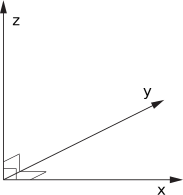
\includegraphics{fig-1-1}
 \caption{右手系座標軸}
 \label{fig:1.1}
\end{figure}



\section{テンソル}
\label{sec:1.2}
テンソル項は,特定の空間に属していて特定の数学的規則に従うような
実体について記述します.
簡潔にいえば,テンソルは単位基底ベクトルの組に対する
成分値の組で表現されます.
OpenFOAMではこの単位基底ベクトルは,
\index{ざひょうじく@座標軸!みぎてけいデカルトざひょうけい@右手系デカルト座標系}%
右手系デカルト座標軸$x$,$y$,$z$にそれぞれ沿った
$\mathbf{e}_{x}$,$\mathbf{e}_{y}$,$\mathbf{e}_{z}$になります.
したがって,これらの基底ベクトルは直交,すなわち互いに直角です.
すべてのテンソルは以下のような属性をもっています.
\begin{description}
 \item[次元] そのテンソルが属する特定の空間の次元$d$.
            OpenFOAMでは$d = 3$
 \item[ランク]
\index{テンソル!ランク}%
            成分値の数が$d^{r}$となるような整数$r \ge 0$
\end{description}
OpenFOAM~1.xが3
\index{テンソル!じげん@次元}%
次元であることから,
ランク$0$〜$3$のテンソルが標準で用意されていますが,
この基本のランクの設定は自由に拡張できるように書かれています.
ランク$0$と$1$のテンソルは,
\index{スカラ}%
スカラおよび
\index{ベクトル}%
ベクトルとしてのほうが
よく知られており読者にも身近でしょうが,
ランク$2$と$3$のテンソルにはあまりなじみがないかもしれません.
確認のために,OpenFOAM~1.xが標準で提供している
すべてのランクのテンソルを以下で復習しておきましょう.
\begin{description}
 \item[ランク0「スカラ」] 一つの実数で表せるあらゆる物理量で,
            イタリック体で表記されます.
            例えば,質量$m$,体積$V$,圧力$p$,そして粘性係数$\mu$です.
 \item[ランク1「ベクトル」] 大きさと方向で表現できる物理量です.
            成分表示では,ベクトル$\bm{a} = (a_{1},\ a_{2},\ a_{3})$は
            デカルト座標系の$x$軸,$y$軸,$z$軸成分をそれぞれ表します.
            同じベクトルを添字表記では$a_{i}$,$i = 1,\ 2,\ 3$と書けます.
            ただし,3次元を扱っていることは明らかなので
            本書では添字リスト$i = 1,\ 2,\ 3$は省略します.
 \item[ランク2「テンソル」] または
\index{テンソル!2かい@2階}%
「2階のテンソル」$\bm{T}$は
            以下のように行列で表現できる9\nobreak 個の要素をもっています.
            \begin{align}
             \label{eq:1.1}
             \bm{T} &= T_{ij}
             = \begin{pmatrix}
                T_{11} & T_{12} & T_{13} \\
                T_{21} & T_{22} & T_{23} \\
                T_{31} & T_{32} & T_{33}
               \end{pmatrix}
            \end{align}
            $r = 2$なので,要素$T_{ij}$は二つの添字で表されます.
            以下では添字のリスト$i,\ j = 1,\ 2,\ 3$は省略します.
            $i = j$の要素は対角要素とよばれ,
            $i \ne j$の要素は非対角要素とよばれます.
            対角要素を交差して要素を入れ替えることにより,
            以下のような$\bm{T}$の
\index{テンソル!てんち@転置}%
            \emph{転置}が得られます.
            \begin{align}
             \label{eq:1.2}
             \bm{T}^{\mathrm{T}} &= T_{ji}
             = \begin{pmatrix}
                T_{11} & T_{21} & T_{31} \\
                T_{12} & T_{22} & T_{32} \\
                T_{13} & T_{23} & T_{33}
               \end{pmatrix}
            \end{align}
            注意:ランク3以上のテンソルが出現することは非常にまれなので,
            多くの場合,ランク2のテンソルは単に「テンソル」とよばれます.
 \item[ランク2(対称)]
\index{テンソル!2かいたいしょう@2階対称}%
            「対称」というのは,対角方向に対称,
            つまり$T_{ij} = T_{ji}$であることを表します.
            この場合$T_{12} = T_{21}$,$T_{13} = T_{31}$,
            $T_{23} = T_{32}$なので,独立な要素は6個だけになります.
            対称テンソルであれば9個より6個の要素を保存するほうがメモリを節約できるので,
            OpenFOAMでは対称テンソルと非対称テンソルを区別して扱います.
            連続体力学において遭遇するほとんどのテンソルは対称です.
 \item[ランク3]
\index{テンソル!3かい@3階}%
            27個の要素をもち,添字表記では$P_{ijk}$と書けますが,
            \autoref{eq:1.1}\hskip\xkanjiskip のように行列表示しようとすると非常に長くなります.
\item[ランク3(対称)]
\index{テンソル!3かいたいしょう@3階対称}%
           ランク3の対称テンソルは,OpenFOAMでは
           $P_{ijk} = P_{ikj} = P_{jik} = P_{jki} = P_{kij} = P_{kji}$として定義されており,
           したがって10個の独立した要素をもちます.
           さらに厳密にいえば,これは相等しい三つのベクトルの外積によってつくられます.
           外積については\autoref{ssec:1.3.4}で述べられています.
\end{description}


\subsection{テンソル表記}
\label{ssec:1.2.1}
本書は,空間3次元と時間からなる複雑な偏微分方程式の問題を扱う,数値連続体力学に関するものです.
まず最初に,簡潔でありながら明確な,方程式の表記方法を導入しておくことが不可欠です.
方程式を追いやすいようにするには,スカラ要素のリストを書くよりも,
それ自体にテンソルの概念が含められた一つのもので表記することが必要です.
加えて,あらゆるテンソル演算が,要素それぞれに体する演算ではなく
テンソル自体に対する演算である,とわかるような表記法であるべきです.

そういうわけで,この文書ではランク1以上のテンソル,
すなわちスカラ以外のすべてのテンソルについては
\index{テンソル!ひょうき@表記}%
\emph{テンソル表記}を採用し,
太字で,例えば$\bm{a}$のように表記します.
これは一つのシンボルで表され,非常にコンパクトであることから,
それ自体で一つの存在としてテンソルを把握しやすくなります.
欠点をあげるとすれば,太字のシンボルはランク0でないことは明らかですが,
そのランクがすぐには読み取れないことです.
しかしながら,シンボルを見れば何の物理量を表しているかがわかり,
直観的にランクもわかるので,実際にはそれほど問題になりません.
例えば,私たちは速度$\bm{U}$がランク1のテンソルであることを知っています.

さらにいえば,表記方法の選択を評価するもっと根本的な点は,
テンソルの数学的表現が座標系によって変化しないこと,
つまりベクトル$\bm{a}$がどこから観測するかに拘らず
同じベクトルであることです.
テンソル表記は,座標系に関する情報をいっさい含まないので,
このコンセプトに合っています.
しかし,他の表記,たとえば$a_{i}$のようにテンソルの成分個別の表示は
必然的に座標系の選択を意味してしまいます.
この望ましくない結果は,
一意でない,つまり座標系に依存する
値の組み合わせでテンソルが表現されることによります.

とはいえ本書では,主にテンソル演算を成分要素に展開するために,
\autoref{sec:1.2}で述べたような添字表記もときどき用います.
添字表記を用いる際には,和の規約を採用します.
これは,一つの項に同じ添字が2回現れたら,
その添字については該当する全ての数字,たとえば$1$,$2$,$3$をとり,
それらの和をとるというものです.
たとえば次のようになります.
\begin{align}
 \label{eq:1.3}
 a_{i}b_{i} = \sum^{3}_{i=1}a_{i}b_{i} = a_{1}b_{1} + a_{2}b_{2} + a_{3}b_{3}
\end{align}

添字が繰り返されたら和を意味するので,この文書では今後,記号$\sum$は省略します.



\section{テンソルの代数演算}
\label{sec:1.3}
この節では,OpenFOAMで利用できるテンソルの
\index{テンソル!だいすうえんざん@代数演算}%
代数演算をすべて紹介します.
まず,もっとも基本的なテンソル演算をおさらいしておきましょう.
\index{テンソル!かさん@加算}%
加算,
\index{テンソル!げんさん@減算}%
減算,そして
\index{テンソル!スカラのじょうさん@スカラの乗算}%
スカラの乗算と除算です.
加算と減算は,可換則と結合則の両方を満たし,
互いにランクの等しいテンソルどうしに限って意味をもちます.
これはテンソルの要素それぞれについて加算・減算を行う操作であり,
たとえば,二つのベクトル$\bm{a}$と$\bm{b}$の差は
\begin{align}
 \label{eq:1.4}
 \bm{a} - \bm{b} = a_{i} - b_{i} = (a_{1} - b_{1},\ a_{2} - b_{2},\ a_{3} - b_{3})
\end{align}
となります.
テンソル$\bm{a}$にスカラ$s$をかける乗算も同様に可換則と結合則を満たし,
テンソルの要素すべてにスカラを乗じる操作です.
たとえば,次のようになります.
\begin{align}
 \label{eq:1.5}
 s\bm{a} = sa_{i} = (sa_{1},\ sa_{2},\ sa_{3})
\end{align}
テンソル$\bm{a}$と
\index{テンソル!スカラのじょさん@スカラの除算}%
スカラの除算は,
スカラが演算の第2引数となっているときにのみ意味をもちます.
つまり,次のとおりです.
\begin{align}
 \label{eq:1.6}
 \frac{\bm{a}}{s} = \frac{a_{i}}{s}
 = \left(\frac{a_{1}}{s},\ \frac{a_{2}}{s},\ \frac{a_{3}}{s}\right)
\end{align}
これ以降の節で述べる上記以外の演算は,
ランク1以上のテンソルどうしの,
さらに複雑な積の組み合わせとなっています.


\subsection{内積}
\label{ssec:1.3.1}
\index{テンソル!ないせき@内積}%
内積は,ランク$r_{1}$と$r_{2}$の任意の二つのテンソルを
ランク$r = r_{1} + r_{2} - 2$のテンソルにする演算です.
ランク3までのテンソルの内積演算を以下に示します.
\begin{itemize}
 \item 二つのベクトル$\bm{a}$と$\bm{b}$の内積は可換であり,
       以下のスカラ$s = \bm{a} \inProd \bm{b}$をつくります.
       \begin{align}
        \label{eq:1.7}
        s = a_{i}b_{i} = a_{1}b_{2} + a_{2}b_{2} + a_{3}b_{3}
       \end{align}
 \item テンソル$\bm{T}$とベクトル$\bm{a}$の内積は
       ベクトル$\bm{b} = \bm{T} \inProd \bm{a}$をつくります.
       これは,見やすいように列ベクトルで書くと,以下のようになります.
       \begin{align}
        \label{eq:1.8}
        b_{i} = T_{ij}a_{j} =
        \begin{pmatrix}
         T_{11}a_{1} + T_{12}a_{2} + T_{13}a_{3} \\
         T_{21}a_{1} + T_{22}a_{2} + T_{23}a_{3} \\
         T_{31}a_{1} + T_{32}a_{2} + T_{33}a_{3}
        \end{pmatrix}
       \end{align}
       もし$\bm{T}$が対称でなければ,
       $\bm{b} = \bm{a} \inProd \bm{T} = \bm{T}^{\mathrm{T}} \inProd \bm{a}$は
       以下のようになり,この演算は可換ではありません.
       \begin{align}
        \label{eq:1.9}
        b_{i} = a_{j}T_{ji} =
        \begin{pmatrix}
         a_{1}T_{11} + a_{2}T_{21} + a_{3}T_{31} \\
         a_{1}T_{12} + a_{2}T_{22} + a_{3}T_{32} \\
         a_{1}T_{13} + a_{2}T_{23} + a_{3}T_{33}
        \end{pmatrix}
       \end{align}
 \item 二つのテンソル$\bm{T}$と$\bm{S}$の内積は,
       以下のような成分をもつテンソル$\bm{P} = \bm{T} \inProd \bm{S}$をつくります.
       \begin{align}
        \label{eq:1.10}
        P_{ij} = T_{ik}S_{kj}
       \end{align}
       これは$\bm{T} \inProd \bm{S} =
       (\bm{S}^{\mathrm{T}} \inProd \bm{T}^{\mathrm{T}})^{\mathrm{T}}$となり,非可換です.
 \item ベクトル$\bm{a}$と3階のテンソル$\bm{P}$の内積は,
       以下のような成分をもつ2階のテンソル$\bm{T} = \bm{a} \inProd \bm{P}$をつくります.
       \begin{align}
        \label{eq:1.11}
        T_{ij} = a_{k}P_{kij}
       \end{align}
       やはりこれも非可換で,
       $\bm{T} = \bm{P} \inProd \bm{a}$は次のようになります.
       \begin{align}
        \label{eq:1.12}
        T_{ij} = P_{ijk}a_{k}
       \end{align}
 \item 2階のテンソル$\bm{T}$と3階のテンソル$\bm{P}$の内積は,
       以下のような成分をもつ3階のテンソル$\bm{Q} = \bm{T} \inProd \bm{P}$をつくります.
       \begin{align}
        \label{eq:1.13}
        Q_{ijk} = T_{il}P_{ljk}
       \end{align}
       やはりこれも非可換で,
       $\bm{Q} = \bm{P} \inProd \bm{T}$は次のようになります.
       \begin{align}
        \label{eq:1.14}
        Q_{ijk} = P_{ijl}T_{lk}
       \end{align}
\end{itemize}


\subsection{二つのテンソルの二重内積}
\label{ssec:1.3.2}
二つの2階テンソル$\bm{T}$と$\bm{S}$の
\index{テンソル!にじゅうないせき@二重内積}%
二重内積は,
スカラ$s = \bm{T} \biInProd \bm{S}$をつくります.
これは,テンソル成分の9個の積の和として得られます.
\begin{align}
 \label{eq:1.15}
 \begin{aligned}
  s = T_{ij}S_{ij} &= T_{11}S_{11} + T_{12}S_{12} + T_{13}S_{13} + {} \\
  &\hphantom{{}={}} T_{21}S_{21} + T_{22}S_{22} + T_{23}S_{23} + {} \\
  &\hphantom{{}={}} T_{31}S_{31} + T_{32}S_{32} + T_{33}S_{33}
 \end{aligned}
\end{align}

2階のテンソル$\bm{T}$と3階のテンソル$\bm{P}$の二重内積は,
次のような成分をもつベクトル$\bm{a} = \bm{T} \biInProd \bm{P}$をつくります.
\begin{align}
 \label{eq:1.16}
 a_{i} = T_{jk}P_{jki}
\end{align}
これは非可換で,$\bm{a} = \bm{P} \biInProd \bm{T}$は次のようになります.
\begin{align}
 \label{eq:1.17}
 a_{i} = P_{ijk}T_{jk}
\end{align}


\subsection{二つの3階テンソルの三重内積}
\label{ssec:1.3.3}
二つの3階テンソル$\bm{P}$と$\bm{Q}$の
\index{テンソル!さんじゅうないせき@三重内積}%
三重内積は,
スカラ$s = \bm{P} \triInProd \bm{Q}$をつくります.
これは,テンソル成分の27個の積の和として得られます.
\begin{align}
 \label{eq:1.18}
 \begin{aligned}
  s = P_{ijk}Q_{ijk}
 \end{aligned}
\end{align}


\subsection{外積}
\label{ssec:1.3.4}
\index{テンソル!がいせき@外積}%
外積は,以下のようなベクトルやテンソルどうしの演算です.
\begin{itemize}
 \item 二つのベクトル$\bm{a}$と$\bm{b}$の外積は非可換で,
       以下のような成分をもつテンソル
       $\bm{T} = \bm{a}\bm{b} = (\bm{b}\bm{a})^{\mathrm{T}}$をつくります.
       \begin{align}
        \label{eq:1.19}
        T_{ij} = a_{i}b_{j} =
        \begin{pmatrix}
         a_{1}b_{1} & a_{1}b_{2} & a_{1}b_{3} \\
         a_{2}b_{1} & a_{2}b_{2} & a_{2}b_{3} \\
         a_{3}b_{1} & a_{3}b_{2} & a_{3}b_{3}
        \end{pmatrix}
       \end{align}
 \item ベクトル$\bm{a}$と2階のテンソル$\bm{T}$との外積は,
       以下のような成分をもつ3階のテンソル
       $\bm{P} = \bm{a}\bm{T}$をつくります.
       \begin{align}
        \label{eq:1.20}
        P_{ijk} = a_{i}T_{jk}
       \end{align}
       これは非可換で,
       $\bm{P} = \bm{T}\bm{a}$は以下のようになります.
       \begin{align}
        \label{eq:1.21}
        P_{ijk} = T_{ij}a_{k}
       \end{align}
\end{itemize}


\subsection{二つのベクトルのクロス積}
\label{ssec:1.3.5}
\index{テンソル!ベクトルのクロスせき@ベクトルのクロス積}%
クロス積はベクトルだけに存在する演算です.
二つのベクトル$\bm{a}$と$\bm{b}$について,
これらのクロス積は以下のような成分をもつベクトル
$\bm{c} = \bm{a} \times \bm{b}$をつくります.
\begin{align}
 \label{eq:1.22}
 c_{i} = e_{ijk}a_{j}b_{k}
 = (a_{2}b_{3} - a_{3}b_{2},\ a_{3}b_{1} - a_{1}b_{3},\  a_{1}b_{2} - a_{2}b_{1})
\end{align}
ここで
\index{ちかんきごう@置換記号}%
\OFemph{置換記号}は以下のように定義されます.
\begin{align}
 \label{eq:1.23}
 e_{ijk} =
 \begin{cases}
  0 & \text{いずれか二つの添字が等しいとき} \\
  +1 & \text{$i,\ j,\ k$が$1,\ 2,\ 3$の偶置換のとき} \\
  -1 & \text{$i,\ j,\ k$が$1,\ 2,\ 3$の奇置換のとき}
 \end{cases}
\end{align}
偶置換とは$123$,$231$および$312$であり,
奇置換は$132$,$213$および$321$です.


\subsection{その他の一般的なテンソル演算}
\label{ssec:1.3.6}
OpenFOAMで使われる,やや一般的でない演算や専門用語を以下に示します.
\begin{description}
 \item[二乗]
\index{テンソル!にじょう@二乗}%
            テンソルの二乗は,それ自身とのテンソル外積で定義されます.
            例えば,ベクトル$\bm{a}$の二乗は$\bm{a}^{2} = \bm{a}\bm{a}$です.
 \item[$n$乗]
\index{テンソル!nじょう@$n$乗}%
            テンソルの$n$乗は,それ自身との$n$回のテンソル外積で定義されます.
            例えば,ベクトル$\bm{a}$の$3$乗は$\bm{a}^{3} = \bm{a}\bm{a}\bm{a}$です.
 \item[平方絶対値]
\index{テンソル!へいほうぜったいち@平方絶対値}%
            テンソルの平方絶対値は,それ自身との$r$テンソルの$r$重内積で,スカラとなります.
            例えば,2階テンソル$\bm{T}$については,$|\bm{T}|^{2} = \bm{T} \biInProd \bm{T}$です.
 \item[絶対値]
\index{テンソル!ぜったいち@絶対値}%
            平方絶対値の平方根です.
            例えば,テンソル$\bm{T}$については,$|\bm{T}| = \sqrt{\bm{T} \biInProd \bm{T}}$です.
            単位長さのベクトルは
\index{ベクトル!たんい@単位}%
            \OFemph{単位ベクトル}とよばれます.
 \item[最大成分]
\index{テンソル!さいだいせいぶん@最大成分}%
            符号も考慮した最大の値をもつテンソルの成分です.つまり最大の絶対値ではありません.
 \item[最小成分]
\index{テンソル!さいしょうせいぶん@最小成分}%
            最小の値をもつテンソルの成分です.
 \item[成分平均値]
\index{テンソル!せいぶんへいきんち@成分平均値}%
            テンソルのすべての成分の平均値です.
 \item[スケール] 名前のとおり,
\index{テンソル!スケールかんすう@スケール関数}%
            スケール関数は,
            あるテンソルの成分を同じランクの他のテンソルの成分でスケーリングします.
            これは二つのテンソルの対応する成分同士の積で評価されます.
            例えば,ベクトル$\bm{a}$のベクトル$\bm{b}$によるスケーリングは,
            以下のような成分のベクトル$\bm{c}$をつくります.
            \begin{align}
             \label{eq:1.24}
             c_{i} = \mathop{\mathrm{scale}}(\bm{a},\ \bm{b})
             = (a_{1}b_{1},\ a_{2}b_{2},\ a_{3}b_{3})
            \end{align}
\end{description}


\subsection{幾何変換と単位テンソル}
\label{ssec:1.3.7}
2階のテンソル$\bm{T}$は線形ベクトル関数,
すなわち,内積$\bm{b} = \bm{T} \inProd \bm{a}$によって,
あるベクトル$\bm{a}$を別のベクトル$\bm{b}$に結びつける関数として,
厳密に定義されます.
$x,\ y,\ z$座標系から新しい座標系$x^{*},\ y^{*},\ z^{*}$への
あるテンソルの座標
\index{テンソル!きかへんかん@幾何変換}%
\index{テンソル!へんかん@変換}%
変換として機能するように,
$\bm{T}$の成分を選ぶことができます.
このとき$\bm{T}$を\OFemph{変換テンソル}とよびます.
スカラは変換によって変化しませんが,
ベクトル$\bm{a}$は
\begin{align}
 \label{eq:1.25}
 \bm{a}^{*} = \bm{T} \inProd \bm{a}
\end{align}
のように$\bm{a}^{*}$に変換されます.
2階のテンソル$\bm{S}$は
\begin{align}
 \label{eq:1.26}
 \bm{S}^{*} = \bm{T} \inProd \bm{S} \inProd \bm{T}^{\mathrm{T}}
\end{align}
に従って$\bm{T}^{*}$に変換されます.

\index{テンソル!たんい@単位}%
\OFemph{単位テンソル}$\bm{I}$は,
あるテンソルをそれ自身に変換するという条件から定義されます.
すべてのベクトル$\bm{a}$に対して
\begin{align}
 \label{eq:1.27}
 \bm{a} = \bm{I} \inProd \bm{a}
\end{align}
となり,つまり
\begin{align}
 \label{eq:1.28}
 \bm{I} = \delta_{ij} =
 \begin{pmatrix}
  1 & 0 & 0 \\
  0 & 1 & 0 \\
  0 & 0 & 1 \\
 \end{pmatrix}
\end{align}
となります.ここで,$\delta_{ij}$は
\index{クロネッカーのデルタ}%
\OFemph{クロネッカーのデルタ}として知られています.


\subsection{便利なテンソルの恒等式}
\label{ssec:1.3.8}
さまざまな
\index{テンソル!こうとうしき@恒等式}%
恒等式を以下に示します.
これらは,関連するすべての微分が存在して連続であるという仮定のもとで証明できます.
スカラ$s$とベクトル$\bm{a}$および$\bm{b}$を用いて表記しています.
%%% 訳注:原文では$\bm{b}$への言及が抜けている.
\begin{align}
 \label{eq:1.29}
 \begin{aligned}
  \nabla \inProd (\nabla \times \bm{a}) &\equiv 0 \\
  \nabla \times (\nabla s) &\equiv \bm{0} \\
  \nabla \inProd (s\bm{a}) &\equiv s\nabla \inProd \bm{a} + \bm{a} \inProd \nabla s \\
  \nabla \times (s\bm{a}) &\equiv s\nabla \times \bm{a} + \nabla s \times \bm{a} \\
  \nabla (\bm{a} \inProd \bm{b})
    &\equiv \bm{a} \times (\nabla \times \bm{b}) + \bm{b} \times (\nabla \times \bm{a})
            + (\bm{a} \inProd \nabla)\bm{b} + (\bm{b} \inProd \nabla)\bm{a} \\
  \nabla \inProd (\bm{a} \times \bm{b})
    &\equiv \bm{b} \inProd (\nabla \times \bm{a}) - \bm{a} \inProd (\nabla \times \bm{b}) \\
  \nabla \times (\bm{a} \times \bm{b})
    &\equiv \bm{a}(\nabla \inProd \bm{b}) - \bm{b}(\nabla \inProd \bm{a})
            + (\bm{b} \inProd \nabla)\bm{a} - (\bm{a} \inProd \nabla)\bm{b} \\
  \nabla \times (\nabla \times \bm{a})
    &\equiv \nabla (\nabla \inProd \bm{a}) - \Laplacian\bm{a} \\
  (\nabla \times \bm{a})
    &\equiv \bm{a} \inProd (\nabla \bm{a}) - \nabla (\bm{a} \inProd \bm{a})
 \end{aligned}
\end{align}
添字表記の数式を操作するときには,
以下の$e$--$\delta$恒等式を知っていると役立つことがあります.
\begin{align}
 \label{eq:1.30}
 e_{ijk}e_{irs} = \delta_{jr}\delta_{ks} - \delta_{js}\delta_{kr}
\end{align}


\subsection{2階テンソル特有の演算}
\label{ssec:1.3.9}
以下に示すように,2階テンソルの成分を操作する様々な演算があります.
\begin{description}
 \item[転置]
\index{テンソル!てんち@転置}%
            \autoref{eq:1.2}で示したように,
            テンソル$\bm{T} = T_{ij}$の転置は$\bm{T}^{\mathrm{T}} = T_{ji}$です.
 \item[対称テンソルと歪(反対称)テンソル] \autoref{sec:1.2}で述べたように,
            $\bm{T} = \bm{T}^{\mathrm{T}}$のように
            成分が対角方向に対称なテンソルを
\index{テンソル!たいしょうテンソル@対称テンソル}%
            対称テンソルとよびます.
\index{テンソル!わいテンソル@歪テンソル}%
            歪テンソルもしくは
\index{テンソル!はんたいしょうテンソル@反対称テンソル|see{歪テンソル}}%
            反対称テンソルは$\bm{T} = -\bm{T}^{\mathrm{T}}$であり,
            当然$T_{11} = T_{22} = T_{33} = 0$となります.
            あらゆる2階テンソルは,以下のように対称テンソルと歪テンソルに分割できます.
            \begin{align}
             \label{eq:1.31}
             \bm{T} = \underbrace{\frac{1}{2}(\bm{T} + \bm{T}^{\mathrm{T}})}_{\text{対称テンソル}}
             + \underbrace{\frac{1}{2}(\bm{T} - \bm{T}^{\mathrm{T}})}_{\text{歪テンソル}}
             = \mathop{\mathrm{symm}}\bm{T} + \mathop{\mathrm{skew}}\bm{T}
            \end{align}
 \item[トレース] テンソル$\bm{T}$の
\index{テンソル!トレース}%
            トレースは対角成分の総和をとったスカラです.
            \begin{align}
             \label{eq:1.32}
             \mathop{\mathrm{tr}}\bm{T} = T_{11} + T_{22} + T_{33}
            \end{align}
 \item[対角] 2階テンソル$\bm{T}$の
\index{テンソル!たいかく@対角}%
            対角成分を成分とするベクトルを返します.
            \begin{align}
             \label{eq:1.33}
             \mathop{\mathrm{diag}}\bm{T} = (T_{11},\ T_{22},\ T_{33})
            \end{align}
 \item[偏差テンソルと静水圧テンソル] あらゆる2階テンソル$\bm{T}$は,
            $\mathop{\mathrm{tr}}T = 0$となる偏差成分と,
            スカラ$s$に対して$\bm{T} = s\bm{I}$となる静水圧成分に分割できます.
            あらゆる2階テンソルは,以下のように
\index{テンソル!へんさテンソル@偏差テンソル}%
            偏差テンソルと
\index{テンソル!せいすいあつテンソル@静水圧テンソル}%
            静水圧テンソルに分割できます.
            \begin{align}
             \label{eq:1.34}
             \bm{T} = \underbrace{\bm{T}
             - \frac{1}{3}(\mathop{\mathrm{tr}}\bm{T})\bm{I}}_{\text{偏差テンソル}}
             + \underbrace{\frac{1}{3}(\mathop{\mathrm{tr}}\bm{T})\bm{I}}_{\text{静水圧テンソル}}
             = \mathop{\mathrm{dev}}\bm{T} + \mathop{\mathrm{hyd}}\bm{T}
            \end{align}
 \item[行列式] 2階テンソルの
\index{テンソル!ぎょうれつしき@行列式}%
            行列式は以下で与えられます.
            \begin{align}
             \label{eq:1.35}
             \begin{split}
              \det\bm{T} &= \begin{vmatrix}
                             T_{11} & T_{12} & T_{13} \\
                             T_{21} & T_{22} & T_{23} \\
                             T_{31} & T_{32} & T_{33}
                            \end{vmatrix} \\
              &= T_{11}(T_{22}T_{33} - T_{23}T_{32})
              - T_{12}(T_{21}T_{33} - T_{23}T_{31})
              + T_{13}(T_{21}T_{32} - T_{22}T_{31}) \\
              &= \frac{1}{6}e_{ijk}e_{pqr}T_{ip}T_{jq}T_{kr}
             \end{split}
            \end{align}
 \item[余因子] テンソルのある成分が属する行と列を取り除いてできた部分を
            $2 \times 2$の行列式として評価したものを,
            テンソルのそれぞれの成分に対する小行列式といいます.
            例えば,$T_{12}$に対する小行列式は
            \begin{align}
             \label{eq:1.36}
             \begin{vmatrix}
              \rlap{\rule[4pt]{67pt}{.4pt}}T_{11} &
              \rlap{\hskip5pt\smash{\rule[-36pt]{.4pt}{44pt}}}T_{12} & T_{13} \\
              T_{21} & T_{22} & T_{23} \\
              T_{31} & T_{32} & T_{33}
             \end{vmatrix}
             = \begin{vmatrix}
                T_{21} & T_{23} \\
                T_{31} & T_{33}
               \end{vmatrix}
             = T_{21}T_{33} - T_{23}T_{31}
            \end{align}
            となります.
\index{テンソル!よいんし@余因子}%
            余因子とは,それぞれの成分の位置に応じて以下のルールで符号付けした小行列式です.
            \begin{align}
             \label{eq:1.37}
             \begin{aligned}
              &\text{$i + j$が偶数ならば$+$} \\
              &\text{$i + j$が奇数ならば$-$}
             \end{aligned}
            \end{align}
            $\bm{T}$の余因子は以下のようになります.
            \begin{align}
             \label{eq:1.38}
             \mathop{\mathrm{cof}}\bm{T} = \frac{1}{2}e_{jkr}e_{ist}T_{sk}T_{tr}
            \end{align}
 \item[逆元]
\index{テンソル!ぎゃくげん@逆元}%
            テンソルの逆元は以下で評価されます.
            \begin{align}
             \label{eq:1.39}
             \mathop{\mathrm{inv}}\bm{T}
             = \frac{\mathop{\mathrm{cof}}\bm{T}^{\mathrm{T}}}{\det\bm{T}}
            \end{align}
 \item[ホッジ双対]
\index{テンソル!ホッジそうつい@ホッジ双対}%
            テンソルのホッジ双対とは,以下のような成分をもつベクトルです.
            \begin{align}
             \label{eq:1.40}
             \mathop{*}\bm{T} = (T_{23},\ -T_{13},\ T_{12})
            \end{align}
\end{description}


\subsection{スカラ特有の演算}
\label{ssec:1.3.10}
OpenFOAMは,スカラを扱うよく知られた関数のほとんどをサポートしています.
例えば平方根,指数,対数,正弦,余弦などで,
これらのリストが\autoref{tbl:1.2}にあります.
OpenFOAMでは,これらに加えて以下の$3$種類の関数も定義されています.
\begin{description}
 \item[符号] スカラ$s$の符号は以下のように得られます.
            \begin{align}
             \label{eq:1.41}
             \mathop{\mathrm{sgn}}(s) =
             \begin{cases}
              1 & \text{$s \ge 0$のとき} \\
              -1 & \text{$s < 0$のとき}
             \end{cases}
            \end{align}
 \item[正数] スカラ$s$に対して以下のように得られます.
            \begin{align}
             \label{eq:1.42}
             \mathop{\mathrm{pos}}(s) =
             \begin{cases}
              1 & \text{$s \ge 0$のとき} \\
              0 & \text{$s < 0$のとき}
             \end{cases}
            \end{align}
 \item[制限] スカラ$s$のスカラ$n$による制限は以下のようになります.
            \begin{align}
             \label{eq:1.43}
             \mathop{\mathrm{limit}}(s,\ n) =
             \begin{cases}
              s & \text{$s < n$のとき} \\
              0 & \text{$s \ge n$のとき}
             \end{cases}
            \end{align}
\end{description}



\section{OpenFOAMのテンソルクラス}
\label{sec:1.4}
OpenFOAMには,これまでに述べたようなテンソル数学のためのクラス群を含んだ
\index{primitive@\OFclass{primitive}!ライブラリ}%
\index{ライブラリ!primitive@\OFclass{primitive}}%
\OFclass{primitive}というC++のクラスライブラリがあります.
OpenFOAMで標準的に使える基本テンソル
\index{テンソル!OpenFOAMにおけるクラス}%
クラスを\autoref{tbl:1.1}に列挙します.
この表にはテンソルの個別の成分にアクセスするための関数,
いわゆる
\index{アクセスかんすう@アクセス関数}%
アクセス関数も列挙してあります.


\begin{table}[ht]
 %#! uplatex ProgrammersGuideJa
\begin{tabular}{clll}
 ランク & 名称 & 基本クラス & アクセス関数 \\
 \hline
 \tblstrut
 $0$ & スカラ &
\index{クラス!scalar@\OFclass{scalar}}%
\index{scalarクラス@\OFclass{scalar}クラス}%
         \OFclass{scalar} & \\
 $1$ & ベクトル &
\index{クラス!vector@\OFclass{vector}}%
\index{vectorクラス@\OFclass{vector}クラス}%
         \OFclass{vector} & \OFkeyword{x()}, \OFkeyword{y()}, \OFkeyword{z()} \\
 $2$ & テンソル &
\index{クラス!tensor@\OFclass{tensor}}%
\index{tensorクラス@\OFclass{tensor}クラス}%
         \OFclass{tensor} & \OFkeyword{xx()}, \OFkeyword{xy()}, \OFkeyword{xz()}, ... \\
 \hline
\end{tabular}

 \caption{OpenFOAMにおける基本テンソルクラス}
 \label{tbl:1.1}
\end{table}


テンソル
\begin{align}
 \label{eq:1.44}
 \bm{T} =
 \begin{pmatrix}
  1 & 2 & 3 \\
  4 & 5 & 6 \\
  7 & 8 & 9
 \end{pmatrix}
\end{align}
は,OpenFOAMでは次の1行で宣言できます.
\begin{OFverbatim}[terminal]
tensor T(1, 2, 3, 4, 5, 6, 7, 8, 9);
\end{OFverbatim}

アクセス関数\OFkeyword{xz()}で
成分$T_{13}$つまり$T_{xz}$にアクセスできます.
例えば,コード
\begin{OFverbatim}[terminal]
Info << ``Txz = '' << T.xz() << endl;
\end{OFverbatim}
は,以下を画面に出力します.
\begin{OFverbatim}[terminal]
Txz = 3
\end{OFverbatim}


\subsection{OpenFOAMにおけるテンソルの代数演算}
\label{ssec:1.4.1}
\autoref{sec:1.3}で述べたすべての
\index{テンソル!OpenFOAMにおけるテンソルのだいすうえんざん@OpenFOAMにおけるテンソルの代数演算}%
代数演算は,
OpenFOAMのテンソルクラスに対して,
数学の表記法によく似た構文で利用できます.
いくつかの関数は,例えば\OFkeyword{symm()}のように,単に記述的な関数で表現しますが,
その他については,例えば\hskip\xkanjiskip\OFkeyword{*}\hskip\xkanjiskip のような演算子記号でも使用できます.
すべての関数を\autoref{tbl:1.2}に列挙します.


\vskip\floatsep
\begingroup
 \small
% \begin{table}[ht]
 \LTXtable{.8\textwidth}{tbl/tbl-1-2}
% 原文では,逆三角関数がプログラミング言語のように
% asin,acos,atan などとされているが,
% あまり数学で使われる表記ではないと思われるため,
% ここでは arcsin,arccos,arctan などとした.
 \addtocounter{table}{-1}%
 \tblcaption{OpenFOAMにおけるテンソルの代数演算}
 \label{tbl:1.2}
% \end{table}
\endgroup
\vskip\floatsep



\section{物理次元の単位}
\label{sec:1.5}
連続体力学では,物理量はある選ばれた単位で記述されます.
例えば,質量はキログラム ($\unit*{kg}$),
体積は立方メートル ($\unit*{m^{3}}$),
圧力はパスカル ($\unit*{kg\,m^{-1}\,s^{-2}}$).
これらの物理量に対する代数演算は,
\index{たんい@単位!けいりょう@計量}%
計量単位を一致させて行わなければなりません.
特に,加算,減算,等価判定は,同じ単位の物理量に対してのみ,物理的な意味をもちます.
無意味な演算の実装を予防するために,
\index{じげん@次元!OpenFOAMにおけるじげんチェック@OpenFOAMにおける次元チェック}%
OpenFOAMはユーザがあらゆるテンソルに物理次元の単位を付加することを推奨し,
これによりあらゆるテンソル演算の際に次元のチェックが行われます.

単位は,例えば以下のように,\OFclass{dimensionSet}クラスで定義されます.
\begin{OFverbatim}[terminal]
dimensionSet pressureDims(1, -1, -2, 0, 0, 0, 0);
\end{OFverbatim}


\begin{table}[ht]
 %#! platex ProgrammersGuideJa
\begin{tabular}{clll}
 No. & 物理量 & 単位 & 記号 \\
 \hline
 \tblstrut
 1 & 質量 & キログラム & $\mathrm{kg}$ \\
 2 & 長さ & メートル & $\mathrm{m}$ \\
 3 & 時間 & 秒 & $\mathrm{s}$ \\
 4 & 熱力学温度 & ケルビン & $\mathrm{K}$ \\
 5 & 物質量 & モル & $\mathrm{mol}$ \\
 6 & 電流 & アンペア & $\mathrm{A}$ \\
 7 & 光度 & カンデラ & $\mathrm{cd}$ \\
 \hline
\end{tabular}

 \caption{SI基本計量単位}
 \label{tbl:1.3}
\end{table}


ここで,それぞれの値は,\autoref{tbl:1.3}に列挙した
SI基本計量単位それぞれの指数を示しています.
このコードでは\OFkeyword{pressureDims}を,
圧力$\unit*{kg\,m^{-1}\,s^{-2}}$の\OFclass{dimensionSet}として宣言しています.
すなわち\OFkeyword{pressureDims}の引数配列の最初の項目$1$は$\unit*{kg^{1}}$を表し,
二つめの$-1$は$\unit*{m^{-1}}$を表す,などのようにです.
単位付きのテンソルは
\index{dimensioned<Type>@\OFclass{dimensioned<Type>}!テンプレートクラス}%
\OFclass{dimensioned<Type>}テンプレートクラスで定義されます.
\OFclass{<Type>}は\OFclass{scalar},\OFclass{vector},\OFclass{tensor}などです.
この
\index{テンプレートクラス!dimensioned<Type>@\OFclass{dimensioned<Type>}}%
\OFclass{dimensioned<Type>}は,
\index{word@\OFclass{word}!クラス}%
\index{クラス!word@\OFclass{word}}%
\OFclass{word}クラスの変数名,
\OFclass{<Type>}の値,そして
\index{クラス!dimensionSet@\OFclass{dimensionSet}}%
\index{dimensionSet@\OFclass{dimensionSet}!クラス}%
\OFclass{dimensionSet}を保持します.

\begin{OFverbatim}[terminal]
dimensionedTensor sigma
    (
        "sigma",
        dimensionSet(1, -1, -2, 0, 0, 0, 0),
        tensor(1e6, 0, 0, 0, 1e6, 0, 0, 0, 1e6),
    );
\end{OFverbatim}
は,圧力あるいは応力としてしかるべき次元をもつ以下のテンソルをつくります.
\begin{align}
 \label{eq:1.45}
 \sigma =
 \begin{pmatrix}
  10^{6} & 0 & 0 \\
  0 & 10^{6} & 0 \\
  0 & 0 & 10^{6} \\
 \end{pmatrix}
\end{align}


%#! platex ProgrammersGuideJa
\chapter{離散化手法}
\label{chap:2}
これまではテンソル代数について議論してきました.
我々が解きたい偏微分方程式は,テンソルの時間および空間に対する微分に関するものです.
したがって,\OFemph{テンソル場},すなわち時間および空間の領域にわたって変化するテンソルへと,
表現を拡張する必要があります.
この章では,まずはじめに登場するすべての微分演算の数学的表現を解説します.
そして,OpenFOAMではテンソル場がどのように構築されているのか,
これらの場の微分はどのようにして代数式へと離散化されるのかを紹介します.



\section{微分演算子}
\label{sec:2.1}
空間微分を定義する前に,ベクトル演算子ナブラ$\nabla$を紹介します.
添字表記では$\partial_{i}$と書かれます.
\begin{align}
 \label{eq:2.1}
 \nabla \equiv \partial_{i} \equiv \frac{\partial}{\partial x_{i}}
 \equiv \left(\frac{\partial}{\partial x_{1}},\
 \frac{\partial}{\partial x_{2}},\
 \frac{\partial}{\partial x_{3}}\right)
\end{align}
ナブラ演算子は,以下のルールに従う便利な表記法です.
\begin{itemize}
 \item テンソルに作用するときは,自身の右側に向かって,通常の積の微分のルールに従う.
       例えば$\partial_{i}ab = (\partial_{i}a)b + a(\partial_{i}b)$
 \item それ以外の場合,ナブラ演算子は代数演算における通常のベクトルと同様に振る舞う.
\end{itemize}


\subsection{勾配}
\label{ssec:2.1.1}
スカラ場$s$が定義されていて,連続微分可能ならば,
$s$の勾配$\nabla s$は以下のベクトル場となります.
\begin{align}
 \label{eq:2.2}
 \nabla s = \partial_{i}s
 = \left(\frac{\partial s}{\partial x_{1}},\
 \frac{\partial s}{\partial x_{2}},\
 \frac{\partial s}{\partial x_{3}}\right)
\end{align}

勾配はあらゆるテンソル場に作用し,一つランクの高いテンソル場を作ります.
例えば,ベクトル場$\bm{a}$の勾配は,以下の2階テンソルです.
\begin{align}
 \label{eq:2.3}
 \nabla\bm{a} = \partial_{i}a_{j} =
 \begin{pmatrix}
  \partial a_{1}/\partial x_{1} & \partial a_{2}/\partial x_{1} & \partial a_{3}/\partial x_{1} \\
  \partial a_{1}/\partial x_{2} & \partial a_{2}/\partial x_{2} & \partial a_{3}/\partial x_{2} \\
  \partial a_{1}/\partial x_{3} & \partial a_{2}/\partial x_{3} & \partial a_{3}/\partial x_{3} \\
 \end{pmatrix}
\end{align}


\subsection{発散}
\label{ssec:2.1.2}
ベクトル場$\bm{a}$が定義されていて,連続微分可能ならば,
$\bm{a}$の発散は以下のスカラ場となります.
\begin{align}
 \label{eq:2.4}
 \nabla \inProd \bm{a} = \partial_{i}a_{i}
 = \frac{\partial a_{1}}{\partial x_{1}}
 + \frac{\partial a_{2}}{\partial x_{2}}
 + \frac{\partial a_{3}}{\partial x_{3}}
\end{align}

発散はランク1以上のあらゆるテンソル場に作用し,一つランクの低いテンソル場を作ります.
例えば,2階テンソル場$\bm{T}$の発散は,以下のベクトル場です
(見やすいように列ベクトルに展開して表示しています).
\begin{align}
 \label{eq:2.5}
 \nabla \inProd \bm{T} = \partial_{i}T_{ij} =
 \begin{pmatrix}
  \partial T_{11}/\partial x_{1} + \partial T_{12}/\partial x_{1} + \partial T_{13}/\partial x_{1} \\
  \partial T_{21}/\partial x_{2} + \partial T_{22}/\partial x_{2} + \partial T_{23}/\partial x_{2} \\
  \partial T_{31}/\partial x_{3} + \partial T_{32}/\partial x_{3} + \partial T_{33}/\partial x_{3} \\
 \end{pmatrix}
\end{align}


\subsection{回転}
\label{ssec:2.1.3}
ベクトル場$\bm{a}$が定義されていて,連続微分可能ならば,
$\bm{a}$の回転$\nabla \times \bm{a}$は以下のベクトル場となります.
\begin{align}
 \label{eq:2.6}
 \nabla \times \bm{a} = e_{ijk}\partial{j}a_{k}
 = \left(\frac{\partial a_{3}}{\partial x_{2}} - \frac{\partial a_{2}}{\partial x_{3}},\
 \frac{\partial a_{1}}{\partial x_{3}} - \frac{\partial a_{3}}{\partial x_{1}},\
 \frac{\partial a_{2}}{\partial x_{1}} - \frac{\partial a_{1}}{\partial x_{2}}\right)
\end{align}

回転は以下のように勾配と関連付けられます.
\begin{align}
 \label{eq:2.7}
 \nabla \times \bm{a} = 2(\mathop{*}\mathop{\mathrm{skew}}\bm{a})
\end{align}


\subsection{ラプラシアン}
\label{ssec:2.1.4}
ラプラシアンは,数学的には$\nabla^{2} = \nabla \inProd \nabla$のように,
発散と勾配を組み合わせて定義できる演算です.
しかしながらラプラシアンは,
テンソルのランクを一つ上げる演算と一つ下げる演算の二つの組み合わせと考えるよりも,
あるテンソル場を同じランクの別のテンソル場に変換する一つの演算と考えるべきです.

実際に,ナブラをベクトル演算子として定義したように,
ラプラシアンは以下のように\OFemph{スカラ演算子}として定義するのが最適です.
\begin{align}
 \label{eq:2.8}
 \nabla^{2} \equiv \partial^{2} \equiv
 \frac{\partial^{2}}{\partial x_{1}^{2}}
 + \frac{\partial^{2}}{\partial x_{2}^{2}}
 + \frac{\partial^{2}}{\partial x_{3}^{2}}
\end{align}
例えば,スカラ場$s$のラプラシアンは以下のスカラ場になります.
\begin{align}
 \label{eq:2.9}
 \nabla^{2}s \equiv \partial^{2}s \equiv
 \frac{\partial^{2}s}{\partial x_{1}^{2}}
 + \frac{\partial^{2}s}{\partial x_{2}^{2}}
 + \frac{\partial^{2}s}{\partial x_{3}^{2}}
\end{align}


\subsection{時間微分}
\label{ssec:2.1.5}
テンソルの時間微分については複数の定義があります.
時間微分を表現するときには,そのテンソルが,
動いている物質のある体積の物理量に関連していることを思い出す必要があります.
物質の中のある無限に小さい体積あるいは粒子の動きを追跡し,
テンソル物理量$\phi$の時間変化を観察することを考えれば,
以下のように表示される時間の\OFemph{実質微分}あるいは\OFemph{物質微分}になります.
\begin{align}
 \label{eq:2.10}
 \frac{\mathrm{D}\phi}{\mathrm{D}t} = \lim_{\Delta t \to 0}\frac{\Delta\phi}{\Delta t}
\end{align}
しかしながら,連続体力学,特に流体力学では,多くの場合,
空間に固定された1点での$\phi$の時間変化を,
その点を異なる粒子が通過するものとして観察します.
空間内の1点でのこの変化は$\partial / \partial t$で表示される\OFemph{空間}時間微分とよばれ,
以下のように物質微分と関連付けられます.
\begin{align}
 \label{eq:2.11}
 \frac{\mathrm{D}\phi}{\mathrm{D}t}
 = \frac{\partial\phi}{\partial t} + \bm{U} \inProd \nabla\phi
\end{align}
ここで,$\bm{U}$は物理量$\phi$の速度場です.
右辺の第2項は$\phi$の変化の移流速度として知られています.



\section{離散化の概要}
\label{sec:2.2}
項の離散化とは,\OFemph{問題の離散量への近似}を意味します.
有限体積法,および有限要素法や有限差分法のようなその他の手法は,
いずれも以下のように問題を離散化します.
\begin{description}
 \item[空間の離散化] 解の定義域を,ひとつなぎの空間の領域を満たして区切るような点の集合で定義します.
 \item[時間の離散化] (非定常の問題について)時間の定義域を,
            時間の区間あるいはステップの有限な数へと分割します.
 \item[等式の離散化] 問題を記述する偏微分方程式群から,
            領域のそれぞれの位置で定義された離散量に関して,
            代数式系を構築します.
\end{description}


\subsection{OpenFOAMのリストと場}
\label{ssec:2.2.1}
OpenFOAMでは,データの集合を保持しておいて,
そのデータに対して代数演算のような
関数を適用することがよく必要になります.
そこでOpenFOAMは,\OFclass{Type}の関数を継承した
\OFclass{Type}クラスのあらゆるオブジェクトのリストの生成を可能にする
配列テンプレートクラス\OFclass{List<Type>}を提供しています.

OpenFOAMでは,テンソルクラスのリストは
テンプレートクラス\OFclass{Field<Type>}によって
標準で定義されています.
コードの視認性をより良くするために,
例えば\OFclass{Field<vector>}のような\OFclass{Field<Type>}のインスタンスは,
\texttt{typedef}定義により\OFclass{scalarField},\OFclass{vectorField},
\OFclass{tensorField},\OFclass{symmTensorField},\OFclass{tensorThirdField},
そして\OFclass{symmTensorThirdField}と改名されています.
\OFclass{Field}どうしの代数演算は,
それらの場が同じ数の要素をもっている,
といった明らかな制約条件のもとで実行できます.
OpenFOAMは,ある場と一つのテンソルとの演算もサポートしています.
例えば,\verb|U = 2.0 * U|という演算で,
\OFkeyword{U}という\OFclass{Field}すべての値に
2という\OFclass{scalar}をかけることができます.



\section{解析領域の離散化}
\label{sec:2.3}
解析領域の離散化を\autoref{fig:2.1}に示します.
空間領域が数値メッシュに離散化され,
そのうえで偏微分方程式群が離散化されます.
必要ならば,時間の離散化は,
時間ステップ$\Delta{t}$の組に単純に分割されます.
この$\Delta{t}$は,場合によっては,数値計算中に
計算された条件に依存して変化するかもしれません.

さらに詳細なレベルでは,空間の離散化には,
領域を複数のセルや検査体積に再分割する必要があります.
これらのセルは連続,すなわち,
互いに重なることなく,領域を完全に埋め尽くします.
典型的なセルを\autoref{fig:2.2}に示します.


\begin{figure}[ht]
 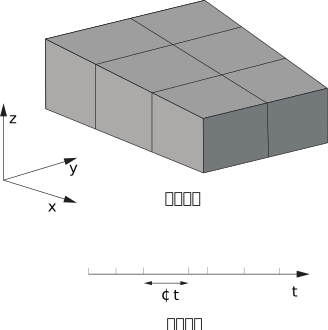
\includegraphics{fig-2-1}
 \caption{解析領域の離散化}
 \label{fig:2.1}
\end{figure}


\begin{figure}[ht]
 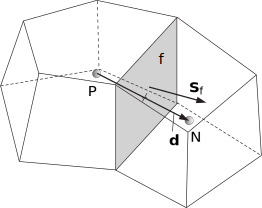
\includegraphics{fig-2-2}
 \caption{有限体積法の離散化におけるパラメータ}
 \label{fig:2.2}
\end{figure}


従属変数とその他の物理量は,たいていセル中心$P$で保存されますが,
面や点で保存される場合もあります.
セルは,一般に$f$とラベル付けされる平らな面で境界付けられます.
OpenFOAMでは,各セルをつくる面の数に制限はなく,
各面の配置にも制約はありません.
このような種類のメッシュは通常,
セルの面が所定の(例えば座標軸に沿った)配置になるメッシュと区別して,
「任意非構造」とよばれます.
任意非構造メッシュを採用したコードは,
領域の形状が複雑であったり時間変化する場合などは特に,
とても自由にメッシュの生成や操作を行うことができます.

ほとんどの物理量はセル中心で定義されますが,
セルの面で定義されるものもいくつかあります.
セルの面には二つのタイプがあります.
\begin{description}
 \item[内部面] 二つのセル(二つを上回ることはありません)をつなぐ面です.
            それぞれの内部面について,OpenFOAMは
            隣接するセルのうち一つをその面の「所有セル」,
            もう一方を「隣接セル」として指定します.
 \item[境界面] 一つだけのセルに属する面で,それゆえ領域の境界と一致します.
            これらの面には単純に所有セルしかありません.
\end{description}


\subsection{OpenFOAMにおけるメッシュ定義}
\label{ssec:2.3.1}
OpenFOAMにはいくつかの異なるレベルのメッシュ記述方法がありますが,
まずはもっとも基本的なメッシュクラスである\OFclass{polyMesh}について述べます.
多面体からなるので\OFclass{polyMesh}といいます.
\OFclass{polyMesh}は以下および\autoref{fig:2.2}に示すように,
メッシュ形状を定義するための最小限の情報で構成されます.
\begin{description}
 \item[点] 頂点の座標ベクトルのリスト,すなわち\OFclass{vectorField}ですが,
            改めて\texttt{typedef}宣言により\OFclass{pointField}と名付けられています.
 \item[面] セルの面のリスト\OFclass{List<face>},あるいは\OFclass{faceList}です.
            ここで,\OFclass{face}クラスは
            \OFclass{pointField}に対応する頂点番号のリストで定義されます.
 \item[セル] セルのリスト\OFclass{List<cell>}あるいは\OFclass{cellList}です.
            ここで,\OFclass{cell}クラスは
            上記の\OFclass{faceList}に対応する面番号のリストで定義されます.
 \item[境界] \OFclass{polyBoundaryMesh}は,境界の異なる領域を表すパッチのリスト
            \OFclass{polyPatchList}から成り立っています.
            このような方法で,解析の際に各々のパッチに
            異なる境界条件を適用できるように境界が細分化されます.
            あらゆる\OFclass{polyPatch}の全ての面は
            \OFclass{faceList}の一つのブロックに保存されており,
            ブロックの最初と最後の面への参照が保存された
            \OFclass{slice}クラスを使うことにより,
            それらの面に簡単にアクセスできます.
            それぞれの\OFclass{polyPatch}は以下から成り立っています.
            \begin{itemize}
             \item \OFclass{slice}
             \item 名前を付けるための\OFclass{word}
            \end{itemize}
\end{description}

有限体積法による離散化には,
\OFclass{polyMesh}に保存されている
メッシュ形状に由来する固有のデータが使われます.
そのためOpenFOAMでは,\OFclass{polyMesh}クラスを拡張した\OFclass{fvMesh}に,
有限体積法による離散化に必要な追加のデータが保存されます.
\OFclass{fvMesh}は{polyMesh}から構成され,
\autoref{tbl:2.1}に示すようなデータが保存されます.
これらのデータは,メッシュが動いたり細分化されたりする場合には,
実行時に更新することができます.


\begin{figure}[ht]
 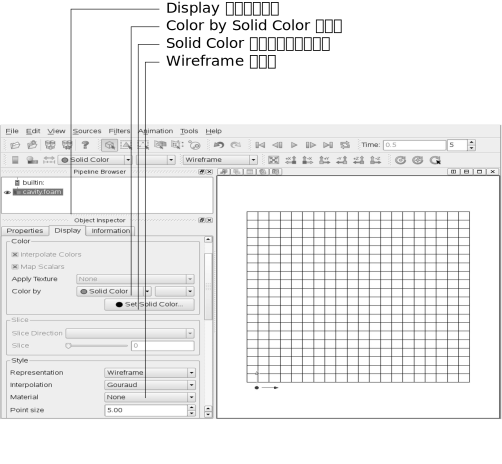
\includegraphics{fig-2-3}
 \caption{OpenFOAMにおける基本的なメッシュ表現の概略図}
 \label{fig:2.3}
\end{figure}


\begin{table}[ht]
 %#! uplatex ProgrammersGuideJa
\begin{tabular}{|c|c|c|c|}
 \hline
 \tblstrut
 クラス & 説明 & 記号 & アクセス関数 \\
 \hline\hline
 \tblstrut
 \OFclass{volScalarField} & セル体積 & $V$ & \verb|V()| \\
 \OFclass{surfaceVectorField} & 面の面積ベクトル & $\bm{S}_{\mathrm{f}}$ & \verb|Sf()| \\
 \OFclass{surfaceScalarField} & 面の面積の絶対値 & $|\bm{S}_{\mathrm{f}}|$ & \verb|magSf()| \\
 \OFclass{volVectorField} & セル中心 & $\bm{C}$ & \verb|C()| \\
 \OFclass{surfaceVectorField} & 面中心 & $\bm{C}_{\mathrm{f}}$ & \verb|Cf()| \\
 \OFclass{surfaceScalarField} & 面の運動流束 ** & $\phi_{\mathrm{g}}$ & \verb|phi()| \\
 \hline
\end{tabular}

 \caption{\OFclass{fvMesh}に保存されるデータ}
 \label{tbl:2.1}
\end{table}


\subsection{OpenFOAMにおける\OFclass{geometricField}の定義}
\label{ssec:2.3.2}
これまでのところ,場,すなわちテンソルのリスト,およびメッシュが定義できます.
これらを合わせることで,領域の離散点におけるテンソル場を定義することができます.
これはOpenFOAMにおいては,テンプレートクラス
\OFclass{geometricField<Type>}によって記述されます.
\OFclass{Field}の値は,
領域内部において例えばセル中心で定義されるものと,
領域の境界において例えば境界面上で定義されるものに分けられます.
\OFclass{geometricField<Type>}は以下のような情報を保存します.
\begin{description}
 \item[内部場] 単純に,\autoref{ssec:2.2.1}で述べたような
            \OFclass{Field<Type>}です.
 \item[境界場] これは\OFclass{GeometricBoundaryField}であり,その中では,
            それぞれのパッチの面について\OFclass{Field}が定義され,
            その境界のパッチについて\OFclass{Field}が定義されます.
            つまりこれは\OFclass{FieldField<Type>}クラスのオブジェクトに保存される,場の場です.
            また\OFclass{fvBoundaryMesh}への参照も保存されます.[**]
 \item[メッシュ] \OFclass{fvMesh}への参照ですが,
            その場がセル中心,面,などのうちどこで定義されているかに応じた
            いくつかの詳細情報も加わります.
 \item[次元] \href{../UserGuideJa/UserGuideJa.pdf#subsection.4.2.6}{ユーザガイドの4.2.6項}で述べる
            \OFclass{dimensionSet}です.
 \item[古い値] 時間微分の離散化には,前の時間ステップにおける場のデータが必要になります.
            \OFclass{geometricField<Type>}は,
            前の,一つ古い時間ステップ,および必要ならばその前の,二つ古い時間ステップ
            において保存された場のデータへの参照を保存しています.
 \item[前回の反復時の値] 反復解法の手順では不足緩和を利用できますが,
            これは前回の反復時のデータへのアクセスを必要とします.
            ここでも,必要であれば,\OFclass{geometricField<Type>}は
            前回の反復時のデータへの参照を保存します.
\end{description}
\autoref{sec:2.3}で述べたように,物理量はセル中心で定義することが主ですが,
セル面上で保存することもよくあり,セル頂点で定義することもときどきあります.
\OFclass{geometricField<Type>}は,場の変数がどこで定義されているかによって,
以下のように\texttt{typedef}宣言で改名されています.
\begin{description}
 \item[\OFclass{volField<Type>}] 場がセル中心で定義されているとき
 \item[\OFclass{surfaceField<Type>}] 場がセルの面で定義されているとき
 \item[\OFclass{pointField<Type>}] 場がセルの頂点で定義されているとき
\end{description}

これらの\OFclass{geometricField<Type>}から
\texttt{typedef}された場のクラスは\autoref{fig:2.4}に図示されています.
\OFclass{geometricField<Type>}は\OFclass{Field<Type>}のテンソル代数を全て継承しており,
全ての演算は\OFclass{dimensionSet}の次元チェックに従います.
また次節で述べる有限体積法の離散化手順にも依存することがあります.
\OFclass{geometricField<Type>}を作るときに使われるクラス構造は\autoref{fig:2.5}%
\footnote{この図はクラス階層を厳密に表したものではなく,
むしろいくつかの原始クラスを\OFclass{geometricField<Type>}につながる
一般的な構造を表したものです.}%
に図示されています.


\begin{figure}[ht]
 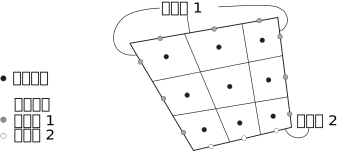
\includegraphics{fig-2-4-a}\par
 \medskip
 (a) \OFclass{volField<Type>}\par
 \bigskip
 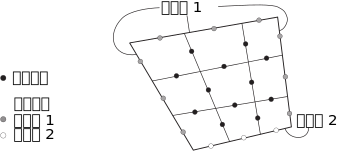
\includegraphics{fig-2-4-b}\par
 \medskip
 (b) \OFclass{surfaceField<Type>}\par
 \bigskip
 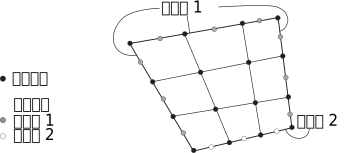
\includegraphics{fig-2-4-c}\par
 \medskip
 (c) \OFclass{pointField<Type>}\par
 \medskip
 \caption{二つの境界パッチをもつメッシュ上で定義された
 \OFclass{geometricField<Type>}のタイプ(簡単のため2次元で表している)}
 \label{fig:2.4}
\end{figure}


\begin{figure}[ht]
 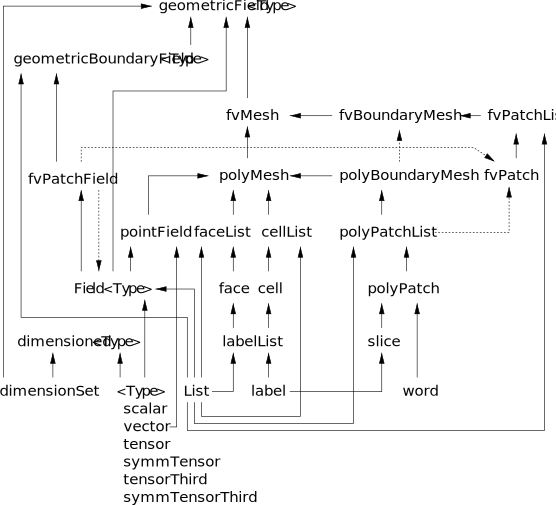
\includegraphics{fig-2-5}
 \caption{\OFclass{geometricField<Type>}につながる基本的なクラス構造}
 \label{fig:2.5}
\end{figure}


\section{方程式の離散化}
\label{sec:2.4}
方程式の離散化により,偏微分方程式は一般に以下のような行列で表される代数方程式に変換されます.
\begin{align}
 \label{eq:2.12}
 [A][x] = [b]
\end{align}
ここで$[A]$は正方行列,$[x]$は従属変数の列ベクトル,$[b]$はソースベクトルです.
$[x]$と$[b]$は,その形状,例えば\OFclass{geometricField<Type>},
またはもっと厳密には,有限体積法による離散化を用いているならば\OFclass{volField<Type>}の
各位置で定義された値のリストという本来の正確な表現ではなく,
むしろ行列用語でいう「ベクトル」です.

$[A]$は代数式群の係数のリストであり,\OFclass{geometricField<Type>}では記述できません.
したがって,独自のクラス\OFclass{fvMatrix}で与えられます.
\OFclass{fvMatrix<Type>}は\OFclass{geometric<Type>Field}の離散化によって生成され,
したがって\OFclass{<Type>}を継承します.
これは,加算\hskip\xkanjiskip\verb|+|,
減算\hskip\xkanjiskip\verb|-|\hskip\xkanjiskip
そして乗算\hskip\xkanjiskip\verb|*|\hskip\xkanjiskip
という標準的な行列の代数演算の多くをサポートします.

OpenFOAMのコードにおいて偏微分方程式の各項は,
それぞれ静的な関数のクラス\OFclass{finiteVolumeMethod}や
\OFclass{finiteVolumeCalculus}を用いて記述されます.
これらのクラスは\texttt{typedef}によって,それぞれ\OFclass{fvm}および\OFclass{fvc}と略されます.
\OFclass{fvm}や\OFclass{fvc}は,
例えば$\nabla^{2}$,$\nabla \inProd {}$および$\partial/\partial t$といった
\OFclass{geometricField<Type>}を離散化する微分演算子を表す静的な関数を備えています.
これらの関数を,一つではなく二つのクラス\OFclass{fvm}と\OFclass{fvc}で定義しているのは,
以下のように区別するためです.
\begin{itemize}
 \item \OFclass{fvm}の関数は陰的な微分を計算し,\OFclass{fvMatrix<Type>}を返す.
 \item \OFclass{fvc}のいくつかの関数は陽的な微分を計算,その他は陽的な計算をし,
       \OFclass{geometricField<Type>}を返す.
\end{itemize}
\autoref{fig:2.6}には,
二つの境界パッチをもつメッシュ上で定義された\OFclass{geometricField<Type>}を示しており,
陽的な演算が単にある場を他の場に変換するだけであることを表しています.
簡単のために2次元で描いています.


\begin{figure}[ht]
 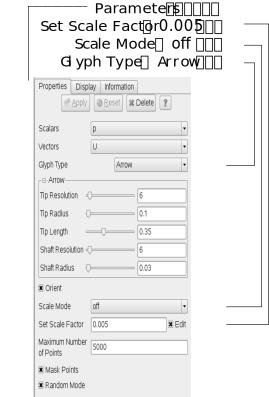
\includegraphics{fig-2-6}
 \caption{\OFclass{geometricField<Type>}とその演算}
 \label{fig:2.6}
\end{figure}


\OFclass{fvm}および\OFclass{fvc}で使える,偏微分方程式の項を離散化する主な関数を
\autoref{tbl:2.2}にリストアップしています.
各項の有限体積法による離散化は,ガウスの定理により,
その体積を囲んでいるセル表面の面積分に変換されます.
\begin{align}
 \label{eq:2.13}
 \int_{V}\nabla \star \phi\,\mathrm{d}V
 = \int_{S}\mathrm{d}\bm{S} \star \phi
\end{align}
ここで$\bm{S}$は表面積ベクトル,$\phi$は任意のテンソル場,
そして$\star$はテンソル任意の乗算,例えば内積,外積,クロス積,
およびそれぞれの微分,発散$\nabla \inProd \phi$,
勾配$\nabla\phi$および$\nabla \times \phi$を表しています.
次に,体積および面積分は各項について後述するような適切なスキームで線形化されます.
OpenFOAMでは,いくつかの項は常に同じスキームで離散化されますが,
その他の項の離散化についてはスキームの選択肢が提供されています.
スキームの選択はコードの中で直接指定することもできますし,
ジョブの実行時にインプットファイルから読み込んで
\OFclass{fvSchemes}クラスのオブジェクトとして保持する方法もあります.


\begin{table}[ht]
 %#! platex ProgrammersGuideJa
\begin{tabular}{|cccc|}
 \hline
 項の記述 & 陰的・陽的 & 記述 & \OFclass{fvm::}または\OFclass{fvc::}の関数 \\
 \hline\hline
 ラプラシアン & 陰的・陽的 & $\nabla^{2}\phi$ & \texttt{laplacian(phi)} \\
 &  & $\nabla \inProd \varGamma \nabla \phi$ & \texttt{laplacian(Gamma, phi)} \\
 \hline
 時間微分 & 陰的・陽的 & $\frac{\partial\phi}{\partial t}$ & \texttt{ddt(phi)} \\
 &  & $\frac{\partial\rho\phi}{\partial t}$ & \texttt{ddt(rho, phi)} \\
 \hline
 時間の2階微分 & 陰的・陽的 & $\frac{\partial}{\partial t}\left(\rho\frac{\partial\phi}{\partial t}\right)$ & \texttt{d2dt2(rho, phi)} \\
 \hline
 移流 & 陰的・陽的 & $\nabla \inProd (\psi)$ & \verb|div(psi, scheme)*| \\
 &  & $\nabla \inProd (\psi\phi)$ & \verb|div(psi, phi, word)*| \\
 &  &  & \verb|div(psi, phi)| \\
 \hline
 発散 & 陽的 & $\nabla \inProd \chi$ & \texttt{div(chi)} \\
 \hline
 勾配 & 陽的 & $\nabla \chi$ & \texttt{grad(chi)} \\
 &  & $\nabla \phi$ & \texttt{gGrad(phi)} \\
 &  &  & \texttt{lsGrad(phi)} \\
 &  &  & \texttt{snGrad(phi)} \\
 &  &  & \texttt{snGradCorrection(phi)} \\
 \hline
 勾配の勾配の二乗 & 陽的 & $|\nabla\nabla\phi|^{2}$ & \texttt{sqrGradGrad(phi)} \\
 \hline
 回転 & 陽的 & $\nabla \times \phi$ & \texttt{curl(phi)} \\
 \hline
 湧き出し & 陰的 & $\rho\phi$ & \texttt{Sp(rho, phi)} \\
 & 陰的・陽的\textsuperscript{\dag} &  & \texttt{SuSp(rho, phi)} \\
 \hline
 \multicolumn{4}{l}{\dag\ 湧き出し\OFkeyword{fvm::SuSp}は
 \OFkeyword{rho}の符号に依存して,陰的または陽的に離散化されます.} \\
 \multicolumn{4}{l}{\dag\ 陽的な湧き出しは単純に
 \OFclass{vol<Type>Field}で指定されます.例:\texttt{rho*phi}} \\
 \multicolumn{4}{l}{関数の引数は以下のようなクラスです.} \\
 \multicolumn{4}{l}{\OFkeyword{phi}: \OFclass{vol<Type>Field}} \\
 \multicolumn{4}{l}{\OFkeyword{Gamma}: \OFclass{scalar},\OFclass{volScalarField},
 \OFclass{volTensorField},\OFclass{surfaceTensorField}.} \\
 \multicolumn{4}{l}{\OFkeyword{rho}: \OFclass{scalar},\OFclass{volScalarField}} \\
 \multicolumn{4}{l}{\OFkeyword{psi}: \OFclass{surfaceTensorField}} \\
 \multicolumn{4}{l}{\OFkeyword{chi}: \OFclass{surface<Type>Field},\OFclass{vol<Type>Field}} \\
\end{tabular}

 \caption{OpenFOAMにおける偏微分方程式の項の離散化}
 \label{tbl:2.2}
\end{table}


\subsection{ラプラシアン項}
\label{ssec:2.4.1}
ラプラシアンの項は,以下のように検査体積で積分・線形化されます.
\begin{align}
 \label{eq:2.14}
 \int_{V}\nabla \inProd (\varGamma\nabla\phi)\,\mathrm{d}V
 = \int_{S}\mathrm{d}\bm{S} \inProd (\varGamma\nabla\phi)
 = \sum_{f}\varGamma_{f}\bm{S}_{f} \inProd (\nabla\phi)_{f}
\end{align}
みているセル$P$の中心と隣のセル$N$の中心の間の長さベクトル$\bm{d}$が
そのフェイス面に垂直,すなわち$\bm{S}_{f}$に平行ならば,
面の勾配の離散化は陰的になります.
\begin{align}
 \label{eq:2.15}
 \bm{S}_{f} \inProd (\nabla\phi)_{f}
 = |S_{f}|\frac{\phi_{N} - \phi_{P}}{|\bm{d}|}
\end{align}
非直交メッシュの場合,
セル中心勾配(これはセル中心値の中心差分から計算される)の
内挿によって評価される陽的な項が加わります.


\subsection{対流項}
\label{ssec:2.4.2}
対流項は,以下のように検査体積で積分・線形化されます.
\begin{align}
 \label{eq:2.16}
 \int_{V}\nabla \inProd (\rho\bm{U}\phi)\,\mathrm{d}V
 = \int_{S}\mathrm{d}\bm{S} \inProd (\rho\bm{U}\phi)
 = \sum_{f}\bm{S}_{f} \inProd (\rho\bm{U})_{f}\phi_{f}
 = \sum_{f}F\phi_{f}
\end{align}

表面の場$\phi_{f}$はさまざまなスキームで評価されます.
\begin{description}
 \item[中心差分 (CD)] は,2次精度ですが不安定です.
            \begin{align}
             \label{eq:2.17}
             \phi_{f} = f{x}\phi_{P} + (1 - f_{x})\phi_{N}
            \end{align}
            ここで$f_{x} \equiv \overline{fN}/\overline{PN}$,
            $\overline{fN}$は$f$とセル中心$N$の距離,
            $\overline{PN}$はセル中心同士$P$と$N$の距離です.
 \item[風上差分 (UD)] は,流れの方向から$\phi_{f}$を決定し,
            精度は犠牲になりますが安定です.
            \begin{align}
             \label{eq:2.18}
             \phi_{f} =
             \begin{cases}
              \phi_{P} & F \ge 0 \text{のとき} \\
              \phi_{N} & F < 0 \text{のとき}
             \end{cases}
            \end{align}
 \item[ブレンド差分 (BD)] スキームは,適切な精度で
            安定性を保つことを狙ってUDとCDを組み合わせます.
            \begin{align}
             \phi_{f} = (1 - \gamma)(\phi_{f})_{\mathrm{UD}} + \gamma(\phi_{f})_{\mathrm{CD}}
            \end{align}
            OpenFOAMには,ブレンド係数$\gamma$を選ぶGamma差分スキームのいくつかの実装がありますが,
            それはほかのよく知られたスキーム,van Leer,SUPERBEE,MINMODなどを表しています.
\end{description}


\subsection{1階の時間微分}
\label{ssec:2.4.3}
1階の時間微分$\partial/\partial t$は,以下のように検査体積で積分されます.
\begin{align}
 \label{eq:2.20}
 \frac{\partial}{\partial t}\int_{V}\rho\phi\,\mathrm{d}V
\end{align}
この項は,以下のものを使って時間に関して単純な差分で離散化されます.
\begin{description}
 \item[新しい値] いま解いている時間ステップの値$\phi^{n} \equiv \phi(t + \Delta t)$
 \item[古い値] 前の時間ステップで保存された値$\phi^{o} \equiv \phi(t)$
 \item[二つ古い値] 二つ前の時間ステップで保存された値$\phi^{oo} \equiv \phi(t - \Delta t)$
\end{description}
\href{../UserGuideJa/UserGuideJa.pdf#section.4.4}{ユーザガイドの4.4節}に詳しく述べられているように,
該当する入力ファイルの中で\OFkeyword{timeScheme}キーワードを使って,
二つのうち一つの離散化スキームを宣言することができます.
\begin{description}
 \item[オイラーの陰解法] スキーム,\OFkeyword{timeScheme EulerImplicit},
            これは時間に関して1次精度です.
            \begin{align}
             \label{eq:2.21}
             \frac{\partial}{\partial t}\int_{V}\rho\phi\,\mathrm{d}V
             = \frac{(\rho_{P}\phi_{P}V)^{n} - (\rho_{P}\phi_{P}V)^{o}}{\Delta t}
            \end{align}
 \item[後退差分] スキーム,\OFkeyword{timeScheme BackwardDifferencing},
            これは二つ前の値を保存することにより時間に関して2次精度であり,
            したがって\OFkeyword{EulerImplicit}よりデータ保存のオーバーヘッドが大きくなります.
            \begin{align}
             \label{eq:2.22}
             \frac{\partial}{\partial t}\int_{V}\rho\phi\,\mathrm{d}V
             = \frac{3(\rho_{P}\phi_{P}V)^{n} - 4(\rho_{P}\phi_{P}V)^{o}
             + (\rho_{P}\phi_{P}V)^{oo}}{2\Delta t}
            \end{align}
\end{description}


\subsection{2階の時間微分}
\label{ssec:2.4.4}
2階の時間微分は,以下のように検査体積で積分・線形化されます.
\begin{align}
 \label{eq:2.23}
 \frac{\partial}{\partial t}\int_{V}\rho\frac{\partial\phi}{\partial t}\,\mathrm{d}V
 = \frac{(\rho_{P}\phi_{P}V)^{n} - 2(\rho_{P}\phi_{P}V)^{o}
 + (\rho_{P}\phi_{P}V)^{oo}}{\Delta t^{2}}
\end{align}
これは時間について1次精度です.


\subsection{発散}
\label{ssec:2.4.5}
この節で述べる発散項は,
\autoref{ssec:2.4.2}の対流項とは区別される完全に陽的な項です.
つまり対流項は,速度とある従属変数の積の発散ではありません.
この項は以下のように検査体積で積分・線形化されます.
\begin{align}
 \label{eq:2.24}
 \int_{V}\nabla \inProd \phi\,\mathrm{d}V
 = \int_{S}\mathrm{d}\bm{S} \inProd \phi
 = \sum_{f}\bm{S}_{f} \inProd \phi_{f}
\end{align}
\OFkeyword{fvc::div}関数は\OFclass{surface<Type>}または
\OFclass{vol<Type>Field}のどちらも引数にとることができます.
前者では$\phi_{f}$は直接与えられ,
後者では\autoref{ssec:2.4.10}で述べる中心差分で値が面上に内挿されます.


\subsection{勾配}
\label{ssec:2.4.6}
勾配の項は様々な方法で評価できる陽的な項です.
そのスキームは,例えば\OFkeyword{fvc::gGrad},\OFkeyword{fvc::lsGrad}などのような
離散化スキームに対して適切な特定の勾配関数を選ぶか,
または入力ファイルの中の適切な\OFkeyword{timeScheme}キーワードに
連動した\OFkeyword{fvc::grad}関数を使うか,
いずれの方法でも評価できます.
\begin{description}
 \item[ガウス積分] は,\OFkeyword{fvc::grad}関数を
            \OFkeyword{timeScheme Gauss}と合わせて使うことで動作します.
            この離散化は体積分に対してガウスの定理を適用する標準的な手法を使います.
            \begin{align}
             \label{eq:2.25}
             \int_{V}\nabla\phi\,\mathrm{d}V
             = \int_{S}\mathrm{d}\bm{S}\phi
             = \sum_{f}\bm{S}_{f}\phi_{f}
            \end{align}
 \item[最小二乗法] は,以下の考えに基づいています.
            \begin{enumerate}
             \item 点$P$における値を,点$P$における勾配を使って隣の点$N$に外挿する.
             \item 点$N$に外挿された値を,点$N$における実際の値と比較,この差が誤差となる.
             \item 点$P$の付近の全ての点における誤差を,
                   それぞれの勾配で重み付けして二乗した総和を最小化すれば,
                   勾配の良い近似値が得られる.
            \end{enumerate}
            最小二乗法は\OFkeyword{fvc::grad}関数を
            \OFkeyword{timeScheme leastSquares}と組み合わせるか,
            直接\OFkeyword{fvc::lsGrad}を使うことで動作します.
            この離散化は,まず全ての点$P$において,その近隣の点$N$での総和を求めて,
            テンソル$\bm{G}$を計算します.
            \begin{align}
             \label{eq:2.26}
             \bm{G} = \sum_{N}w_{N}^{2}\bm{d}\bm{d}
            \end{align}
            ここで$\bm{d}$は$P$から$N$へのベクトルであり,
            重み関数は$w_{N} = 1/|\bm{d}|$です.
            勾配は以下のように評価されます.
            \begin{align}
             \label{eq:2.27}
             (\nabla\phi)_{P}
             = \sum_{N}w_{N}^{2}\bm{G}^{-1} \inProd \bm{d}(\phi_{N} - \phi_{P})
            \end{align}
 \item[面に垂直な勾配] 面に垂直な勾配$\bm{n}_{f} \inProd (\nabla\phi)_{f}$は
            セルの面において以下のスキームを使って評価できます.
            \begin{align}
             \label{eq:2.28}
             (\nabla\phi)_{f} = \frac{\phi_{N} - \phi_{P}}{|\bm{d}|}
            \end{align}
            この勾配は\OFkeyword{fvc::snGrad}関数で呼び出され,
            \OFclass{surfaceField<Type>}を返します.
            このスキームは\autoref{ssec:2.4.1}で述べた
            ラプラシアンの離散化スキームと似た方法で直接評価され,
            また同じように非直交メッシュの場合には,
            この面の勾配の精度を高めるために補正が加えられます.
            この補正は\OFkeyword{fvc::snGradCorrection}関数を使って呼び出されます.
            [Check**]
\end{description}


\subsection{勾配の勾配の平方}
\label{ssec:2.4.7}
勾配の勾配の平方の項は,場の勾配をとり,得られた勾配場の勾配をとり,
そしてその結果の絶対値二乗を計算することで評価されます.
$\phi$の勾配の勾配の平方を数式で書くと$|\nabla (\nabla\phi)|^{2}$となります.


\subsection{回転}
\label{ssec:2.4.8}
回転は,\autoref{ssec:2.4.6}で述べた勾配の項から評価されます.
まず勾配が離散化され,それから\autoref{eq:2.7}の関係(以下に再掲)を
使って回転が評価されます.
\begin{align*}
 \nabla \times \phi = 2 \mathop{*} (\mathop{\mathrm{skew}}\nabla\phi)
\end{align*}


\subsection{湧き出し項}
\label{ssec:2.4.9}
湧き出し項は三つの方法で指定できます.
\begin{description}
 \item[陽解法] すべての陽的な項は\OFclass{volField<Type>}です.
            したがって,陽的な湧き出し項は単純に値の場として等式の中に組み込まれます.
            例えば,\OFkeyword{phi}と\OFkeyword{f}を\OFclass{volScalarField}として定義し,
            そして以下のようにします.
            \begin{OFverbatim}[file]
solve(fvm::laplacian(phi) == f)
            \end{OFverbatim}
 \item[陰解法] 陰的な湧き出し項は,以下のように検査体積で積分・線形化されます.
            \begin{align}
             \label{eq:2.29}
             \int_{V}\rho\phi\,\mathrm{d}V = \rho_{P}V_{P}\phi_{P}
            \end{align}
 \item[陰・陽解法] 陰的な湧き出し項は,行列の対角成分の係数を変えます.
            その係数と行列の項の符号に依存して,
            これは行列の対角成分の支配力を増大または減少させます.
            対角成分の支配力を減少させることは,
            行列の方程式の反復解法の際の不安定さを引き起こします.
            したがって,OpenFOAMは混成の湧き出し項の離散化方法を提供しており,
            これは係数が正のとき陰的に,負のときには陽的になります.
            数式上は,点$P$に対する行列の係数は$V_{P}\max(\rho_{P},\ 0)$,
            そして湧き出し項は$V_{P}\phi_{P}\min(\rho_{P},\ 0)$となります.
\end{description}


\subsection{その他の陽的な離散化スキーム}
\label{ssec:2.4.10}

他にも\OFclass{volField<Type>}を\OFclass{surface<Type>Field}に,
および逆に変換する離散化手法がいくつかあります.
\begin{description}
 \item[面積分] \OFkeyword{fvc::surfaceIntegrate}は,
            それぞれのセルを区切る面での値\OFclass{surface<Type>Field}の総和をとり,
            セルの体積で割るという操作をします.
            すなわち$(\sum_{f}\phi_{f})/V_{P}$となります.
            これは\OFclass{volField<Type>}を返します.
 \item[面総和] \OFkeyword{fvc::surfaceSum}は,
            それぞれのセルを区切る面での値\OFclass{surface<Type>Field}の総和をとる操作です.
            すなわち$\sum_{f}\phi_{f}$となり,
            \OFclass{volField<Type>}を返します.
 \item[平均値] \OFkeyword{fvc::average}は,
            面の値\OFclass{surface<Type>Field}の面積重み付け平均をとります.
            すなわち$(\sum_{f}S_{f}\phi_{f})/\sum_{f}S_{f}$となり,
            \OFclass{volField<Type>}を返します.
 % \item[Reconstruct] 
 \item[面内挿] \OFclass{geometric<Type>Field}の関数\OFkeyword{faceInterpolate()}は,
            セル中心の値\OFclass{volField<Type>}を,
            中心差分を使ってセルの面上へ内挿し,\OFclass{surface<Type>Field}を返します.
\end{description}



\section{時間微分}
\label{sec:2.5}
時間微分の離散化については\autoref{ssec:2.4.3}および\autoref{ssec:2.4.4}で述べましたが,
非定常問題における空間微分の扱い方について考える必要があります.
もし$\mathcal{A}$を任意の空間微分演算子,
例えばラプラシアン,として,
あらゆる空間微分を$\mathcal{A}\phi$で表すとすれば,
非定常の偏微分方程式を積分型で以下のように表記できます.
\begin{align}
 \label{eq:2.30}
 \int_{t}^{t + \Delta t}\left[\frac{\partial}{\partial t}\int_{V}\rho\phi\,\mathrm{d}V
 + \int_{V}\mathcal{A}\phi\,\mathrm{d}V\right]\mathrm{d}t = 0
\end{align}
\autoref{eq:2.21}のオイラー陰解法を使うと,第1項は次のように書けます.
\begin{align}
 \label{eq:2.31}
 \int_{t}^{t + \Delta t}
 \left[\frac{\partial}{\partial t}\int_{V}\rho\phi\,\mathrm{d}V\right]\mathrm{d}t
 &= \int_{t}^{t + \Delta t}
 \frac{(\rho_{P}\phi_{P}V)^{n} - (\rho_{P}\phi_{P}V)^{o}}{\Delta t}\mathrm{d}t \\
 &= \frac{(\rho_{P}\phi_{P}V)^{n} - (\rho_{P}\phi_{P}V)^{o}}{\Delta t}\Delta t
\end{align}

第2項は次のように書けます.
\begin{align}
 \label{eq:2.32}
 \int_{t}^{t + \Delta t}\left[\int_{V}\mathcal{A}\phi\,\mathrm{d}V\right]\mathrm{d}t
 = \int_{t}^{t + \Delta t}\mathcal{A}^{*}\phi\,\mathrm{d}t
\end{align}
ここで$\mathcal{A}^{*}$は空間で離散化した$\mathcal{A}$を表します.
時間積分は三つの方法で離散化できます.
\begin{description}
 \item[オイラー陰解法] 空間については陰解法で離散化し,したがって現在の値$\phi^{n}$をとります.
            \begin{align}
             \label{eq:2.33}
             \int_{t}^{t + \Delta t}\mathcal{A}^{*}\phi\,\mathrm{d}t
             = \mathcal{A}^{*}\phi^{n}\Delta t
            \end{align}
            これは時間について1次精度であり,有界性と無条件安定性を保証します.
 \item[陽解法] 空間については陽解法で離散化し,したがって前の時刻の値$\phi^{o}$をとります.
            \begin{align}
             \label{eq:2.34}
             \int_{t}^{t + \Delta t}\mathcal{A}^{*}\phi\,\mathrm{d}t
             = \mathcal{A}^{*}\phi^{o}\Delta t
            \end{align}
            これは時間について1次精度であり,もしクーラン数$\nCo$が$1$より大きければ不安定です.
            クーラン数は以下のように定義されます.
            \begin{align}
             \label{eq:2.35}
             \nCo = \frac{\bm{U}_{f} \inProd \bm{d}}{|\bm{d}|^{2}\Delta t}
            \end{align}
            ここで$\bm{U}_{f}$は代表速度,例えば波面の速度,流れの速度などです.
 \item[クランク・ニコルソン法] 空間の項の離散化に台形公式を使い,
            したがって現在の値$\phi^{n}$と前の時刻の値$\phi^{o}$の平均値をとります.
            \begin{align}
             \label{eq:2.36}
             \int_{t}^{t + \Delta t}\mathcal{A}^{*}\phi\,\mathrm{d}t
             = \mathcal{A}^{*}\left(\frac{\phi^{n} + \phi^{o}}{2}\right)\Delta t
            \end{align}
            これは時間について2次精度であり,無条件で安定ですが,有界性は保証されません.
\end{description}


\subsection{OpenFOAMにおける時間微分の取扱い}
\label{ssec:2.5.1}
現在のところ,時間の離散化の取り扱いは,
解くべき偏微分方程式における空間微分の実装によって制御されます.
例えば,非定常の拡散方程式を解きたいとします.
\begin{align}
 \label{eq:2.37}
 \frac{\partial\phi}{\partial t} = \kappa\nabla^{2}\phi
\end{align}
これに対するオイラーの陰解法は以下のようになります.
\begin{OFverbatim}[file]
solve(fvm::ddt(phi) == kappa*fvm::laplacian(phi))
\end{OFverbatim}
ここで\OFkeyword{Laplacian}の項を陰解法で離散化するために\OFclass{fvm}クラスを使います.
陽解法で実装するには以下のようにします.
\begin{OFverbatim}[file]
solve(fvm::ddt(phi) == kappa*fvc::laplacian(phi))
\end{OFverbatim}
今度は\OFkeyword{Laplacian}の項を陽解法で離散化するために\OFclass{fvc}クラスを使います.
クランク・ニコルソン・スキームは,陰解法と陽解法の平均をとることで実装できます.
\begin{OFverbatim}[file]
solve
    (
    fvm::ddt(phi)
    ==
    kappa*0.5*(fvm::laplacian(phi) + fvc::laplacian(phi))
    )
\end{OFverbatim}



\section{境界条件}
\label{sec:2.6}
解きたい問題を完成させるためには境界条件が必要です.
したがって全ての境界面において境界条件を指定しなければなりません.
境界条件は二つのタイプに分けられます.
\begin{description}
 \item[ディリクレ条件] は,その従属変数の境界における値を定めます.
            したがって,このガイドでは「固定値」とよびます.
            % したがって,このガイドでは `fixed value' とよびます.
 \item[ノイマン条件] は,その従属変数の境界に垂直な勾配を定めます.
            したがって,このガイドでは「固定勾配」とよびます.
            % したがって,このガイドでは `fixed gradient' とよびます.
\end{description}

面にわたる総和$\sum_{f}$を含む項の離散化を行うときには,
それらの面のうちの一つが境界面であったらどうなるかを考慮する必要があります.
\begin{description}
 \item[固定値] 境界における値$\phi_{b}$を指定
            \begin{itemize}
             \item 離散化に,境界面における値$\phi_{f}$を使う場合は,
                   単純に$\phi_{b}$で置き換えることができます.
                   例えば\autoref{eq:2.16}の移流項の場合です.
             \item 面における勾配$(\nabla\phi)_{f}$が必要な項,
                   例えばラプラシアンなど,の場合には,
                   その勾配は境界面における値とセル中心の値を使って計算されます.
                   \begin{align}
                    \label{eq:2.38}
                    \bm{S}_{f} \inProd (\nabla\phi)_{f}
                    = |S_{f}|\frac{\phi_{b} - \phi_{P}}{|\bm{d}|}
                   \end{align}
            \end{itemize}
 \item[固定勾配] 固定勾配境界条件$g_{b}$は,
            勾配と,境界の単位法線ベクトルとの内積になります.
            \begin{align}
             \label{eq:2.39}
             g_{b} = \left(\frac{\bm{S}}{|\bm{S}|} \inProd \nabla\phi\right)_{f}
            \end{align}
            \begin{itemize}
             \item 離散化に,境界面における値$\phi_{f}$を使う場合は,
                   セル中心の値を境界上に内挿する必要があります.
                   \begin{align}
                    \label{eq:2.40}
                    \phi_{f}
                    &= \phi_{P} + \bm{d} \inProd (\nabla\phi)_{f} \notag \\
                    &= \phi_{P} + |\bm{d}|g_{b}
                   \end{align}
             \item 離散化に面の勾配が評価される場合は,
                   直接$g_{b}$で置き換えることができます.
                   \begin{align}
                    \label{eq:2.41}
                    \bm{S}_{f} \inProd (\nabla\phi)_{f} = |S_{f}|g_{b}
                   \end{align}
            \end{itemize}
\end{description}


\subsection{物理的な境界条件}
\label{ssec:2.6.1}
境界条件の指定は通常,本当の振る舞いに対するエンジニアの解釈です.
現実の境界条件は一般に,
前節で述べたような数値的記述ではなく,
物理的な特性によって定義されます.
非圧縮性流体の流れでは,以下のような物理的な境界があります.
\begin{description}
 \item[入口] 入口における速度場が与えられ,それと整合させるために,
            圧力の境界条件は勾配ゼロになります.
 \item[出口] 出口における圧力場が与えられ,
            速度には勾配ゼロ境界条件が指定されます.
 \item[滑りなし不浸透性壁面] 流体の速度は壁面自身の速度と等しくなり,
            したがって,固定値条件が指定されます.
            壁を通り抜ける流束がゼロであることから,
            圧力は勾配ゼロが指定されます.
\end{description}

解の領域と境界条件がある面について対称となるような問題では,
その対称面の片側の半分の領域だけしかモデル化する必要はありません.
その面の境界条件は以下に従って指定しなければなりません.
\begin{description}
 \item[対称面] 対称面条件は,その面に垂直な勾配成分をゼロと指定します.[Check**]
\end{description}

../../../ProgrammersGuideJa/chapter3.tex
../../../UserGuideJa/chapter4.tex
%#! platex UserGuideJa
\chapter{メッシュの生成と変換}
\label{chap:5}
本章では,OpenFOAMにおけるメッシュの生成に関する話題について述べます.
\autoref{sec:5.1}ではOpenFOAMにおいて
メッシュがどのように記述されるか概説します.
\autoref{sec:5.3}では六面体格子ブロックのメッシュの生成を行う
\OFtool{blockMesh}ユーティリティについて説明します.
\autoref{sec:5.4}では三角表面形状から自動的に
六面体格子や分割六面体格子の複雑なメッシュを生成する
\OFtool{snappyHexMesh}ユーティリティについて説明します.
\autoref{sec:5.5}ではサードパーティの製品で生成したメッシュを,
OpenFOAMで読み込むことができるフォーマットに変換する手法もあることを述べます.



\section{メッシュの記法}
\label{sec:5.1}
\index{メッシュ!きほう@記法}%
この節では,OpenFOAMのC++のクラスがどのようにメッシュを扱うか,
その仕様について説明します.
メッシュは数値解析において不可欠のものであり,
妥当で精密な解を得るためには一定の条件を満している必要があります.
OpenFOAMは,実行時,メッシュが妥当かどうかの一連の条件を満しているか
厳しくチェックし,もしその条件を満していない場合には,実行を止めます.
このためOpenFOAMが実行する前に,
サードパーティ製のメッシャで生成した大規模なメッシュを
修正することに疲れてしまうかもしれません.
OpenFOAM上で受けいれられるようにするために,
根気良く修正する羽目に陥いることがあります.
それは残念なことではありますが,
メッシュの妥当性のチェックを行わなかったら,
計算が始まる前に解は発散してしまうこともあるわけですから,
OpenFOAMがメッシュの妥当性を常にチェックすることは決して悪いことではありません.

通常,OpenFOAMは,任意の多角形の面に囲まれた3次元で定義される
任意の多面体セルによってメッシュを定義しますので,
セルの面の数は無制限であり,その面についても,
辺の数は無制限で配列についても何の制約もありません.
このような汎用性が高いメッシュをOpenFOAMでは
\index{polyMesh@\OFclass{polyMesh}!クラス}%
\index{クラス!polyMesh@\OFclass{polyMesh}}%
\OFclass{polyMesh}と定義しています.
プログラマ・ガイドの2.3節においてより詳細に述べますが,
このような形式のメッシュを用いていると,
特に計算領域の幾何形状が複雑であったり,それらが何度も変更されるときに,
メッシュの生成やその操作においてとても大きな自由度があることだけを,
ここでは述べておくことにします.
しかしながら,このようにメッシュが無条件の汎用性をもった代償として,
従来のツールによって生成されたメッシュを変換するのは難しいこともあります.
そのため,OpenFOAMのライブラリは,
既存のセル形状セットを元にした従来のメッシュのフォーマットを
上手く扱う\OFtool{cellShape}ツールを提供しています.


\subsection{メッシュの仕様と妥当性の制約}
\label{ssec:5.1.1}
\index{メッシュ!しよう@仕様}%
\index{メッシュ!だとうせいのせいやく@妥当性の制約}%
OpenFOAMのメッシュのフォーマットである
\OFclass{polyMesh}や\OFtool{cellShape}ツールを説明する前に,
まず,OpenFOAMにおけるメッシュの妥当性の制約について述べたいと思います.
メッシュが満していなければならない条件とは以下の通りです.

\subsubsection{点}
\label{sssec:5.1.1.1}
点というのは,3次元空間における位置であり,
メートル ($\unit*{m}$) 単位のベクトルによって定義されます.
点の集まりはリストに蓄積され,個々の点はリストにおける位置を表わし,
0から始まるラベルにより参照されます.
この点のリストには,別々の点でありながら位置が全く同一である点や,
一つの面にも属さない点が含まれることはありません.

\subsubsection{面}
\label{sssec:5.1.1.2}
面は点を順番に並べたものであり,
ひとつひとつの点はラベルによって参照されます.
面における点のラベル順は,
隣接した二つの点が一つの辺によって接続されるように付けられるため,
面の周囲をぐるっと廻るように点の番号を追うことになります.
点と同様に,面の集まりはリストで管理され,
個々の面は,リストにおける位置を表わすラベルによって参照されます.
面の法線方向ベクトルの向きは右手の法則により決まります.
すなわち,\autoref{fig:5.1}のように,面に向って見たとき,
点の順序が反時計廻りであったら,法線方向ベクトルはこちらを向いていることになります.


\begin{figure}[ht]
 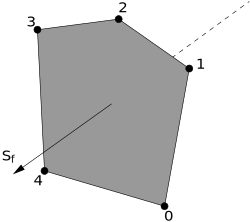
\includegraphics{fig-5-1}
 \caption{面における点の順序から決まる面領域ベクトル}
 \label{fig:5.1}
\end{figure}


面には2種類あります.
\begin{description}
 \item[内部の面]
            これらの面は必ず二つのセルに接続されており,
            その数が2を超えることはありません.
            また,内部の面において,その法線方向ベクトルが,
            より大きなラベルをもつセルに向くように,
            点のラベルの番号付けがなされます.
            つまり,セル2とセル5を接続している面だったら,
            その法線はセル5を向くわけです.
 \item[境界の面]
            これらは領域の境界にあるので,一つのセルにしか属しません.
            したがって,ある境界の面を参照するのは,
            一つのセルと境界パッチだけです.
            点ラベルの番号付けは,
            面の法線が計算領域の外側に向くように設定されます.
\end{description}

\subsubsection{セル}
\label{sssec:5.1.1.3}
セルは,面を任意の順序で並べたものです.セルは以下に示す性質が必ず必要です.
\begin{description}
 \item[切れ目なく連続である]
            セル群は計算領域全体を完全にカバーしており,
            かつ,お互いに重複してはなりません.
 \item[凸である]
            全てのセルは凸で,かつ,
            セル中心はセルの内側にある必要があります.
 \item[閉じている]
            全てのセルは幾何的にも位相的(トポロジ的)にも
            閉じていなければなりません.
            ここで,セルが幾何的に閉じているためには,
            全ての面領域ベクトルがセルの外側を向いているとして,
            それらのベクトル和が,正確にゼロ・ベクトルとなる必要があります.
            また,セルが位相的に閉じているためには,
            問題において,セル中の全ての辺が,
            二つの面により使用されている必要があります.
 \item[直交性がある]
            メッシュ内部の全ての面に対し,中心間ベクトルというのを,
            隣接する二つのセルの中心間を,
            小さいほうのラベルのセル中心から大きいほうのラベルの
            セル中心への向きで結んだベクトルとして定義することができます.
            直交性の制約というのは,内部の全ての面に対し,
            先に述べた面の面積ベクトルと中心間ベクトルのなす角が,
            常に$90\unit*{\degree}$未満であることをいいます.
\end{description}

\subsubsection{境界}
\label{sssec:5.1.1.4}
境界というのはパッチのリスト(集合)であり,
これら一つ一つは,ある境界条件が割り当てられています.
ここで,パッチというのは面のラベルのリストであり,
境界の面のみで形成され,内部の面を含みません.
この境界は閉じていることが条件であるので,
境界における全面領域ベクトルの和は,数値計算上ゼロ・ベクトルになります.


\subsection{\OFclass{polyMesh}の記述}
\label{ssec:5.1.2}
\OFpath{constant}ディレクトリのサブディレクトリである
\OFpath{polyMesh}には,
そのケースの
\index{polyMesh@\OFclass{polyMesh}!クラス}%
\index{クラス!polyMesh@\OFclass{polyMesh}}%
\OFclass{polyMesh}データが全て収められています.
このpolyMeshの記述は面ベースであり,既に述べましたように,
内部のセルは二つのセルと接続し,境界面はセルと境界のパッチを指定します.
各面には「保有」セルと「隣接」セルが割り当てられ,
面を通じた接続は,保有セルと隣接セルのラベルによって
簡潔に記述することができます.
境界の場合には,面に接続されたセルがその面の保有者であり,
隣接セルには$-1$のラベルが割り充てられます.
以上を踏まえた上で,以下のファイルで構成される入出力の詳細をご覧ください.
\begin{description}
 \item[\OFdictionary{points}]
\index{points@\OFdictionary{points}!ディクショナリ}%
\index{ディクショナリ!points@\OFdictionary{points}}%
            セルの頂点を記述するベクトルのリストです.
            ここで,リストにおける最初のベクトルは頂点$0$,
            次のベクトルの頂点$1$という風に番号付けします.
 \item[\OFdictionary{faces}]
\index{faces@\OFdictionary{faces}!ディクショナリ}%
\index{ディクショナリ!faces@\OFdictionary{faces}}%
            面のリストです.各面は点中の頂点の番号のリストで
            成り立ってます.ここで,先程と同様に,
            リスト中の最初の面の番号は$0$です.
 \item[\OFdictionary{owner}]
\index{owner@\OFdictionary{owner}!ディクショナリ}%
\index{ディクショナリ!owner@\OFdictionary{owner}}%
            保有セルのラベルのリストです.
            面のリストと同じ順番に並んでますので,
            リストの最初のラベルは$0$番の面の保有セルのラベル,
            次のラベルは$1$番の面の保有セルのラベルということになります.
 \item[\OFdictionary{neighbour}]
\index{neighbour@\OFdictionary{neighbour}!ディクショナリ}%
\index{ディクショナリ!neighbour@\OFdictionary{neighbour}}%
            隣接セルのラベルのリストです.
 \item[\OFdictionary{boundary}]
\index{boundary@\OFdictionary{boundary}!ディクショナリ}%
\index{ディクショナリ!boundary@\OFdictionary{boundary}}%
            パッチのリストです.以下のように,
            パッチ名の宣言で始まる各パッチに対するディクショナリで構成されます.
\begin{OFverbatim}[file]
movingWall
{
    type patch;
    nFaces 20;
    startFace 760;
}
\end{OFverbatim}
\index{startFace@\OFkeyword{startFace}!キーワード}%
\index{キーワード!startFace@\OFkeyword{startFace}}%
            \OFkeyword{startFace}はそのパッチにおける最初の面のラベル番号です.
            また
\index{nFaces@\OFkeyword{nFaces}!キーワード}%
\index{キーワード!nFaces@\OFkeyword{nFaces}}%
            \OFkeyword{nFaces}は,そのパッチ中の面数です.
\end{description}
備考:計算対象にいくつセルがあるか知りたい場合には,
\OFpath{owner}ファイルの\OFkeyword{FoamFile}ヘッダにおける
\OFkeyword{nCells}を見てください.


\subsection{\OFtool{cellShape}ツール}
\label{ssec:5.1.3}
別の標準的(でより単純)なメッシュ形式を,
OpenFOAMのライブラリで扱えるように変換する際に,
特に必要となるであろう\OFtool{cellShape}というツールについても説明しておきたいと思います.

多くのメッシュ・ジェネレータや後処理システムは,
実際にあり得る多面体セルの形状種類に対し,
その一部だけをサポートするものがほとんどです.
それらは,メッシュをセル形状セットといった,
3次元のセル幾何形状の限られた組み合わせで定義します.
OpenFOAMのライブラリには,
これらの一般的な形状集の定義がありますので,
上記のようなメッシュを先の節で述べたpolyMesh形式に変換することができます.

OpenFOAMによってサポートされるcellShapeモデルを
\autoref{tbl:5.1}に示します.
形状は,形状モデルにおける番号付けスキームに従って付けれらた
頂点ラベルの順序によって定義されます.
点や面,辺に対する番号付けスキームも\autoref{tbl:5.1}に書いてあります.
点の番号付けは,形状がねじれたり,
他の形状に変化することがないようにしなければならないので,
同じ点番号は複数回使用できないことになります.
さらに,重複した点はOpenFOAMでは使う必要はありません.
なぜなら,OpenFOAMで使用可能な形状は,六面体の変種を全てカバーしているからです.

セルの記述は,セルモデルの名前と,
ラベルの順序リストという二つの部分より行います.例えば,以下の点のリストを使うと,
\begin{OFverbatim}[file]
8
    (
        (0 0 0)
        (1 0 0)
        (1 1 0)
        (0 1 0)
        (0 0 0.5)
        (1 0 0.5)
        (1 1 0.5)
        (0 1 0.5)
    )
\end{OFverbatim}
六面体セルは以下のように書けます.
\begin{OFverbatim}[file]
(hex 8(0 1 2 3 4 5 6 7))
\end{OFverbatim}
ここで,六面体セルの形状は\OFkeyword{hex}というキーワードで記述しましたが,
他の形状については,\autoref{tbl:5.1}に示したキーワードを使って記述できます.


\begin{table}[p]
 %#! platex UserGuideJa
\begin{tabular}{llccc}
 セルタイプ & キーワード & 点の番号付け & 面の番号付け & 辺の番号付け \\
 \hline
 \tblstrut
 六面体 & \OFkeyword{hex}
     & 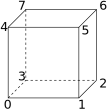
\includegraphics{tbl-5-1-1-v}
         & 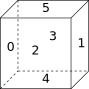
\includegraphics{tbl-5-1-1-f}
             & 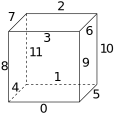
\includegraphics{tbl-5-1-1-e} \\
 くさび形 & \OFkeyword{wedge}
     & 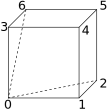
\includegraphics{tbl-5-1-2-v}
         & 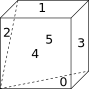
\includegraphics{tbl-5-1-2-f}
             & 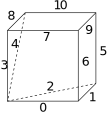
\includegraphics{tbl-5-1-2-e} \\
 三角柱 & \OFkeyword{prism}
     & 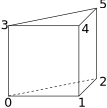
\includegraphics{tbl-5-1-3-v}
         & 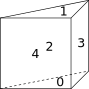
\includegraphics{tbl-5-1-3-f}
             & 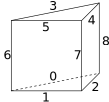
\includegraphics{tbl-5-1-3-e} \\
 四角錐 & \OFkeyword{pyr}
     & 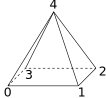
\includegraphics{tbl-5-1-4-v}
         & 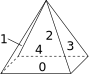
\includegraphics{tbl-5-1-4-f}
             & 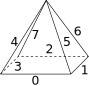
\includegraphics{tbl-5-1-4-e} \\
 四面体 & \OFkeyword{tet}
     & 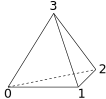
\includegraphics{tbl-5-1-5-v}
         & 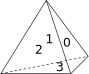
\includegraphics{tbl-5-1-5-f}
             & 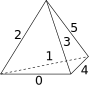
\includegraphics{tbl-5-1-5-e} \\
 くさび状四面体 & \OFkeyword{tetWedge}
     & 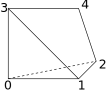
\includegraphics{tbl-5-1-6-v}
         & 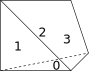
\includegraphics{tbl-5-1-6-f}
             & 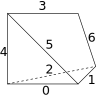
\includegraphics{tbl-5-1-6-e} \\
 \hline
\end{tabular}

 \caption{\OFtool{cellShapes}における頂点,面,辺の番号付け}
 \label{tbl:5.1}
\end{table}


\subsection{1次元や2次元,軸対称問題}
\label{ssec:5.1.4}
\index{1じげん@1次元!メッシュ}%
\index{メッシュ!1じげん@1次元}%
\index{2じげん@2次元!メッシュ}%
\index{メッシュ!2じげん@2次元}%
\index{1D!メッシュ}%
\index{メッシュ!1D}%
\index{2D!メッシュ}%
\index{メッシュ!2D}%
OpenFOAMは3次元の空間用に設計されており,
全てのメッシュもそのように定義します.
しかしながら,OpenFOAMでは,1次元や2次元
そして%
\index{じくたいしょう@軸対称!メッシュ}%
\index{メッシュ!じくたいしょう@軸対称}%
軸対称問題も解くことができ,
それには,法線方向が意図する方向であるパッチに対して,
特殊な境界条件を適用します.
具体的には,1次元や2次元問題では
\index{empty@\OFboundary{empty}!きょうかいじょうけん@境界条件}%
\index{きょうかいじょうけん@境界条件!empty@\OFboundary{empty}}%
\OFboundary{empty}のパッチタイプを使い,
軸対称問題では
\index{wedge@\OFboundary{wedge}!きょうかいじょうけん@境界条件}%
\index{きょうかいじょうけん@境界条件!wedge@\OFboundary{wedge}}%
\OFboundary{wedge}タイプを使います.
両者の使用法については\autoref{ssec:5.2.2}で触れ,
軸対称問題用の\OFkeyword{wedge}幾何形状の生成法については
\autoref{ssec:5.3.3}において述べます.



\section{境界}
\label{sec:5.2}
\index{きょうかい@境界}%
本節では境界について述べます.
境界はやや複雑です.なぜなら,形状の構成によって規定される
単純なものではなく,境界条件や境界間の接続を通して
解法を規定する不可欠の部分であるためです.
境界はメッシュ,物理量,離散化,計算法といった
多くの要素に関連しており,便宜上この章で扱います.

まず考えるべきことは,境界条件の適用のために,
境界はバラバラにされてパッチの組み合わせになるということです.
一つのパッチは一つ以上の境界面に閉じられた領域をもち,
それらが物理的に接続している必要はありません.

下に階層を示すように,パッチに関する性質は3種類あり,
\autoref{fig:5.2}では各レベルにおけるさまざまな
パッチの名前を挙げています.
下で示す階層はOpenFOAMライブラリの階層構造と類似しています.
\begin{description}
 \item[Base type(基底型)]
            形状や情報の伝達を規定
 \item[Primitive type (基本型)]
            物理量の境界条件を規定
 \item[Derived type(派生型)]
            Primitive typeから派生した,複雑な境界条件を規定
\end{description}
\OFrevision{【要検討】baseとprimitiveの訳しかた}


\begin{figure}[ht]
 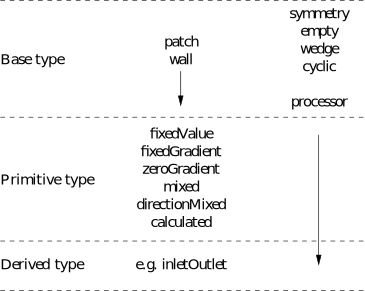
\includegraphics{fig-5-2}
 \caption{境界タイプの階層}
 \label{fig:5.2}
\end{figure}


\subsection{パッチの形式の類型化}
\label{ssec:5.2.1}
パッチの種類はメッシュと物理量のファイルに規定されます.
もう少し正確にいえば,
\begin{itemize}
 \item 基底型は\OFpath{constant/polyMesh}ディレクトリにある
       \OFpath{boundary}ファイル内の各パッチに対応する
\index{type@\OFkeyword{type}!キーワード}%
\index{キーワード!type@\OFkeyword{type}}%
       \OFkeyword{type}キーワードに従って記述されます.
 \item 数値パッチ型は,基本型または派生型となり,
       フィールドファイルの各パッチに対応する
\index{type@\OFkeyword{type}!キーワード}%
\index{キーワード!type@\OFkeyword{type}}%
       \OFkeyword{type}キーワードに従って記述されます.
\end{itemize}
例として\OFtool{sonicFoam}のケースにおける\OFpath{boundary}ファイルと
\OFpath{p}ファイル(圧力物理量ファイル)を示します.
\begin{OFverbatim}[file, linenum=17]

6
(
    inlet
    {
        type            patch;
        nFaces          50;
        startFace       10325;
    }
    outlet
    {
        type            patch;
        nFaces          40;
        startFace       10375;
    }
    bottom
    {
        type            symmetryPlane;
        nFaces          25;
        startFace       10415;
    }
    top
    {
        type            symmetryPlane;
        nFaces          125;
        startFace       10440;
    }
    obstacle
    {
        type            patch;
        nFaces          110;
        startFace       10565;
    }
    defaultFaces
    {
        type            empty;
        nFaces          10500;
        startFace       10675;
    }
)

// ************************************************************************* //
\end{OFverbatim}
\begin{OFverbatim}[file, linenum=17]
dimensions      [1 -1 -2 0 0 0 0];

internalField   uniform 1;

boundaryField
{
    inlet
    {
        type            fixedValue;
        value           uniform 1;
    }

    outlet
    {
        type            waveTransmissive;
        field           p;
        phi             phi;
        rho             rho;
        psi             psi;
        gamma           1.4;
        fieldInf        1;
        lInf            3;
        value           uniform 1;
    }

    bottom
    {
        type            symmetryPlane;
    }

    top
    {
        type            symmetryPlane;
    }

    obstacle
    {
        type            zeroGradient;
    }

    defaultFaces
    {
        type            empty;
    }
}

// ************************************************************************* //
\end{OFverbatim}
\OFpath{boundary}ファイルにおける\OFkeyword{type}には,
\OFkeyword{symmetryPlane}や\OFkeyword{empty}といった
形態的制約を受けるパッチを除くすべてのパッチに対し
\OFkeyword{patch}と記述されています.
\OFpath{p}ファイルには\OFkeyword{inlet}や
\OFkeyword{bottom}といった面に適用される基本型と
\OFkeyword{outlet}に適用される複雑な派生型が記述されています.
二つのファイルを比較すると,単純な\OFkeyword{patch}ではなく,
\OFkeyword{symmetryPlane}や\OFkeyword{empty}である場合,
基底型及び数値型で一致していることがわかります.


\subsection{ 基底型}
\label{ssec:5.2.2}
以下に基底型の種類を挙げます.
これらを規定するキーワードは\autoref{tbl:5.2}にまとめてあります.


\begin{figure}[ht]
 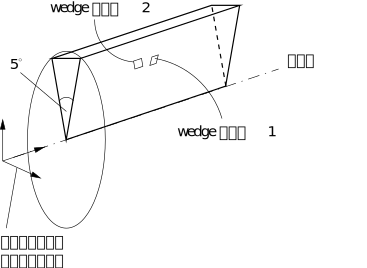
\includegraphics{fig-5-3}
 \caption{\OFkeyword{wedge}パッチを利用した軸対象形状}
 \label{fig:5.3}
\end{figure}


\begin{table}[ht]
 %#! platex UserGuideJa
\begin{tabular}{ll}
 種類 & 意味 \\
 \hline
\index{patch@\OFkeyword{patch}!キーワードエントリ}%
\index{キーワードエントリ!patch@\OFkeyword{patch}}%
 \OFkeyword{patch} & 一般的なパッチ \\
\index{symmetryPlane@\OFkeyword{symmetryPlane}!キーワードエントリ}%
\index{キーワードエントリ!symmetryPlane@\OFkeyword{symmetryPlane}}%
 \OFkeyword{symmetryPlane} & 対称面 \\
\index{empty@\OFkeyword{empty}!キーワードエントリ}%
\index{キーワードエントリ!empty@\OFkeyword{empty}}%
 \OFkeyword{empty} & 2次元形状の前後の面 \\
\index{wedge@\OFkeyword{wedge}!キーワードエントリ}%
\index{キーワードエントリ!wedge@\OFkeyword{wedge}}%
 \OFkeyword{wedge} & くさび型の前後 \\
\index{cyclic@\OFkeyword{cyclic}!キーワードエントリ}%
\index{キーワードエントリ!cyclic@\OFkeyword{cyclic}}%
 \OFkeyword{cyclic} & 周期境界面 \\
\index{wall@\OFkeyword{wall}!キーワードエントリ}%
\index{キーワードエントリ!wall@\OFkeyword{wall}}%
 \OFkeyword{wall} & 壁面(乱流の壁関数に使用) \\
\index{processor@\OFkeyword{processor}!キーワードエントリ}%
\index{キーワードエントリ!processor@\OFkeyword{processor}}%
 \OFkeyword{processor} & 並列計算時のプロセッサ間の境界 \\
 \hline
\end{tabular}

 \caption{基底型の境界の種類}
 \label{tbl:5.2}
\end{table}


\begin{figure}[ht]
 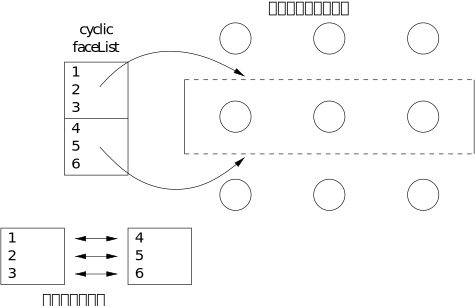
\includegraphics{fig-5-4}
 \caption{\OFkeyword{cyclic}パッチを利用した周期境界の連続形状}
 \label{fig:5.4}
\end{figure}


\begin{description}
 \item[\OFboundary{patch}]
\index{patch@\OFboundary{patch}!きょうかいじょうけん@境界条件}%
\index{きょうかいじょうけん@境界条件!patch@\OFboundary{patch}}%
            メッシュに対する形状的,
            位相的情報をなにももたないパッチ条件のための
            基礎的なパッチ (\OFkeyword{wall}の場合を除く).
            流入口や流出口など.
 \item[\OFboundary{wall}]
\index{wall@\OFboundary{wall}!きょうかいじょうけん@境界条件}%
\index{きょうかいじょうけん@境界条件!wall@\OFboundary{wall}}%
            特に専門家が壁の境界を規定するときに,
            壁に適合するパッチが以下のように
            特定可能である必要がある場合があります.
            良い例としては,壁が\OFkeyword{wall}パッチの型で
            特定されなければならない壁乱流モデルがあり,
            壁に隣接するセルの中心からの距離がパッチの一部として格納されます.
 \item[\OFboundary{symmetryPlane}]
\index{symmetryPlane@\OFboundary{symmetryPlane}!きょうかいじょうけん@境界条件}%
\index{きょうかいじょうけん@境界条件!symmetryPlane@\OFboundary{symmetryPlane}}%
            対称面
 \item[\OFboundary{empty}]
\index{empty@\OFboundary{empty}!きょうかいじょうけん@境界条件}%
\index{きょうかいじょうけん@境界条件!empty@\OFboundary{empty}}%
            OpenFOAMが常に3次元で形状を生成する一方で,
            2次元(1次元)を解くことも可能です.
            そのためには,解が必要とされない3番目(2番目)の次元に
            法線が向いている各パッチに特別な\OFkeyword{empty}条件を当てはめます.
 \item[\OFboundary{wedge}]
\index{wedge@\OFboundary{wedge}!きょうかいじょうけん@境界条件}%
\index{きょうかいじょうけん@境界条件!wedge@\OFboundary{wedge}}%
            シリンダのような2次元の%
\index{じくたいしょう@軸対称!もんだい@問題}%
            軸対称問題では,
            \autoref{fig:5.3}で示すように,
            小さい角度 (例えば$< 5\unit*{\degree}$) のくさびで,
            座標面の一つにまたがる対称面に沿って伸びている
            一つのセルとして形状が記述されます.
            軸対称くさび面は\OFkeyword{wedge}型という独自のパッチである必要があります.
            \OFtool{blockMesh}を使ったくさびの形状の生成に関する詳細は
            \autoref{ssec:5.3.3}に述べられています.
 \item[\OFboundary{cyclic}]
\index{cyclic@\OFboundary{cyclic}!きょうかいじょうけん@境界条件}%
\index{きょうかいじょうけん@境界条件!cyclic@\OFboundary{cyclic}}%
            熱交換管のような繰り返しの多い形状では,
            二つのパッチをあたかも一つのように扱うことができるようにする場合があります.
            単一の\OFkeyword{cyclic}パッチは,
            \OFkeyword{faceList}において面を二つに分割します.
            そして\autoref{fig:5.4}に示すように,
            二つの面のセットを結び付けます.
            面の各組は同じ領域のものである必要がありますが,
            同じ方向のものである必要はありません.
 \item[\OFboundary{processor}]
\index{processor@\OFboundary{processor}!きょうかいじょうけん@境界条件}%
\index{きょうかいじょうけん@境界条件!processor@\OFboundary{processor}}%
            数多くの処理の中で,計算が平行して行われている場合は,
            だいたい同じ数の格子を各処理が計算するために,
            メッシュは分けられる必要があります.
            メッシュの中の異なる部分間の境界は\OFkeyword{processor}境界とよばれます.
\end{description}


\subsection{基本型}
\label{ssec:5.2.3}
\autoref{tbl:5.3}に基本型の種類を挙げます.


\begin{table}[ht]
 %#! platex UserGuideJa
\begin{tabularx}{\textwidth}{lXp{8zw}}
 種類 & 物理量$\phi$に対して与える条件 & Data to specify \\
 \hline
\index{fixedValue@\OFboundary{fixedValue}!きょうかいじょうけん@境界条件}%
\index{きょうかいじょうけん@境界条件!fixedValue@\OFboundary{fixedValue}}%
 \OFboundary{fixedValue} & $\phi$の値が一定 & \OFkeyword{value} \\
\index{fixedGradient@\OFboundary{fixedGradient}!きょうかいじょうけん@境界条件}%
\index{きょうかいじょうけん@境界条件!fixedGradient@\OFboundary{fixedGradient}}%
 \OFboundary{fixedGradient} & $\phi$の勾配が一定 & \OFkeyword{gradient} \\
\index{zeroGradient@\OFboundary{zeroGradient}!きょうかいじょうけん@境界条件}%
\index{きょうかいじょうけん@境界条件!zeroGradient@\OFboundary{zeroGradient}}%
 \OFboundary{zeroGradient} & $\phi$の勾配が$0$ & -- \\
\index{calculated@\OFboundary{calculated}!きょうかいじょうけん@境界条件}%
\index{きょうかいじょうけん@境界条件!calculated@\OFboundary{calculated}}%
 \OFboundary{calculated} & $\phi$の境界条件が他の物理量から決まる & -- \\
\index{mixed@\OFboundary{mixed}!きょうかいじょうけん@境界条件}%
\index{きょうかいじょうけん@境界条件!mixed@\OFboundary{mixed}}%
 \OFboundary{mixed} & \OFboundary{fixedValue}と\OFboundary{fixedGradient}の組み合わせ,
     \OFkeyword{valueFraction}に依存する条件 &
         \OFkeyword{refValue},\hfil\break
\index{refGradient@\OFkeyword{refGradient}!キーワード}%
\index{キーワード!refGradient@\OFkeyword{refGradient}}%
         \OFkeyword{refGradient},\hfil\break
\index{valueFraction@\OFkeyword{valueFraction}!キーワード}%
\index{キーワード!valueFraction@\OFkeyword{valueFraction}}%
         \OFkeyword{valueFraction},\hfil\break
\index{value@\OFkeyword{value}!キーワード}%
\index{キーワード!value@\OFkeyword{value}}%
         \OFkeyword{value} \\
\index{directionMixed@\OFboundary{directionMixed}!きょうかいじょうけん@境界条件}%
\index{きょうかいじょうけん@境界条件!directionMixed@\OFboundary{directionMixed}}%
 \OFboundary{directionMixed} & パッチの法線方向に対して\OFkeyword{mixed},
     接線方向に対して\OFkeyword{fixedGradient} & \OFkeyword{refValue},\hfil\break
         \OFkeyword{refGradient},\hfil\break
         \OFkeyword{valueFraction},\hfil\break
         \OFkeyword{value} \\
 \hline
\end{tabularx}

 \caption{基本型のパッチの種類}
 \label{tbl:5.3}
\end{table}


\subsection{派生型}
\label{ssec:5.2.4}
OpenFOAMには多数の派生型境界条件があり,ここには掲載しきれません.
かわりに,ごく一部を\autoref{tbl:5.4}に紹介します.
利用できる全てのモデルの一覧を得たければ,
OpenFOAMのソースコードを参照してください.
派生型境界条件のソースコードは以下のような場所に見つかります.
\begin{itemize}
 \item \OFpath{\$FOAM SRC/finiteVolume/fields/fvPatchFields/derived}の中
 \item 特定のモデルライブラリの中.
       これはターミナルで以下のようなコマンドを実行することで探せます.
\begin{OFverbatim}{terminal}
find $FOAM_SRC -name "*derivedFvPatch*"
\end{OFverbatim}%$
 \item 特定のソルバの中.
       これはターミナルで以下のようなコマンドを実行することで探せます.
\begin{OFverbatim}{terminal}
find $FOAM_SOLVERS -name "*fvPatch*"
\end{OFverbatim}%$
\end{itemize}



\begin{table}[p]
 \rotatebox{90}{%
 \small
 \begin{minipage}{\textheight}
  %#! platex UserGuideJa
\begin{tabularx}{\textheight}{lXp{9zw}}
 \OFboundary{fixedValue}から派生 & 意味 & 指定するデータ \\
 \hline
\index{movingWallVelocity@\string\OFboundary{movingWallVelocity}!きょうかいじょうけん@境界条件}%
\index{きょうかいじょうけん@境界条件!movingWallVelocity@\string\OFboundary{movingWallVelocity}}%
 \OFboundary{movingWallVelocity} &
     ノーマルパッチの値を置き換えるのでパッチのフラックスは$0$ & \OFkeyword{value} \\
\index{pressureInletVelocity@\string\OFboundary{pressureInletVelocity}!きょうかいじょうけん@境界条件}%
\index{きょうかいじょうけん@境界条件!pressureInletVelocity@\string\OFboundary{pressureInletVelocity}}%
 \OFboundary{pressureInletVelocity} &
     流入口の$p$が分かっているとき,$\bm{U}$は,フラックスから評価され,
     パッチはノーマル. & \OFkeyword{value} \\
\index{pressureDirectedInletVelocity@\string\OFboundary{pressureDirectedInletVelocity}!きょうかいじょうけん@境界条件}%
\index{きょうかいじょうけん@境界条件!pressureDirectedInletVelocity@\string\OFboundary{pressureDirectedInletVelocity}}%
 \OFboundary{pressureDirectedInletVelocity} &
     流入口の$p$が分かっているとき,$\bm{U}$は,
     \OFkeyword{inletDirection}のフラックスから計算される. &
         \OFkeyword{value},\OFkeyword{inletDirection} \\
\index{surfaceNormalFixedValue@\string\OFboundary{surfaceNormalFixedValue}!きょうかいじょうけん@境界条件}%
\index{きょうかいじょうけん@境界条件!surfaceNormalFixedValue@\string\OFboundary{surfaceNormalFixedValue}}%
 \OFboundary{surfaceNormalFixedValue} &
     大きさによって,ベクトル境界条件をノーマルパッチに指定します.
     ベクトルの+veはドメインを指す. & \OFkeyword{value} \\
\index{totalPressure@\string\OFboundary{totalPressure}!きょうかいじょうけん@境界条件}%
\index{きょうかいじょうけん@境界条件!totalPressure@\string\OFboundary{totalPressure}}%
 \OFboundary{totalPressure} &
     全圧$p_{0} = p + \frac{1}{2}\rho|\bm{U}|^{2}$は固定.
     $\bm{U}$が変わるとそれに従い$p$も調整される. & \OFkeyword{p0} \\
\index{turbulentInlet@\string\OFboundary{turbulentInlet}!きょうかいじょうけん@境界条件}%
\index{きょうかいじょうけん@境界条件!turbulentInlet@\string\OFboundary{turbulentInlet}}%
 \OFboundary{turbulentInlet} &
     平均値のスケールに基づく変動変数について計算する &
         \OFkeyword{referenceField}, \OFkeyword{fluctuationScale} \\
 \\
 \OFboundary{fixedGradient}/\OFboundary{zeroGradient}から派生 \\
 \hline
\index{fluxCorrectedVelocity@\string\OFboundary{fluxCorrectedVelocity}!きょうかいじょうけん@境界条件}%
\index{きょうかいじょうけん@境界条件!fluxCorrectedVelocity@\string\OFboundary{fluxCorrectedVelocity}}%
 \OFboundary{fluxCorrectedVelocity} &
     フラックスから流入口の$\bm{U}$の法線成分を計算する &
         \OFkeyword{value} \\
\index{buoyantPressure@\string\OFboundary{buoyantPressure}!きょうかいじょうけん@境界条件}%
\index{きょうかいじょうけん@境界条件!buoyantPressure@\string\OFboundary{buoyantPressure}}%
 \OFboundary{buoyantPressure} &
     気圧勾配に基づく\OFboundary{fixedGradient}圧を設定する & --- \\
 \\
 \OFboundary{mixed}から派生 \\
 \hline
\index{inletOutlet@\string\OFboundary{inletOutlet}!きょうかいじょうけん@境界条件}%
\index{きょうかいじょうけん@境界条件!inletOutlet@\string\OFboundary{inletOutlet}}%
 \OFboundary{inletOutlet} &
     $\bm{U}$の向きによって\OFboundary{fixedValue}と
     \OFboundary{zeroGradient}の間で$\bm{U}$と$p$を切り替える &
         \OFkeyword{inletValue},\OFkeyword{value} \\
\index{outletInlet@\string\OFboundary{outletInlet}!きょうかいじょうけん@境界条件}%
\index{きょうかいじょうけん@境界条件!outletInlet@\string\OFboundary{outletInlet}}%
 \OFboundary{outletInlet} &
     $\bm{U}$の向きによって\OFboundary{fixedValue}と
     \OFboundary{zeroGradient}の間で$\bm{U}$と$p$を切り替える &
         \OFkeyword{outletValue},\OFkeyword{value} \\
 \OFboundary{pressureInletOutletVelocity} &
     \OFboundary{pressureInletVelocity}と
     \OFboundary{inletOutlet}の組み合わせ & \OFkeyword{value} \\
 \OFboundary{pressureDirectedInletOutletVelocity} &
     \OFboundary{pressureDirectedInletVelocity}と\OFboundary{inletOutlet}の組み合わせ &
         \OFkeyword{value},\OFkeyword{inletDirection} \\
\index{pressureTransmissive@\string\OFboundary{pressureTransmissive}!きょうかいじょうけん@境界条件}%
\index{きょうかいじょうけん@境界条件!pressureTransmissive@\string\OFboundary{pressureTransmissive}}%
 \OFboundary{pressureTransmissive} &
     周囲の圧力$p_{\infty}$に超音速圧縮波を伝える & \OFkeyword{pInf} \\
\index{supersonicFreeStream@\string\OFboundary{supersonicFreeStream}!きょうかいじょうけん@境界条件}%
\index{きょうかいじょうけん@境界条件!supersonicFreeStream@\string\OFboundary{supersonicFreeStream}}%
 \OFboundary{supersonicFreeStream} &
     斜めの衝撃を$p_{\infty}$,$T_{\infty}$,$U_{\infty}$の環境に伝える &
         \OFkeyword{pInf},\OFkeyword{TInf},\OFkeyword{UInf} \\
 その他 \\
 \hline
\index{slip@\string\OFboundary{slip}!きょうかいじょうけん@境界条件}%
\index{きょうかいじょうけん@境界条件!slip@\string\OFboundary{slip}}%
 \OFboundary{slip} & $\phi$がスカラなら\OFboundary{zeroGradient},
     $\phi$がベクトルなら法線成分は\OFboundary{fixedValue 0}で,
     接線成分は\OFboundary{zeroGradient} & --- \\
\index{partialSlip@\string\OFboundary{partialSlip}!きょうかいじょうけん@境界条件}%
\index{きょうかいじょうけん@境界条件!partialSlip@\string\OFboundary{partialSlip}}%
 \OFboundary{partialSlip} &
     混合\OFboundary{zeroGradient}/\OFboundary{slip}条件は
     \OFkeyword{valueFraction}による.\OFboundary{slip}ならば$0$. &
         \OFkeyword{valueFraction} \\
 \hline
\end{tabularx}

  Note: $p$は圧力, $\bm{U}$は速度
  \caption{派生型の種類}
  \label{tbl:5.4}
 \end{minipage}}
\end{table}



\section{\OFtool{blockMesh}ユーティリティを使ったメッシュ生成}
\label{sec:5.3}
\index{blockMesh@\OFtool{blockMesh}!ユーティリティ}%
\index{ユーティリティ!blockMesh@\OFtool{blockMesh}}%
\index{メッシュ!せいせい@生成}%
このセクションでは,OpenFOAMとともに供給される
メッシュ生成ユーティリティの\OFtool{blockMesh}について説明します.
\OFtool{blockMesh}ユーティリティは,
\index{メッシュ!こうばいづけ@勾配付け}%
勾配付けや曲がった辺を使ったパラメトリックなメッシュを作成します.

メッシュはケースの\OFpath{constant/polyMesh}ディレクトリに位置する
\index{blockMeshDict@\OFdictionary{blockMeshDict}!ディクショナリ}%
\index{ディクショナリ!blockMeshDict@\OFdictionary{blockMeshDict}}%
\OFdictionary{blockMeshDict}というディクショナリファイルから生成します.
\OFtool{blockMesh}はこのディクショナリを読み込んでメッシュを生成し,
同じディレクトリの
\index{points@\OFdictionary{points}!ディクショナリ}%
\index{ディクショナリ!points@\OFdictionary{points}}%
\OFdictionary{points},
\index{faces@\OFdictionary{faces}!ディクショナリ}%
\index{ディクショナリ!faces@\OFdictionary{faces}}%
\OFdictionary{faces},
\index{cells@\OFdictionary{cells}!ディクショナリ}%
\index{ディクショナリ!cells@\OFdictionary{cells}}%
\OFdictionary{cells}および
\index{boundary@\OFdictionary{boundary}!ディクショナリ}%
\index{ディクショナリ!boundary@\OFdictionary{boundary}}%
\OFdictionary{boundary}ファイルに
メッシュ・データを書き出します.

\OFtool{blockMesh}がよりどころとする原則は,
一つあるいは複数の3次元の六面体のブロックに領域を分割することです.
ブロックの辺は,直線,円弧またはスプラインであるかもしれません.
メッシュは,ブロックの各方向の多くのセルとして表面上指定され,
これは\OFtool{blockMesh}がメッシュ・データを生成するのに十分な情報です.

各ブロックの幾何形状は八つの頂点,
六面体の各隅のひとつによって定義されます.
頂点はラベルを使用することで各頂点にアクセスできるように
リストに書かれています. OpenFOAMは常にC++の慣習に従って,
リストの最初の要素をラベル `0' とします.
リストに従って,各頂点に番号付けがされているブロックの例を
\autoref{fig:5.5}に示します.
頂点1と5を接続する辺は,
\OFtool{blockMesh}で曲がった辺を指定できるのを
読者に思いおこさせるために曲がっています.

\autoref{ssec:5.3.3}で説明されるように,
1組以上の頂点をお互いの上で潰すことによって
八つ未満の頂点をもつブロックを生成することが可能です.

各ブロックは,
\index{ざひょうじく@座標軸!みぎてけい@右手系}
右手系である局所座標系$(x_{1}, x_{2}, x_{3})$をもちます.
右手系の軸群は,$Oz$軸を見下ろしたとき,
$Ox$軸上の点から$Oy$軸上への円弧が時計回りとなるように定義されます.
局所座標系は以下に従ってブロックの定義で提示された
頂点の順序に従って定義されます.
\begin{itemize}
 \label{p:U-130}
 \item 軸の原点はブロックの定義における最初の入力です.
       私たちの例では頂点0です.
 \item $x_{1}$の方向は,頂点0から頂点1まで動くことによって示されます.
 \item $x_{2}$の方向は,頂点1から頂点2まで動くことによって示されます.
 \item 頂点0,1,2,3は$x_{3} = 0$の平面を定義します.
 \item 頂点4は頂点0から$x_{3}$方向に動くことによって,見つけられます.
 \item 頂点5,6,および7は,頂点1,2,および3から
       それぞれ$x_{3}$の方向に動くことで,同様に見つけられます.
\end{itemize}


\begin{figure}[ht]
 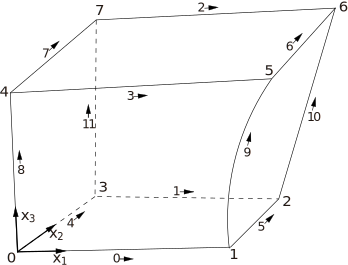
\includegraphics{fig-5-5}
 \caption{ひとつのブロック}
 \label{fig:5.5}
\end{figure}


\begin{table}[ht]
 %#! platex UserGuideJa
\begin{tabularx}{\textwidth}{lXX}
 キーワード & 説明 & 指定するデータ \\
 \hline
\index{convertToMeters@\OFkeyword{convertToMeters}!キーワード}%
\index{キーワード!convertToMeters@\OFkeyword{convertToMeters}}%
 \OFkeyword{convertToMeters} &
     頂点座標の倍率 &
         \OFkeyword{0.001}とすれば$\unit*{mm}$ \\
\index{vertices@\OFkeyword{vertices}!キーワード}%
\index{キーワード!vertices@\OFkeyword{vertices}}%
 \OFkeyword{vertices} &
     頂点座標のリスト &
         \OFkeyword{(0 0 0)} \\
\index{edges@\OFkeyword{edges}!キーワード}%
\index{キーワード!edges@\OFkeyword{edges}}%
 \OFkeyword{edges} &
\index{arc@\OFkeyword{arc}!キーワード}%
\index{キーワード!arc@\OFkeyword{arc}}%
     \OFkeyword{arc}もしくは
\index{spline@\OFkeyword{spline}!キーワード}%
\index{キーワード!spline@\OFkeyword{spline}}%
     \OFkeyword{spline}の辺を書くために使用 &
         arc 1 4 (0.939 0.342 -0.5) \\
\index{block@\OFkeyword{block}!キーワード}%
\index{キーワード!block@\OFkeyword{block}}%
 \OFkeyword{block} &
     頂点ラベルとメッシュサイズの順序リスト &
         \OFkeyword{hex (0 1 2 3 4 5 6 7)}\par
         \OFkeyword{(10 10 1)}\par
         \mbox{\OFkeyword{simpleGrading (1.0 1.0 1.0)}} \\
\index{patches@\OFkeyword{patches}!キーワード}%
\index{キーワード!patches@\OFkeyword{patches}}%
 \OFkeyword{patches} &
     パッチのリスト &
         \OFkeyword{symmetryPlane base}\par
         \OFkeyword{( (0 1 2 3) )} \\
\index{mergePatchPairs@\OFkeyword{mergePatchPairs}!キーワード}%
\index{キーワード!mergePatchPairs@\OFkeyword{mergePatchPairs}}%
 \OFkeyword{mergePatchPairs} &
     マージするパッチのリスト &
         \autoref{ssec:5.3.2}参照 \\
 \hline
\end{tabularx}

 \caption{\OFdictionary{blockMeshDict}に使用するキーワード}
 \label{tbl:5.5}
\end{table}


\subsection{\OFdictionary{blockMeshDict}ファイルの記述}
\label{ssec:5.3.1}
\OFdictionary{blockMeshDict}ファイルは,
\autoref{tbl:5.5}で説明されている
キーワードを使用するディクショナリです.
\index{convertToMeters@\OFkeyword{convertToMeters}!キーワード}%
\index{キーワード!convertToMeters@\OFkeyword{convertToMeters}}%
\OFkeyword{convertToMeters}キーワードは,
メッシュ記述におけるすべての頂点の座標にかけられる
尺度因子を指定します.例えば,
\begin{OFverbatim}[file]
convertToMeters 0.001;
\end{OFverbatim}
は,すべての座標に$0.001$をかけることを意味します.
すなわち,\OFdictionary{blockMeshDict}ファイルで引用された値が$\unit*{mm}$になります.

\subsubsection{頂点}
\label{sssec:5.3.1.1}
メッシュのブロックの頂点は,
\OFkeyword{vertices}と名づけられた
標準のリストとして以下のように与えられます.
例えば\autoref{fig:5.5}での私たちの例のブロックに関しては,
頂点は以下のとおりです.
\begin{OFverbatim}[file]
vertices
(
    ( 0 0 0 ) // vertex number 0
    ( 1 0 0.1) // vertex number 1
    ( 1.1 1 0.1) // vertex number 2
    ( 0 1 0.1) // vertex number 3
    (-0.1 -0.1 1 ) // vertex number 4
    ( 1.3 0 1.2) // vertex number 5
    ( 1.4 1.1 1.3) // vertex number 6
    ( 0 1 1.1) // vertex number 7
);
\end{OFverbatim}

\subsubsection{辺}
\label{sssec:5.3.1.2}
2頂点をつなぐ辺のそれぞれは,
デフォルトでまっすぐであると仮定されています.
しかしながら,どんな辺も,
\OFkeyword{edges}と名づけられるリストにおける入力で
曲がるように指定されるかもしれません.
そのリストはオプションです.
幾何形状がどんな曲がった辺も含んでいないなら,
それは省略されるかもしれません.

曲がった辺のための各入力は,
\autoref{tbl:5.6}に挙げられているものから
カーブのタイプを指定するキーワードとともに始まります.


\begin{table}[ht]
 %#! platex UserGuideJa
\begin{tabular}{lll}
 キーワード選択 & 説明 & 追加するエントリ \\
 \hline
\index{arc@\OFkeyword{arc}!キーワードエントリ}%
\index{キーワードエントリ!arc@\OFkeyword{arc}}%
 \OFkeyword{arc} & 円弧 & 円弧上の1点 \\
\index{simpleSpline@\OFkeyword{simpleSpline}!キーワードエントリ}%
\index{キーワードエントリ!simpleSpline@\OFkeyword{simpleSpline}}%
 \OFkeyword{simpleSpline} & スプライン曲線 & 補間点リスト \\
\index{polyLine@\OFkeyword{polyLine}!キーワードエントリ}%
\index{キーワードエントリ!polyLine@\OFkeyword{polyLine}}%
 \OFkeyword{polyLine} & 線群 & 補間点リスト \\
\index{polySpline@\OFkeyword{polySpline}!キーワードエントリ}%
\index{キーワードエントリ!polySpline@\OFkeyword{polySpline}}%
 \OFkeyword{polySpline} & スプライン群 & 補間点リスト \\
\index{line@\OFkeyword{line}!キーワードエントリ}%
\index{キーワードエントリ!line@\OFkeyword{line}}%
 \OFkeyword{line} & 直線 & --- \\
 \hline
\end{tabular}

 \caption{\OFdictionary{blockMeshDict}ディクショナリで使用可能なエッジタイプ}
 \label{tbl:5.6}
\end{table}


そして,キーワードの後には辺が接続する二つの頂点のラベルが続きます.
それに続いて,辺が通り過ぎる内挿点を指定しなければなりません.
\OFkeyword{arc}には,円弧が横切ることになる一つの内挿点が必要です.
\OFkeyword{simpleSpline},\OFkeyword{polyLine},
および\OFkeyword{polySpline}に関しては,内挿点のリストが必要です.
\OFkeyword{line}辺は,デフォルトとして実行されるオプションと
全く同等であり,内挿点を全く必要としません.
\OFkeyword{line}辺を使用する必要は全くありませんが,
それが完全性のために含まれていることに注意してください.
\autoref{fig:5.6}での私たちの例のブロックでは,
内挿点$(1.1, 0.0, 0.5)$を通して以下のように
頂点1と5をつなぐ\OFkeyword{arc}辺を指定します.
\begin{OFverbatim}[file]
edges
(
    arc 1 5 (1.1 0.0 0.5)
);
\end{OFverbatim}

\subsubsection{ブロック}
\label{sssec:5.3.1.3}
ブロックの定義は
\index{blocks@\OFkeyword{blocks}!キーワード}%
\index{キーワード!blocks@\OFkeyword{blocks}}%
\OFkeyword{blocks}と名づけられたリストに含まれています.
各ブロックの定義は,セクション\autoref{sec:5.3}で示された順序をもつ
頂点ラベルのリストからなる複合入力です.
ベクトルが各方向に必要なセルの数,タイプ,
および各方向のセル拡大比のリストを与えます.

そして,ブロックは以下のとおり定義されます.
\begin{OFverbatim}[file]
blocks
(
    hex (0 1 2 3 4 5 6 7) // vertex numbers
    (10 10 10) // numbers of cells in each direction
    simpleGrading (1 2 3) // cell expansion ratios
);
\end{OFverbatim}
それぞれのブロックの定義は以下のとおりです.
\begin{description}
 \item[Vertex numbering]
\index{blockMesh@\OFtool{blockMesh}!じっこうかのう@実行可能な頂点の番号付け}%
            \OFpath{OpenFOAM-1.7.1/cellModels}ファイルに
            定義されているように,最初の入力がブロックの
\index{けいじょう@形状}%
            形状識別子です.
            いつもブロックが六面体であるので,
            いつも形は\OFkeyword{hex}です.
            \pageref{p:U-130}ページで説明された方法で並べられた
            頂点番号のリストが従います.
 \item[Number of cells]
            2番目の入力はそのブロックの$x_{1}$,$x_{2}$,$x_{3}$と
            それぞれの方向のセルの数を与えます.
 \item[Cell expansion ratios]
\index{ブロック!かくだいりつ@拡大率}%
\index{セル!かくだいりつ@拡大率}%
            3番目の入力はブロックにおける各方向へのセルの拡大比を与えます.
            拡大比は,メッシュが指定された方向に段階的なものにするか,
            または精製されるのを可能にします.
            比率$\delta_{\mathrm{e}}$は\autoref{fig:5.6}に示すように,
            ブロックのひとつの辺に沿った終わりのセルの幅の,
            辺に沿った始めのセル幅$\delta_{\mathrm{s}}$への比です.
            以下のキーワードのそれぞれは\OFtool{blockMesh}で利用可能な
\index{メッシュ!こうばいづけ@勾配付け}%
            勾配付けの仕様の二つのタイプの一つを指定します.
            \begin{description}
             \item[simpleGrading]
\index{simpleGrading@\OFkeyword{simpleGrading}!キーワード}%
\index{キーワード!simpleGrading@\OFkeyword{simpleGrading}}%
                        簡単な記述で,局所的な$x_{1}$,$x_{2}$と$x_{3}$方向それぞれに一様な
                        拡大比を,三つの拡大比だけで指定します.例えば
\begin{OFverbatim}[file]
simpleGrading (1 2 3)
\end{OFverbatim}
             \item[edgeGrading]
\index{edgeGrading@\OFkeyword{edgeGrading}!キーワード}%
\index{キーワード!edgeGrading@\OFkeyword{edgeGrading}}%
                        完全なセルの拡大比の記述は,
                        \autoref{fig:5.5}に矢印で
                        「最初のセルから最後のセル」の方向を表した
                        スキームに従って番号付けられた
                        ブロックの各辺に比率を与えます.
                        例えば,このようなものです.
\begin{OFverbatim}[file]
edgeGrading (1 1 1 1 2 2 2 2 3 3 3 3)
\end{OFverbatim}
                        これは,辺$0$--$3$に沿ったセル幅の比率が$1$,
                        辺$4$--$7$に沿った比率が$2$であり,
                        辺$8$--$11$に沿った比率が$3$である
                        ということであることを意味しており,
                        上述した\OFkeyword{simpleGrading}の例に
                        まったく同等です.
            \end{description}
\end{description}


\begin{figure}[ht]
 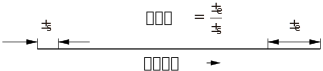
\includegraphics{fig-5-6}
 \caption{ブロックの辺に沿って段階わけされたメッシュ}
 \label{fig:5.6}
\end{figure}


\subsubsection{パッチ}
\label{sssec:5.3.1.4}
\index{patches@\OFkeyword{patches}!キーワード}%
\index{キーワード!patches@\OFkeyword{patches}}%
\OFkeyword{patches}というリストで
メッシュのパッチを与えます.
リストにおける各パッチは以下を含む複合記入です.
\begin{itemize}
 \item パッチタイプ,いくつかの境界条件が適用されている一般的なパッチか,
       \autoref{tbl:5.1}にリストアップされていて
       セクション\autoref{ssec:5.2.2}で説明される特定の幾何的条件のどちらか.
 \item パッチを作るブロックの面のリスト,
       便利にパッチを特定できる名前が推奨されるものの,
       名前はユーザの選択に任されます.
       例えば\OFkeyword{quoteTextinlet},
       この名前は,境界条件をフィールドデータファイルに
       設定するための識別子として使用されます.
       \OFtool{blockMesh}は\OFkeyword{patches}リストから省かれる
       どんな境界パッチからも面を集め,
       それらに\OFkeyword{defaultFaces}とよばれる
       \OFkeyword{empty}タイプからなるデフォルトパッチを割り当てます.
       これは,2次元の幾何形状において,
       それらが必要に応じて\OFkeyword{empty}パッチに
       集められるのを知りながら,
       ユーザは2次元平面にあるブロック面を
       省略する選択ができることを意味します.
\end{itemize}
\autoref{fig:5.5}での例のブロックに戻って,
もし左面に流入があり,右面における流出があり,
他の四つの表面が壁であるならば,以下のとおりパッチは定義できるでしょう.
\begin{OFverbatim}[file]
patches // keyword
(
    patch // patch type for patch 0
    inlet // patch name
    (
        (0 4 7 3) // block face in this patch
    ) // end of 0th patch definition
    patch // patch type for patch 1
    outlet // arbitrary patch name
    (
        (1 2 6 5)
    )
    wall
    walls
    (
        (0 1 5 4)
        (0 3 2 1)
        (3 7 6 2)
        (4 5 6 7)
    )
);
\end{OFverbatim}
それぞれのブロック面は四つの頂点番号のリストによって定義されます.
頂点が与えられる順序は,ブロックの中から見て,
どの頂点からも始めても,他の頂点を定義するために
時計回りに面を回るようなものにならなければなりません.


\subsection{複数のブロック}
\label{ssec:5.3.2}
1ブロック以上を使用することでメッシュを作成できます.
そのような事情では,メッシュは前述のテキストで
説明されるように作成されます.
唯一の追加設定がブロック間の接続です.
そこに,二つの異なる可能性があります.
\begin{description}
 \item[face matching]
            あるブロックのパッチを包括する面の組が,
            別のブロックのパッチを包括する面の組と全く同じ位置にあるものです.
 \item[face merging]
            あるブロックのパッチからの面のグループは,
            二つのブロックをつなげながら新しい内部の面の組を作成するために,
            別のブロックのパッチからの面の別のグループに関連づけられます.
\end{description}
face matchingで2ブロックをつなげるためには,
接続を形成する二つのパッチが
\OFkeyword{patches}リストから単に無視されるべきです.
\OFtool{blockMesh}は,面が外部の境界を形成せず,
同じところに位置する各組を,2ブロックからのセルを接続する,
ひとつの内部面に結合するのを特定します.

もうひとつのface margingは,
併合されるブロックパッチがまず\OFkeyword{patches}リストで
定義されることを必要とします.面が併合されるパッチのそれぞれの組が,
\OFkeyword{mergePatchPairs}というオプションリストに含まなければなりません.
\OFkeyword{mergePatchPairs}の形式は以下のとおりです.
\begin{OFverbatim}[file]
mergePatchPairs
(
    ( <masterPatch> <slavePatch> ) // merge patch pair 0
    ( <masterPatch> <slavePatch> ) // merge patch pair 1
    ...
)
\end{OFverbatim}
パッチの組は,最初のパッチはマスタになり,
2番目はスレイブになると解釈されます.
併合するための規則は以下のとおりです
\begin{itemize}
 \item マスタパッチの面は元々定義されているままで,
       すべての頂点は元の位置にあります.
 \item スレイブパッチの面は,スレイブとは多少異なる
       マスタパッチに投影されます.
 \item スレイブ面のどんな頂点の位置も,
       面の最小許容値より短いあらゆる辺を除去するために,
       \OFtool{blockMesh}によって調整されるかもしれません.
 \item パッチが\autoref{fig:5.7}に示されるように重なるなら,
       併合しない各面が,境界条件を適用しなければならない,
       元のパッチの外部面として残ります.
 \item パッチのすべての面が併合されているなら,
       パッチ自体は表面を全く含まないので,除去されます.
\end{itemize}


\begin{figure}[ht]
 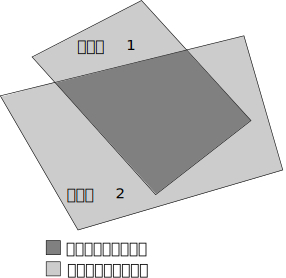
\includegraphics{fig-5-7}
 \caption{重なったパッチのマージ}
 \label{fig:5.7}
\end{figure}


結果的に,スレイブパッチのオリジナルの幾何形状が,
併合の間必ずしも,完全に保存されるというわけではないということです.
したがって,たとえば,円筒状のブロックが,
より大きいブロックにつなげられている場合では,
円筒状の形が正しく保存されるように,
マスタパッチを円筒状のブロックにするのが賢いでしょう.
併合手順を確実に成功させるためのいくつかの追加の推奨策があります.
\begin{itemize}
 \item 2次元の幾何学形状では,2次元平面の外での3次元目のセルサイズは,
       2次元平面でのセルの幅・高さと同様であるべきです.
 \item 二度パッチを併合すること,すなわち,
       \OFkeyword{mergePatchPairs}で二度それを含めるのは勧められません.
 \item 併合されるべきパッチが,他の併合されるパッチと共通の
       辺を共有するところでは,両方がマスタパッチとして宣言されるべきです.
\end{itemize}


\subsection{8頂点未満のブロックの作成}
\label{ssec:5.3.3}
八つ未満の頂点でブロックを作成するために,
1組以上の頂点をお互いの上で潰すことが可能です.
頂点を潰す最も一般的な例としては,
セクション\autoref{ssec:5.2.2}で説明した
\index{wedge@\OFboundary{wedge}!きょうかいじょうけん@境界条件}%
\index{きょうかいじょうけん@境界条件!wedge@\OFboundary{wedge}}%
\OFboundary{wedge}パッチタイプを使用する
2次元の%
\index{じくたいしょう@軸対称!もんだい@問題}%
軸対称問題のための6面のくさび型ブロックを作成するときがあります.
\autoref{fig:5.8}に示す私たちの例における,
ブロックの簡易型のバージョンを使用することで,
過程をわかりやすく例証します.
頂点7を頂点4に,頂点6を頂点5に置いて潰すことによって,
くさび型ブロックを作成したいということです.
これは,ブロック番号7を4で,6を5でそれぞれ交換することによって
簡単にできます.するとブロック番号はこのようになります.
\begin{OFverbatim}[file]
hex (0 1 2 3 4 5 5 4)
\end{OFverbatim}


\begin{figure}[ht]
 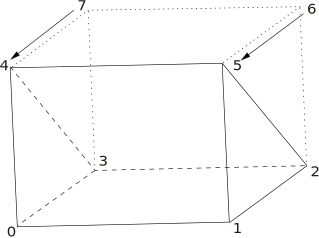
\includegraphics{fig-5-8}
 \caption{くさび形をしたブロックを六つの接点で作る}
 \label{fig:5.8}
\end{figure}


潰れている頂点を含むブロック面を考えることで,
同じことがパッチにも適用でき,以前\OFkeyword{(4 5 6 7)}だったものが,
\OFkeyword{(4 5 5 4)}になります.これは面積をもたないブロック面で,
\OFkeyword{polyMesh}で面のないパッチを生成します.
これは\OFpath{boundary}ファイルにおいて
同様の場合でも見ることができることと同じです.
パッチは\OFdictionary{blockMeshDict}で,
\OFkeyword{empty}として指定されるべきです.
そしてどんなフィールドの境界条件も結果的に\OFkeyword{empty}であるはずです.


\subsection{\OFtool{blockMesh}の実行}
\label{ssec:5.3.4}
\autoref{sec:3.3}で説明されたように,
\OFpath{<case>}ディレクトリのケースに対して
\OFtool{blockMesh}を実行するためには,
以下のようにすればコマンドラインで実行できます.
\begin{OFverbatim}[terminal]
blockMesh -case <case>
\end{OFverbatim}
\index{blockMeshDict@\OFdictionary{blockMeshDict}!ディクショナリ}%
\index{ディクショナリ!blockMeshDict@\OFdictionary{blockMeshDict}}%
\OFdictionary{blockMeshDict}ファイルは,
サブディレクトリ\OFpath{constant/polyMesh}に存在しなければなりません.



\section{\OFtool{snappyHexMesh}ユーティリティを使ったメッシュ生成}
\label{sec:5.4}
\index{snappyHexMesh@\OFtool{snappyHexMesh}!ユーティリティ}%
\index{ユーティリティ!snappyHexMesh@\OFtool{snappyHexMesh}}%
\index{メッシュ!せいせい@生成}%
OpenFOAMのメッシュ生成ユーティリティ
\OFtool{snappyHexMesh}について解説します.
\OFtool{snappyHexMesh}は
\index{Stereolithography (STL)}%
STL形式の三角の表面形状から
六面体と
\index{メッシュ!ぶんかつろくめんたい@分割六面体}%
分割六面体の3次元メッシュを自動的に生成します.
はじめのメッシュの細分化と,後に現れる分割の六進法のメッシュの
\index{ひょうめんメッシュ@表面メッシュ}%
表面形状への変形を繰り返して表面形状に近づいていきます.
オプションとして,現れたメッシュを縮小させ,
レイヤセルを挿入することができます.
メッシュの細分化のレベルは非常に柔軟性が高く,
表面の処理はあらかじめ定義したメッシュの水準に適合します.
\OFtool{snappyHexMesh}は毎回負荷を平均化して並列動作をします.


\begin{figure}[ht]
 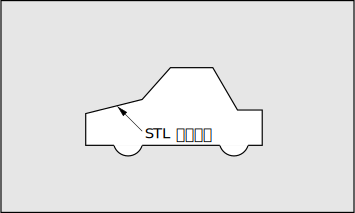
\includegraphics{fig-5-9}
 \caption{\OFtool{snappyHexMesh}における2次元メッシュ問題の概略図}
 \label{fig:5.9}
\end{figure}


\subsection{\OFtool{snappyHexMesh}によるメッシュ生成の過程}
\label{ssec:5.4.1}
\autoref{fig:5.9}に示す概略図を用いて
メッシュを\OFtool{snappyHexMesh}によって生成する流れを説明します.
\index{メッシュ!Stereolithography (STL)}%
Stereolithography (STL) 形式の
\index{メッシュ!ひょうめん@表面}%
表面形状で描かれた対象を囲む長方形の部分
(図中のグレーの部分)にメッシュを作成することを目的とします.
これは外部の空気力学のシミュレーションにおいて典型的な手法です.
あくまでも\OFtool{snappyHexMesh}は3次元メッシュの生成ツールですが,
簡単のためここでは2次元の図を使用しています.

\OFtool{snappyHexMesh}を実行するには以下の準備が必要です.
\begin{itemize}
 \item 2進法またはASCIIで表されたSTL形式による表面形状データを
       ケースディレクトリの\OFpath{triSurface}サブディレクトリに置く.
 \item \autoref{ssec:5.4.2}で述べる\OFtool{blockMesh}を使用して,
       解析領域の範囲とメッシュ密度の基準を決めるために
       六角形の基礎メッシュを作成しておく.
 \item ケースの\OFpath{system}ディレクトリにある
\index{snappyHexMeshDict@\OFpath{snappyHexMeshDict}!ファイル}%
\index{ファイル!snappyHexMeshDict@\OFpath{snappyHexMeshDict}}%
       \OFpath{snappyHexMeshDict}ディクショナリに,適切な内容を入力する.
\end{itemize}
\OFpath{snappyHexMeshDict}ディクショナリには,
\index{snappyHexMesh@\OFtool{snappyHexMesh}!ユーティリティ!メッシュせいせいプロセス@メッシュ生成プロセス}%
メッシュ生成の様々な段階を管理する最上位での変更や,
各過程における個々のサブディレクトリがあります.
入力例を\autoref{tbl:5.7}に示します.


\begin{table}[ht]
 %#! platex UserGuideJa
\begin{tabularx}{\textwidth}{lXl}
 キーワード & 意味 & 例 \\
 \hline
 \tblstrut
\index{castellatedMesh@\string\OFkeyword{castellatedMesh}!キーワード}%
\index{キーワード!castellatedMesh@\string\OFkeyword{castellatedMesh}}%
 \OFkeyword{castellatedMesh} & 階段状のメッシュを作成するか & \OFkeyword{true} \\
\index{snap@\string\OFkeyword{snap}!キーワード}%
\index{キーワード!snap@\string\OFkeyword{snap}}%
 \OFkeyword{snap} & 表面への適合操作をするか & \OFkeyword{true} \\
\index{doLayers@\string\OFkeyword{doLayers}!キーワード}%
\index{キーワード!doLayers@\string\OFkeyword{doLayers}}%
 \OFkeyword{doLayers} & レイヤの追加をするか & \OFkeyword{true} \\
\index{mergeTolerance@\string\OFkeyword{mergeTolerance}!キーワード}%
\index{キーワード!mergeTolerance@\string\OFkeyword{mergeTolerance}}%
 \OFkeyword{mergeTolerance} &
 マージする許容値.初期メッシュのバウンディングボックスに対する比 &
 \OFkeyword{1e-06} \\
\index{debug@\string\OFkeyword{debug}!キーワード}%
\index{キーワード!debug@\string\OFkeyword{debug}}%
 \OFkeyword{debug} & 中間メッシュと画面出力の制御 \\
 & 最終メッシュのみ出力 & \OFkeyword{0} \\
 & 中間メッシュの出力 & \OFkeyword{1} \\
 & 後処理のため\OFkeyword{cellLevel}を付けた\OFkeyword{volScalarField}を出力 & \OFkeyword{2} \\
 & \OFpath{.obj}ファイルとして中間時の交線を出力 & \OFkeyword{4} \\
\index{geometry@\string\OFkeyword{geometry}!キーワード}%
\index{キーワード!geometry@\string\OFkeyword{geometry}}%
 \OFkeyword{geometry} & 使用する全表面形状のサブディクショナリ \\
\index{castellatedMeshControls@\string\OFkeyword{castellatedMeshControls}!キーワード}%
\index{キーワード!castellatedMeshControls@\string\OFkeyword{castellatedMeshControls}}%
 \OFkeyword{castellatedMeshControls} & 階段状メッシュ制御のサブディクショナリ \\
\index{snapControls@\string\OFkeyword{snapControls}!キーワード}%
\index{キーワード!snapControls@\string\OFkeyword{snapControls}}%
 \OFkeyword{snapControls} & 表面スナップ制御のサブディクショナリ \\
\index{addLayersControls@\string\OFkeyword{addLayersControls}!キーワード}%
\index{キーワード!addLayersControls@\string\OFkeyword{addLayersControls}}%
 \OFkeyword{addLayersControls} & レイヤ追加制御のサブディクショナリ \\
\index{meshQualityControls@\string\OFkeyword{meshQualityControls}!キーワード}%
\index{キーワード!meshQualityControls@\string\OFkeyword{meshQualityControls}}%
 \OFkeyword{meshQualityControls} & メッシュ品質制御のサブディクショナリ \\
 \hline
\end{tabularx}

 \caption{\OFtool{snappyHexMeshDict}の最上位のキーワード}
 \label{tbl:5.7}
\end{table}


\OFtool{snappyHexMesh}で読み込む形状は
\OFpath{snappyHexMeshDict}内の\OFkeyword{geometory}の部分に記述します.
形状はSTL形状またはOpenFOAMにおける幾何実体によって指定されます.
以下に例を示します.
\begin{OFverbatim}[file]
geometry
  {
      sphere.stl // STL filename
      {
          type triSurfaceMesh;
          regions
          {
              secondSolid             // Named region in the STL file
              {
                  name mySecondPatch; // User-defined patch name
              }                       // otherwise given sphere.stl_secondSolid
          }
      }

      box1x1x1  // User defined region name
      {
          type   searchableBox;       // region defined by bounding box
          min    (1.5 1 -0.5);
          max    (3.5 2 0.5);
      }

      sphere2  // User defined region name
      {
          type   searchableSphere;    // region defined by bounding sphere
          centre (1.5 1.5 1.5);
          radius 1.03;
      }
  };
\end{OFverbatim}


\subsection{六面体基礎メッシュの作成}
\label{ssec:5.4.2}
\OFtool{snappyHexMesh}を実行する前に\OFtool{blockMesh}を使用して
\autoref{fig:5.10}が示すように,
解析領域をカバーする六面体セルの
\index{snappyHexMesh@\OFtool{snappyHexMesh}!ユーティリティ!きそメッシュ@基礎メッシュ}%
基礎メッシュを作成します.
基礎メッシュの生成時は以下の点に注意しなければなりません.
\begin{itemize}
 \item メッシュは六面体のみで構成されていること
 \item セルのアスペクト比がほぼ$1$であること.
       少なくとも連続したスナップが行われる表面近傍で
       そうでなければスナップの収束に時間がかかり,不良の原因となる.
 \item STLの表面とセルのエッジが最低でも一箇所は交差すること.
       つまり,一つのセルだけのメッシュでは機能しない.
\end{itemize}


\begin{figure}[ht]
 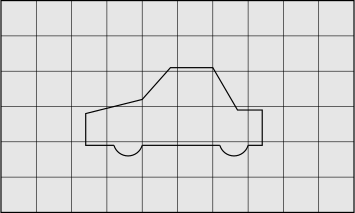
\includegraphics{fig-5-10}
 \caption{\OFtool{snappyHexMesh}実行前の基礎メッシュの生成}
 \label{fig:5.10}
\end{figure}


\subsection{面と輪郭に合わせたセルの分割}
\label{ssec:5.4.3}
\index{snappyHexMesh@\OFtool{snappyHexMesh}!ユーティリティ!セルのぶんかつ@セルの分割}%
セルの分割は,\OFpath{snappyHexMeshDict}の
\index{castellatedMeshControls@\OFsubdictionary{castellatedMeshControls}!ディクショナリ}%
\index{ディクショナリ!castellatedMeshControls@\OFsubdictionary{castellatedMeshControls}}%
\OFsubdictionary{castellatedMeshControls}サブディクショナリにおいて設定して実行します.
\OFsubdictionary{castellatedMeshControls}の入力の例を\autoref{tbl:5.8}に示します.


\begin{table}[ht]
 %#! platex UserGuideJa
\begin{tabularx}{\textwidth}{lXl}
 キーワード & 意味 & 例 \\
 \hline
\index{locationInMesh@\string\OFkeyword{locationInMesh}!キーワード}%
\index{キーワード!locationInMesh@\string\OFkeyword{locationInMesh}}%
 \OFkeyword{locationInMesh} & メッシュが作成される領域内の位置ベクトル & \OFkeyword{(5 0 0)} \\
 & ベクトルが細分化の前または最中にセルの面と一致してはいけない \\
\index{maxLocalCells@\string\OFkeyword{maxLocalCells}!キーワード}%
\index{キーワード!maxLocalCells@\string\OFkeyword{maxLocalCells}}%
 \OFkeyword{maxLocalCells} & 細分化中におけるプロセッサあたりのセルの数の最大値 & \OFkeyword{1e+06} \\
\index{maxGlobalCells@\string\OFkeyword{maxGlobalCells}!キーワード}%
\index{キーワード!maxGlobalCells@\string\OFkeyword{maxGlobalCells}}%
 \OFkeyword{maxGlobalCells} & 細分化中におけるセルの数の総数 (i.e. 除去の前) & \OFkeyword{2e+06} \\
\index{minRefinementCells@\string\OFkeyword{minRefinementCells}!キーワード}%
\index{キーワード!minRefinementCells@\string\OFkeyword{minRefinementCells}}%
 \OFkeyword{minRefinementCells} & 細分化すべきセルの数の最低値.この値以下だと停止 & \OFkeyword{0} \\
\index{nCellsBetweenLevels@\string\OFkeyword{nCellsBetweenLevels}!キーワード}%
\index{キーワード!nCellsBetweenLevels@\string\OFkeyword{nCellsBetweenLevels}}%
 \OFkeyword{nCellsBetweenLevels} & 異なる細分化レベル間のセルの緩衝レイヤーの数 & \OFkeyword{1} \\
\index{resolveFeatureAngle@\string\OFkeyword{resolveFeatureAngle}!キーワード}%
\index{キーワード!resolveFeatureAngle@\string\OFkeyword{resolveFeatureAngle}}%
 \OFkeyword{resolveFeatureAngle} & 角度がこの値を超えている交点をもつセルに最高レベルの細分化を行う & \OFkeyword{30} \\
\index{features@\string\OFkeyword{features}!キーワード}%
\index{キーワード!features@\string\OFkeyword{features}}%
 \OFkeyword{features} & 細分化に対する機能リスト \\
\index{refinementSurfaces@\string\OFkeyword{refinementSurfaces}!キーワード}%
\index{キーワード!refinementSurfaces@\string\OFkeyword{refinementSurfaces}}%
 \OFkeyword{refinementSurfaces} & 細分化に対する表面ディクショナリ \\
\index{refinementRegions@\string\OFkeyword{refinementRegions}!キーワード}%
\index{キーワード!refinementRegions@\string\OFkeyword{refinementRegions}}%
 \OFkeyword{refinementRegions} & 細分化に対する領域ディクショナリ \\
 \hline
\end{tabularx}

 \caption{\OFdictionary{snappyHexMeshDict}の
\index{castellatedMeshControls@\OFsubdictionary{castellatedMeshControls}!ディクショナリ}%
\index{ディクショナリ!castellatedMeshControls@\OFsubdictionary{castellatedMeshControls}}%
 \OFsubdictionary{castellatedMeshControls}サブディクショナリのキーワード}
 \label{tbl:5.8}
\end{table}


\autoref{fig:5.11}で示されたように,
最初に領域内で指定された輪郭に従って選択されたセルで分割が開始します.


\begin{figure}[ht]
 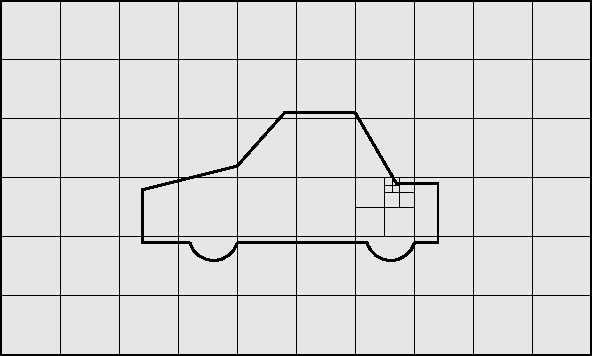
\includegraphics{fig-5-11}
 \caption{\OFtool{snappyHexMesh}の輪郭によるセルの分割}
 \label{fig:5.11}
\end{figure}


\OFkeyword{castellatedMeshControls}サブディクショナリの輪郭のリストにおいて
\OFpath{edgeMesh}ファイルの名前と細分化のレベルを記述します.
\begin{OFverbatim}[file]
features
  (
      {
          file "someLine.eMesh"; // file containing edge mesh
          level 2;               // level of refinement
      }
  );
\end{OFverbatim}

輪郭の細分化に続き,\autoref{fig:5.12}に示すように,
指定された表面における分割のためにセルが選択されます.


\begin{figure}[ht]
 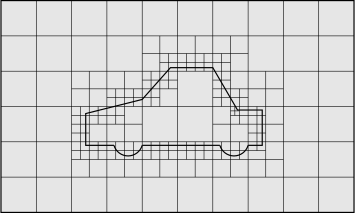
\includegraphics{fig-5-12}
 \caption{\OFtool{snappyHexMesh}の表面によるセルの分割}
 \label{fig:5.12}
\end{figure}


\OFkeyword{castellatedMeshControls}の
\OFdictionary{refinementSurface}ディクショナリで,各STL表面のディクショナリ入力と,
型の最小,最大細分化のデフォルトレベルの指定を行います.
(\verb|<min> <max>|) 最小レベルは表面のいたるところに適用され,
最大レベルは
\index{resolveFeatureAngle@\OFkeyword{resolveFeatureAngle}!キーワード}%
\index{キーワード!resolveFeatureAngle@\OFkeyword{resolveFeatureAngle}}%
\OFkeyword{resolveFeatureAngle}に規定される
角度を超過する交点をもつセルに適用されます.

細分化はSTL表面の特定領域に対して複数回行うことができます.
領域の入力は\OFsubdictionary{regions}サブディクショナリに収められています.
各領域の入力に対するキーワードは領域の名前そのものであり,
細分化のレベルはさらにサブのディクショナリに含まれます.以下の入力例を参考にしてください.
\begin{OFverbatim}[file]
refinementSurfaces
  {
      sphere.stl
      {
          level (2 2); // default (min max) refinement for whole surface
          regions
          {
              secondSolid
              {
                  level (3 3); // optional refinement for secondSolid region
              }
          }
      }
  }
\end{OFverbatim}


\subsection{セルの除去}
\label{ssec:5.4.4}
\index{snappyHexMesh@\OFtool{snappyHexMesh}!ユーティリティ!セルのじょきょ@セルの除去}%
輪郭と表面の分割が完了するとセルの除去が始まります.
セルの除去には領域内の有界表面によって完全に囲まれる
一つ以上の範囲が必要です.
セルが保持される領域は,\OFkeyword{castellatedMeshControls}の
\index{locationInMesh@\OFkeyword{locationInMesh}!キーワード}%
\index{キーワード!locationInMesh@\OFkeyword{locationInMesh}}%
\OFkeyword{locationInMesh}キーワードに指定される
領域内の位置ベクトルによって特定されます.
セルの体積のほぼ$50\unit{\%}$以上が領域内に存在する場合保持されます.
残りのセルは\autoref{fig:5.13}に示すように除去されます.


\begin{figure}[ht]
 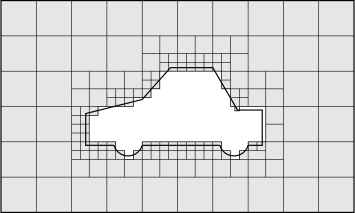
\includegraphics{fig-5-13}
 \caption{snappyHexMeshにおけるメッシュの除去}
 \label{fig:5.13}
\end{figure}


\subsection{特定領域内のセルの分割}
\label{ssec:5.4.5}
特定領域に含まれるセルはさらに細分化されます.
\autoref{fig:5.14}では長方形の濃いグレーの領域が該当します.
\index{castellatedMeshControls@\OFsubdictionary{castellatedMeshControls}!ディクショナリ}%
\index{ディクショナリ!castellatedMeshControls@\OFsubdictionary{castellatedMeshControls}}%
\OFsubdictionary{castellatedMeshControls}内の
\index{refinementRegions@\OFsubdictionary{refinementRegions}!キーワード}%
\index{キーワード!refinementRegions@\OFsubdictionary{refinementRegions}}%
\OFsubdictionary{refinementRegions}サブディクショナリでは,
\OFsubdictionary{geometry}サブディクショナリにおいて指定された
領域の細分化の入力を行います.細分化の
\index{mode@\OFkeyword{mode}!キーワード}%
\index{キーワード!mode@\OFkeyword{mode}}%
\OFkeyword{mode}と対象領域は以下のとおりです.
\begin{description}
 \item[\OFkeyword{inside}]
\index{inside@\OFkeyword{inside}!キーワードエントリ}%
\index{キーワードエントリ!inside@\OFkeyword{inside}}%
            領域の内部を細分化します.
 \item[\OFkeyword{outside}]
\index{outside@\OFkeyword{outside}!キーワードエントリ}%
\index{キーワードエントリ!outside@\OFkeyword{outside}}%
            領域の外部を細分化します.
 \item[\OFkeyword{distance}]
\index{distance@\OFkeyword{distance}!キーワードエントリ}%
\index{キーワードエントリ!distance@\OFkeyword{distance}}%
            表面からの距離にしたがって細分化します.
            レベルキーワードを用いることで複数の距離にある異なるレベルにも適用できます.
\end{description}
\index{refinementRegions@\OFkeyword{refinementRegions}!キーワード}%
\index{キーワード!refinementRegions@\OFkeyword{refinementRegions}}%
\OFkeyword{refinementRegions}では,細分化のレベルを
\index{levels@\OFkeyword{levels}!キーワード}%
\index{キーワード!levels@\OFkeyword{levels}}%
\OFkeyword{levels}入力リストによって
(\verb|<距離> <レベル>|) のように記述します.
\OFkeyword{inside}と\OFkeyword{outside}の細分化の場合,
\verb|<distance>|は不要で無視されますが,
指定する必要があります.以下に入力例を示します.
\begin{OFverbatim}[file]
refinementRegions
{
    box1x1x1
    {
        mode inside;
        levels ((1.0 4));         // refinement level 4 (1.0 entry ignored)
    }

    sphere.stl
    {                             // refinement level 5 within 1.0 m
        mode distance;            // refinement level 3 within 2.0 m
        levels ((1.0 5) (2.0 3)); // levels must be ordered nearest first
    }
}
\end{OFverbatim}


\begin{figure}[ht]
 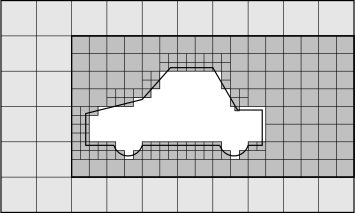
\includegraphics{fig-5-14}
 \caption{\OFtool{snappyHexMesh}の領域によるセルの分割}
 \label{fig:5.14}
\end{figure}


\subsection{面へのスナップ}
\label{ssec:5.4.6}
\index{snappyHexMesh@\OFtool{snappyHexMesh}!ユーティリティ!めんへのスナップ@面へのスナップ}%
メッシュを生成する次の段階として,
メッシュを平滑化するためにセルの頂点を表面に移動します.
その手順は以下の通りです.
\begin{enumerate}
 \item\label{enm:5.4.6-1}
      ギザギザの境界面の頂点をSTL表面上に移動する
 \item\label{enm:5.4.6-2}
      最後に移動した境界の頂点を用いて内部メッシュの緩和を求める
 \item メッシュの水準に影響をもたらす頂点を探す
 \item 最初の数値 (\ref{enm:5.4.6-1}) での頂点の移動を減らし,
       \ref{enm:5.4.6-2}からメッシュの質が
       満足できるレベルに達するまで繰り返す.
\end{enumerate}
\autoref{tbl:5.9}に示す\OFpath{snappyHexMeshDict}の
\OFsubdictionary{snapControls}サブディクショナリにおいて設定をします.


\begin{table}[ht]
 %#! platex UserGuideJa
\begin{tabularx}{\textwidth}{lXl}
 キーワード & 意味 & 例 \\
 \hline
\index{nSmoothPatch@\OFkeyword{nSmoothPatch}!キーワード}%
\index{キーワード!nSmoothPatch@\OFkeyword{nSmoothPatch}}%
 \OFkeyword{nSmoothPatch} & 表面との一致に至る前に行うパッチの平滑化の回数 & 3 \\
\index{tolerance@\OFkeyword{tolerance}!キーワード}%
\index{キーワード!tolerance@\OFkeyword{tolerance}}%
 \OFkeyword{tolerance} & 局所的な輪郭の最大長さに対する点と表面の距離の比の許容範囲 & 4.0 \\
\index{nSolveIter@\OFkeyword{nSolveIter}!キーワード}%
\index{キーワード!nSolveIter@\OFkeyword{nSolveIter}}%
 \OFkeyword{nSolveIter} & メッシュの置き換え時の緩和計算の回数 & 30 \\
\index{nRelaxIter@\OFkeyword{nRelaxIter}!キーワード}%
\index{キーワード!nRelaxIter@\OFkeyword{nRelaxIter}}%
 \OFkeyword{nRelaxIter} & メッシュのスナップ時の緩和計算の最大回数 & 5 \\
 \hline
\end{tabularx}

 \caption{\OFkeyword{snapControls}のキーワード}
 \label{tbl:5.9}
\end{table}


\autoref{fig:5.15}に概略図に例を示します.
(メッシュの動きは多少現実と異なるように見えています.)


\begin{figure}[ht]
 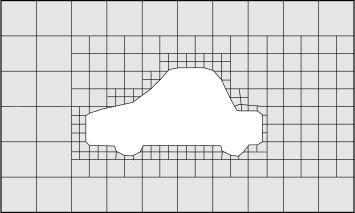
\includegraphics{fig-5-15}
 \caption{\OFtool{snappyHexMesh}における表面のスナップ}
 \label{fig:5.15}
\end{figure}


\subsection{メッシュレイヤ}
\label{ssec:5.4.7}
\index{snappyHexMesh@\OFtool{snappyHexMesh}!ユーティリティ!メッシュレイヤ}%
境界面に沿った不規則なセルを作りもしますが,
スナップによるメッシュの生成は目的に合致するでしょう.
メッシュをかける過程にはさらにオプションがあり,
\autoref{fig:5.16}の暗く影のついた部分が示すように,
境界面に沿って並べられた六面体のセルのレイヤを追加します.


\begin{figure}[ht]
 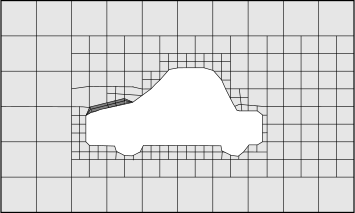
\includegraphics{fig-5-16}
 \caption{レイヤの挿入}
 \label{fig:5.16}
\end{figure}


メッシュのレイヤの追加は,
以下の手順のように既存のメッシュを境界から縮小させ,
レイヤを挿入することで行われます.
\begin{enumerate}
 \item 表面に対して法線方向の厚み分だけメッシュを投影させる.
 \item\label{enm:5.4.7-2}
      最後に移動した境界面の頂点をもとに内部メッシュの緩和を計算する
 \item 有効性を確認し,満足されていない場合は投影された厚みを減らし,
       \ref{enm:5.4.7-2}からやり直す.
       いかなる厚みでも有効性が満足できない場合はレイヤを挿入しない.
 \item 有効性が確認できたらレイヤメッシュを挿入する.
 \item メッシュを再度チェックし,不良箇所が見られる場合は
       レイヤを除去し\ref{enm:5.4.7-2}に戻る.
\end{enumerate}

レイヤの追加の手順は\OFdictionary{snappyHexMeshDict}の
\OFsubdictionary{addLayersControls}サブディクショナリの設定によって行われます.
入力されるものは\autoref{tbl:5.10}に示すとおりです.


\begin{table}[ht]
 %#! platex UserGuideJa
\begin{tabularx}{\textwidth}{lXl}
 キーワード & 意味 & 例 \\
 \hline
\index{layers@\OFkeyword{layers}!キーワード}%
\index{キーワード!layers@\OFkeyword{layers}}%
 \OFkeyword{layers} &
     レイヤのディクショナリ &
          \\
\index{relativeSizes@\OFkeyword{relativeSizes}!キーワード}%
\index{キーワード!relativeSizes@\OFkeyword{relativeSizes}}%
 \OFkeyword{relativeSizes} &
     レイヤ厚さを,レイヤ外部の歪んでいないセルの大きさに対する相対値とするか,
     または絶対値とするか &
         \OFkeyword{true}/\OFkeyword{false} \\
\index{expansionRatio@\OFkeyword{expansionRatio}!キーワード}%
\index{キーワード!expansionRatio@\OFkeyword{expansionRatio}}%
 \OFkeyword{expansionRatio} &
     レイヤメッシュの拡大比率 &
         \OFkeyword{1.0} \\
\index{finalLayerRatio@\OFkeyword{finalLayerRatio}!キーワード}%
\index{キーワード!finalLayerRatio@\OFkeyword{finalLayerRatio}}%
 \OFkeyword{finalLayerRatio} &
     壁から最も遠い層の厚さ.
     \OFkeyword{relativeSizes}エントリにより相対値か絶対値かが決まる &
         \OFkeyword{0.3} \\
\index{minThickness@\OFkeyword{minThickness}!キーワード}%
\index{キーワード!minThickness@\OFkeyword{minThickness}}%
 \OFkeyword{minThickness} &
     セルのレイヤの最小の厚さ.
     相対値または絶対値(同上) &
         \OFkeyword{0.25} \\
\index{nGrow@\OFkeyword{nGrow}!キーワード}%
\index{キーワード!nGrow@\OFkeyword{nGrow}}%
 \OFkeyword{nGrow} &
     点がなければ生成されない面に結合されたレイヤの数.輪郭に近いレイヤ追加の収束に役立つ. &
         \OFkeyword{1} \\
\index{featureAngle@\OFkeyword{featureAngle}!キーワード}%
\index{キーワード!featureAngle@\OFkeyword{featureAngle}}%
 \OFkeyword{featureAngle} &
     この角度以上では表面は押し出されない &
         \OFkeyword{60} \\
\index{nRelaxIter@\OFkeyword{nRelaxIter}!キーワード}%
\index{キーワード!nRelaxIter@\OFkeyword{nRelaxIter}}%
 \OFkeyword{nRelaxIter} &
     緩和反復のスナップ最大数 &
         \OFkeyword{5} \\
\index{nSmoothSurfaceNormals@\OFkeyword{nSmoothSurfaceNormals}!キーワード}%
\index{キーワード!nSmoothSurfaceNormals@\OFkeyword{nSmoothSurfaceNormals}}%
 \OFkeyword{nSmoothSurfaceNormals} &
     表面法線のスムージング反復数 &
         \OFkeyword{1} \\
\index{nSmoothNormals@\OFkeyword{nSmoothNormals}!キーワード}%
\index{キーワード!nSmoothNormals@\OFkeyword{nSmoothNormals}}%
 \OFkeyword{nSmoothNormals} &
     内部メッシュの運動方向のスムージング反復数 &
         \OFkeyword{3} \\
\index{nSmoothThickness@\OFkeyword{nSmoothThickness}!キーワード}%
\index{キーワード!nSmoothThickness@\OFkeyword{nSmoothThickness}}%
 \OFkeyword{nSmoothThickness} &
     表面パッチ上の滑らかなレイヤの厚さ &
         \OFkeyword{10} \\
\index{maxFaceThicknessRatio@\OFkeyword{maxFaceThicknessRatio}!キーワード}%
\index{キーワード!maxFaceThicknessRatio@\OFkeyword{maxFaceThicknessRatio}}%
 \OFkeyword{maxFaceThicknessRatio} &
     極端にゆがんでいるセルでレイヤの生成を止める &
         \OFkeyword{0.5} \\
\index{maxThicknessToMedialRatio@\OFkeyword{maxThicknessToMedialRatio}!キーワード}%
\index{キーワード!maxThicknessToMedialRatio@\OFkeyword{maxThicknessToMedialRatio}}%
 \OFkeyword{maxThicknessToMedialRatio} &
     中間の距離と厚さの比が大きくなるとレイヤの生成を減少する &
         \OFkeyword{0.3} \\
\index{minMedianAxisAngle@\OFkeyword{minMedianAxisAngle}!キーワード}%
\index{キーワード!minMedianAxisAngle@\OFkeyword{minMedianAxisAngle}}%
 \OFkeyword{minMedianAxisAngle} &
     中間の軸点選択に使う角度 &
         \OFkeyword{130} \\
\index{nBufferCellsNoExtrude@\OFkeyword{nBufferCellsNoExtrude}!キーワード}%
\index{キーワード!nBufferCellsNoExtrude@\OFkeyword{nBufferCellsNoExtrude}}%
 \OFkeyword{nBufferCellsNoExtrude} &
     新しいレイヤの末端のためのバッファ領域を作成 &
         \OFkeyword{0} \\
\index{nLayerIter@\OFkeyword{nLayerIter}!キーワード}%
\index{キーワード!nLayerIter@\OFkeyword{nLayerIter}}%
 \OFkeyword{nLayerIter} &
     レイヤを追加する反復計算全体の最大反復数 &
         \OFkeyword{50} \\
\index{nRelaxedIter@\OFkeyword{nRelaxedIter}!キーワード}%
\index{キーワード!nRelaxedIter@\OFkeyword{nRelaxedIter}}%
 \OFkeyword{nRelaxedIter} &
     この反復回数を超えた後は,\OFkeyword{meshQuality}の
     \OFsubdictionary{relaxed}サブディクショナリにおける制御値が使われる &
         \OFkeyword{20} \\
 \hline
\end{tabularx}

 \caption{\OFpath{snappyHexMeshDict}の\OFsubdictionary{addLayersControls}サブディクショナリのキーワード}
 \label{tbl:5.10}
\end{table}


レイヤのサブディクショナリはレイヤが適用される各パッチと
必要な表面レイヤの数の入力を含んでいます.
パッチ名は,レイヤ追加が表面幾何形状ではなく
既存メッシュに関連付けられるので使われ,
したがって,表面領域ではなく,パッチに適用されます.
レイヤの入力例は以下のとおりです.
\begin{OFverbatim}[file]
 layers
  {
      sphere.stl_firstSolid
      {
          nSurfaceLayers 1;
      }
      maxY
      {
          nSurfaceLayers 1;
      }
  }
\end{OFverbatim}


\begin{table}[ht]
 %#! platex UserGuideJa
\begin{tabularx}{\textwidth}{lXl}
 キーワード & 意味 & 例 \\
 \hline
\index{maxNonOrtho@\OFkeyword{maxNonOrtho}!キーワード}%
\index{キーワード!maxNonOrtho@\OFkeyword{maxNonOrtho}}%
 \OFkeyword{maxNonOrtho} &
     非直交性上限角.\OFkeyword{180}は不可 &
         \OFkeyword{65} \\
\index{maxBoundarySkewness@\OFkeyword{maxBoundarySkewness}!キーワード}%
\index{キーワード!maxBoundarySkewness@\OFkeyword{maxBoundarySkewness}}%
 \OFkeyword{maxBoundarySkewness} &
     境界面ひずみ上限値.${} < 0$は不可 &
         \OFkeyword{20} \\
\index{maxInternalSkewness@\OFkeyword{maxInternalSkewness}!キーワード}%
\index{キーワード!maxInternalSkewness@\OFkeyword{maxInternalSkewness}}%
 \OFkeyword{maxInternalSkewness} &
     内部面ひずみ上限値.${} < 0$は不可 &
         \OFkeyword{4} \\
\index{maxConcave@\OFkeyword{maxConcave}!キーワード}%
\index{キーワード!maxConcave@\OFkeyword{maxConcave}}%
 \OFkeyword{maxConcave} &
     凹み上限角.\OFkeyword{180}は不可 &
         \OFkeyword{80} \\
\index{minFlatness@\OFkeyword{minFlatness}!キーワード}%
\index{キーワード!minFlatness@\OFkeyword{minFlatness}}%
 \OFkeyword{minFlatness} &
     実際の領域に対する最小の投影面積比率.\OFkeyword{-1}は不可 &
         \OFkeyword{0.5} \\
\index{minVol@\OFkeyword{minVol}!キーワード}%
\index{キーワード!minVol@\OFkeyword{minVol}}%
 \OFkeyword{minVol} &
     最小のピラミッドボリューム.大きな絶対値の負の数(例えば\OFkeyword{-1e30})は不可 &
         \OFkeyword{1e-13} \\
\index{minArea@\OFkeyword{minArea}!キーワード}%
\index{キーワード!minArea@\OFkeyword{minArea}}%
 \OFkeyword{minArea} &
     最小面領域.${} < 0$は不可 &
         \OFkeyword{} \\
\index{minTwist@\OFkeyword{minTwist}!キーワード}%
\index{キーワード!minTwist@\OFkeyword{minTwist}}%
 \OFkeyword{minTwist} &
     最小面ねじれ.${} < -1$は不可 &
         \OFkeyword{0.05} \\
\index{minDeterminant@\OFkeyword{minDeterminant}!キーワード}%
\index{キーワード!minDeterminant@\OFkeyword{minDeterminant}}%
 \OFkeyword{minDeterminant} &
     最小正常セルの行列式.$\mbox{\OFkeyword{1}} = \mbox{\OFkeyword{hex}}$,${} \le 0$は不法なセル &
         \OFkeyword{0.001} \\
\index{minFaceWeight@\OFkeyword{minFaceWeight}!キーワード}%
\index{キーワード!minFaceWeight@\OFkeyword{minFaceWeight}}%
 \OFkeyword{minFaceWeight} &
     $\mbox{\OFkeyword{0}} \rightarrow \mbox{\OFkeyword{0.5}}$ &
         \OFkeyword{0.05} \\
\index{minVolRatio@\OFkeyword{minVolRatio}!キーワード}%
\index{キーワード!minVolRatio@\OFkeyword{minVolRatio}}%
 \OFkeyword{minVolRatio} &
     $\mbox{\OFkeyword{0}} \rightarrow \mbox{\OFkeyword{1.0}}$ &
         \OFkeyword{0.01} \\
\index{minTriangleTwist@\OFkeyword{minTriangleTwist}!キーワード}%
\index{キーワード!minTriangleTwist@\OFkeyword{minTriangleTwist}}%
 \OFkeyword{minTriangleTwist} &
     Fluent計算可能性では${} > 0$ & \\
\index{nSmoothScale@\OFkeyword{nSmoothScale}!キーワード}%
\index{キーワード!nSmoothScale@\OFkeyword{nSmoothScale}}%
 \OFkeyword{nSmoothScale} &
     エラー分布反復数 &
         \OFkeyword{4} \\
\index{errorReduction@\OFkeyword{errorReduction}!キーワード}%
\index{キーワード!errorReduction@\OFkeyword{errorReduction}}%
 \OFkeyword{errorReduction} &
     エラー点の置換のための減少量 &
         \OFkeyword{} \\
 \hline
\end{tabularx}

 \caption{\OFdictionary{snappyHexMeshDict}の
 \OFsubdictionary{meshQualityControls}サブディクショナリのキーワード}
 \label{tbl:5.11}
\end{table}


\subsection{メッシュの品質制御}
\label{ssec:5.4.8}
メッシュの品質は\OFdictionary{snappyHexMeshDict}の
\OFsubdictionary{meshQualityControls}サブディクショナリへ入力することで
制御できます.入力は\autoref{tbl:5.11}に示します.



\section{メッシュの変換}
\label{sec:5.5}
ユーザは,他のパッケージを使用してメッシュを生成し,
OpenFOAMが用いる形式にそれらを変換できます.
\autoref{tbl:3.6}に示したような
様々なメッシュ変換ユーティリティが用意されています.

よく使われるメッシュ変換ユーティリティのいくつかを以下に挙げ,
使い方を紹介します.
\begin{description}
 \item[\OFtool{fluentMeshToFoam}]
\index{fluentMeshToFoam@\OFtool{fluentMeshToFoam}!ユーティリティ}%
\index{ユーティリティ!fluentMeshToFoam@\OFtool{fluentMeshToFoam}}%
            \OFemph{Fluent}の\texttt{.msh}メッシュファイルを読み込みます.
            2次元,3次元両方に使えます.
 \item[\OFtool{starToFoam}]
\index{starToFoam@\OFtool{starToFoam}!ユーティリティ}%
\index{ユーティリティ!starToFoam@\OFtool{starToFoam}}%
            \OFemph{STAR-CD}/\OFemph{PROSTAR}のメッシュファイルを読み込みます.
 \item[\OFtool{gambitToFoam}]
\index{gambitToFoam@\OFtool{gambitToFoam}!ユーティリティ}%
\index{ユーティリティ!gambitToFoam@\OFtool{gambitToFoam}}%
            \OFemph{GAMBIT}の\texttt{.neu}ニュートラルファイルを読み込みます.
 \item[\OFtool{ideasToFoam}]
\index{ideasToFoam@\OFtool{ideasToFoam}!ユーティリティ}%
\index{ユーティリティ!ideasToFoam@\OFtool{ideasToFoam}}%
            \OFemph{ANSYS}の\texttt{.ans}形式で書かれた
            \OFemph{I-DEAS}メッシュを読み込みます.
 \item[\OFtool{cfx4ToFoam}]
\index{cfx4ToFoam@\OFtool{cfx4ToFoam}!ユーティリティ}%
\index{ユーティリティ!cfx4ToFoam@\OFtool{cfx4ToFoam}}%
            \texttt{.geo}形式で書かれた\OFemph{CFX}メッシュを読み込みます.
\end{description}


\subsection{\OFtool{fluentMeshToFoam}}
\label{ssec:5.5.1}
Fluentは,\texttt{.msh}拡張子をもつ単一のファイルに,
メッシュ・データを書き出します.
ASCII書式でファイルを書かなければなりませんが,
それは,Fluentのデフォルトの選択ではありません.
2次元の幾何形状を含んでいる単一の流れの
Fluentメッシュを変換することは可能です.
OpenFOAMでは,2次元幾何形状は,現在のところ,
3次元でメッシュを定義することで扱われます.
そこでは,前面と背面は\OFkeyword{empty}境界パッチタイプと定義されます.
2次元のFluentメッシュを読みこむときに,
コンバータは,自動的に3次元目の方向にメッシュを拡張し,
\OFkeyword{frontAndBackPlanes}と名づけ,空のパッチを加えます.

また,以下の特徴が見られます.
\begin{itemize}
 \item OpenFOAMコンバータは,
       Fluentの境界条件の定義をできるだけ把握しようと試みるでしょう.
       しかしながら,OpenFOAMとFluentの境界条件の間に明確で,
       直接的な対応は全くないので,
       ユーザはケースを実行する前に境界条件をチェックするべきです.
 \item 2次元メッシュから軸対称なメッシュを生成することは
       現在サポートされていませんが,ご要望があれば実装されるでしょう.
 \item 複数の媒質からなるメッシュは受入れられません.
       もし複数の流体媒質が存在していると,
       それらは単一のOpenFOAMメッシュに変換されるでしょう.
       もし固体領域が検出されると,
       コンバータは,それを排除しようと試みるでしょう.
 \item Fluentはメッシュの内部にパッチを定義することを
       ユーザに許しています.つまり,面の両側にセルが存在する場合です.
       そのようなパッチはOpenFOAMでは許容されていないので,
       コンバータはそれらを排除しようと試みるでしょう.
 \item 現在,埋め込まれたインタフェースと細分化の
       ツリーに関するサポートは全くありません.
\end{itemize}
Fluent \texttt{.msh}ファイルの変換は,
必要なディレクトリとファイルを作成することによって
まず新しいOpenFOAMケースを作ることで始まります.
ケースディレクトリは\OFpath{system}のサブディレクトリに
\OFdictionary{controlDict}ファイルを含みます.
そしてコマンド・プロンプトにおいて,ユーザは以下を実行することになります.
\begin{OFverbatim}[terminal]
fluentMeshToFoam <meshFile>
\end{OFverbatim}
ここで \texttt{<meshFile>} は絶対パスか相対パスによる
\texttt{.msh}ファイルの名前です.


\subsection{\OFtool{starToFoam}}
\label{ssec:5.5.2}
このセクションはSTAR-CDコードで生成されたメッシュを,
OpenFOAMのメッシュのクラスが読むことができる書式に変換する方法を説明します.
メッシュはSTAR-CDとともに供給されるどのパッケージでも生成できます.
例えばPROSTAR,SAMM,ProAMおよびそれらの派生物です.
コンバータは,統合された任意のカップルマッチングを含む
どんなただ一つの流れのメッシュも受け入れ,
すべてのセルタイプがサポートされます.
コンバータがサポートしない特徴は以下のとおりです.
\begin{itemize}
 \item 複数の流れのメッシュの仕様
 \item バッフル,すなわち,領域内に挿入された厚さなしの壁
 \item 部分境界,カップルマッチのうちの
       覆われていない部分は境界面であると考えられます.
 \item スライドするインターフェース
\end{itemize}
複数の流れのメッシュに関しては,
メッシュ変換は,別々のメッシュとして
それぞれの個々の流れを書くことによって実現され,
OpenFOAMでそれらを組み立て直すことができます.

OpenFOAMは,\autoref{sec:5.1}で指定された
かなり厳しい妥当性評価基準に整合しているメッシュの入力だけを
受け入れるという方針を採ります.
無効なメッシュを用いて実行されることはなく,
それ自体が無効なメッシュは変換できません.
以下のセクションは,STAR-CDとともに供給された
メッシュ生成パッケージを用いてメッシュを生成する際に,
OpenFOAM形式に変換できることを保証するために
取らなければならない方法を説明します.
これからのセクションにおいて重複を避けるために,
STAR-CDとともに供給されるメッシュ生成ツールは,
STAR-CDという総称によって参照されることにします.

\subsubsection{変換における一般的なアドバイス}
\label{sssec:5.5.2.1}
ユーザは\OFtool{starToFoam}の変換を試みる前に,
STAR-CDのメッシュをチェックするツールを動かすべきです.
そして,変換の後に,
\index{checkMesh@\OFtool{checkMesh}!ユーティリティ}%
\index{ユーティリティ!checkMesh@\OFtool{checkMesh}}%
\OFtool{checkMesh}ユーティリティは
新たに変換されたメッシュで実行されるべきです.
あるいはまた,\OFtool{starToFoam}はユーザが問題のあるセルを
より近くで見ることができるようにするための
\textsf{PROSTAR}コマンドを含む警告を発行するかもしれません.
問題の多いセルとマッチは,OpenFOAMを用いてメッシュを使おうとする前に,
チェックされ修正されるべきです.
無効なメッシュはOpenFOAMで動きませんが,
それが正当性評価基準を課さない別の環境では
動くかもしれないということを覚えていてください.

コンバータにおいて許容度を合わせることで,
許容度のマッチングに関するいくつかの問題を克服できます.
しかしながら,有効性への限界があり,
デフォルトレベルからマッチング許容度を増加させることが
明らかに必要であるということは,
オリジナルのメッシュが正確でないことを示します.

\subsubsection{不要なデータの消去}
\label{sssec:5.5.2.2}
メッシュ生成が終了したら,流体セルが作成されて,
他のすべてのセルが取り除かれると仮定して,
あらゆる不要な頂点を取り除き,
セル境界と頂点番号を圧縮してください.
これは以下の\textsf{PROSTAR}コマンドで実行されます.
\begin{OFverbatim}[terminal]
CSET NEWS FLUID
CSET INVE
\end{OFverbatim}
\texttt{CSET}は空であるべきです.これがそうでないなら,
\texttt{CSET}でセルを調べて,モデルを調整してください.
もしセルを本当に必要としていないなら,
\textsf{PROSTAR}コマンドを使用することでそれらを取り除くことができます.
\begin{OFverbatim}[terminal]
CDEL CSET
\end{OFverbatim}
同様に,頂点も取り除かれる必要があるでしょう.
\begin{OFverbatim}[terminal]
CSET NEWS FLUID
VSET NEWS CSET
VSET INVE
\end{OFverbatim}
これらの必要とされていない頂点を取り除く前に,
必要とされていない境界面は,除かれる前に,集められなければなりません.
\begin{OFverbatim}[terminal]
CSET NEWS FLUID
VSET NEWS CSET
BSET NEWS VSET ALL
BSET INVE
\end{OFverbatim}
\texttt{BSET}が空でないなら,必要とされていない境界面は
以下のコマンドを使用して削除することができます.
\begin{OFverbatim}[terminal]
BDEL BSET
\end{OFverbatim}
このとき,モデルは定義された境界面と同様に,
流体セルとそれを支持する頂点だけを含むべきです.
すべての境界面はセルの頂点によって完全に支えられるべきです.
もしそうでないなら,すべてが正常になるまで幾何学形状を正常化し続けます.

\subsubsection{デフォルトの境界条件の削除}
\label{sssec:5.5.2.3}
デフォルトで,STAR-CDは明示的に境界領域に関連づけられていない
どんな境界面に対して壁境界を適用します.
残っている境界面は,割り当てられた境界タイプ0として
\OFkeyword{default}境界領域に集められます.
OpenFOAMは,人為ミスを誘発するので,
意図的に未定義の界面のための\OFkeyword{default}境界条件の
概念をもっていません.
例えば,すべての関連付けられていない面に
デフォルト条件を意図して与えたかどうかをチェックする手段は全くありません.

したがって,メッシュが首尾よく変換されるために,
各OpenFOAMメッシュに対するすべての境界を指定しなければなりません.
default境界は,以下で説明された手順を用いることで
実体をもつものに変えられる必要があります.
\begin{enumerate}
 \item \OFkeyword{Wire Surface}オプションで幾何学形状をプロットしてください.
 \item \OFkeyword{default}領域0と同じパラメータで
       余分な境界領域を定義してください.
       そして,すべての見えている面を,
       境界ツールでゾーンオプションを選択して,
       モデルのスクリーンに描かれている全体の周りに多角形を描くことによって,
       10といった新しい領域に加えてください.
       \textsf{PROSTAR}の以下のコマンドを発行することによって,
       これができます.
\begin{OFverbatim}[terminal]
RDEF 10 WALL
BZON 10 ALL
\end{OFverbatim}
 \item 私たちはセットからすべての以前に定義された境界タイプを
       外すことになるでしょう.境界領域に行ってください.
\begin{OFverbatim}[terminal]
BSET NEWS REGI 1
BSET NEWS REGI 2
... 3, 4, ...
\end{OFverbatim}
       境界セットに関連している頂点を集め,
       次に頂点に関連している境界面を集めてください.
       それらは元のセットのように$2$倍あるでしょう.
\begin{OFverbatim}[terminal]
BSET NEWS REGI 1
VSET NEWS BSET
BSET NEWS VSET ALL
BSET DELE REGI 1
REPL
\end{OFverbatim}
       これは境界領域1の上で定義された境界領域10の面を与えるはずです.
       \verb|BDEL BSET|と共にそれらを削除してください.
       すべての領域にこれらを繰り返してください.
\end{enumerate}

\subsubsection{モデルの再番号付け}
\label{sssec:5.5.2.4}
コマンドを使用することでモデルの番号を付け替えて,チェックしてください.
\begin{OFverbatim}[terminal]
CSET NEW FLUID
CCOM CSET
VSET NEWS CSET
VSET INVE (Should be empty!)
VSET INVE
VCOM VSET
BSET NEWS VSET ALL
BSET INVE (Should be empty also!)
BSET INVE
BCOM BSET
CHECK ALL
GEOM
\end{OFverbatim}
内部の\textsf{PROSTAR}の照合は,最後の二つのコマンドで実行されます.
コマンドはいくつかの予見できない誤りを明らかにするかもしれません.
また,\textsf{PROSTAR}は幾何学形状にではなく,
STAR-CDのために因子を適用するだけであるので,
スケール因子に注意してください.因子が1でないなら,
OpenFOAMの
\index{scalePoints@\OFtool{scalePoints}!ユーティリティ}%
\index{ユーティリティ!scalePoints@\OFtool{scalePoints}}%
\OFtool{scalePoints}ユーティリティを使用してください.

\subsubsection{メッシュデータの出力}
\label{sssec:5.5.2.5}
メッシュがいったん完成されたら,
モデルのすべての統合されたマッチをカップルタイプ1に置いてください.
他のすべてのタイプが,任意のマッチを示すのに使用されるでしょう.
\begin{OFverbatim}[terminal]
CPSET NEWS TYPE INTEGRAL
CPMOD CPSET 1
\end{OFverbatim}
そして,計算格子の構成要素をそれら自身のファイルに書かなければなりません.
これはコマンドを発行し,境界に対して\textsf{PROSTAR}を用いることで行われます.
\begin{OFverbatim}[terminal]
BWRITE
\end{OFverbatim}
デフォルトでは,これは\texttt{.23}ファイル(3.0の前のバージョン)か
\texttt{.bnd}ファイル(バージョン3.0以降)に書きます.
セルに対しては,以下のコマンド,
\begin{OFverbatim}[terminal]
CWRITE
\end{OFverbatim}
がセルを\texttt{.14}か\texttt{.cel}ファイルに出力します.
頂点に対しては,以下のコマンド,
\begin{OFverbatim}[terminal]
VWRITE
\end{OFverbatim}
が\texttt{.15}か\texttt{.vrt}ファイルに出力します.
現在の既定の設定では,ASCII書式でファイルを書き出します.
カップルが存在しているなら,
拡張子\texttt{.cpl}をもつ追加カップルファイルが
以下のコマンドをタイプすることによって書きだされる必要があります.
\begin{OFverbatim}[terminal]
CPWRITE
\end{OFverbatim}
三つのファイルに出力した後に,\textsf{PROSTAR}を終了するか,
ファイルを閉じてください.
パネルに目を通して,すべてのSTAR-CDのサブモデル,
材料,および流体の特性に注目してください.
材料の特性と数学的モデルは,OpenFOAMディクショナリファイルを作成し,
編集することで設定される必要があるでしょう.

\textsf{PROSTAR}ファイルを変換する手順は最初に,
必要なディレクトリを作成することで新しいOpenFOAMのケースを作ることです.
同じディレクトリの中に\textsf{PROSTAR}ファイルを格納しなければなりません.
そして,ユーザはファイル拡張子を変えなければなりません.
\texttt{.23}と\texttt{.14}と\texttt{.15} (STAR-CDバージョン3.0以前) か,
\texttt{.pcs}と\texttt{.cls}と\texttt{.vtx} (STAR-CDバージョン3.0以降) から,
それぞれ\texttt{.bnd},\texttt{.cel},および\texttt{.vrt}に変えます.

\subsubsection{\texttt{.vrt}ファイルの問題}
\label{sssec:5.5.2.6}
\texttt{.vrt}ファイルは,フリー・フォーマットというよりむしろ
指定された幅に関するデータ列で書かれています.
座標値が続く頂点番号を与えるデータの典型的な行は,
以下のとおりであるかもしれません.
\begin{OFverbatim}[file]
19422 -0.105988957 -0.413711881E-02 0.000000000E+00
\end{OFverbatim}
縦座標が科学表記法で書かれていて,
負であるなら,値の間には,スペースが全くないかもしれません.
例えば以下のような状況です.
\begin{OFverbatim}[file]
19423 -0.953953117E-01-0.338810333E-02 0.000000000E+00
\end{OFverbatim}
\OFtool{starToFoam}コンバータは,
縦座標の値を区切るためにスペースを区切り文字としてデータを読むので,
前の例を読むとき,問題になります.
したがって,OpenFOAMは必要なところで値の間にスペースを挿入するための
簡単なスクリプト,
\index{foamCorrectVrt@\OFtool{foamCorrectVrt}!スクリプト/エイリアス}%
\index{スクリプト/エイリアス!foamCorrectVrt@\OFtool{foamCorrectVrt}}%
\OFtool{foamCorrectVrt}を含んでいます.
すると,それが前の例を以下のように変換するでしょう.
\begin{OFverbatim}[file]
19423 -0.953953117E-01 -0.338810333E-02 0.000000000E+00
\end{OFverbatim}
したがって,必要ならば\OFtool{starToFoam}コンバータを動かす前に,
以下のようにタイプすることで\OFtool{foamCorrectVrt}スクリプトを実行するべきです.
\begin{OFverbatim}[terminal]
foamCorrectVrt <file>.vrt
\end{OFverbatim}

\subsubsection{OpenFOAMのフォーマットへのメッシュの変換}
\label{sssec:5.5.2.7}
ここで,OpenFOAMの実行に必要な境界,セル,
およびポイントファイルを作成するために,
変換ユーティリティ\OFtool{starToFoam}を実行できます.
\begin{OFverbatim}[terminal]
starToFoam <meshFilePrefix>
\end{OFverbatim}
\texttt{<meshFilePrefix>} は,メッシュファイルの絶対か相対パスを
含んでいる接頭語の名前です.
ユーティリティの実行後に,OpenFOAM境界タイプは
\OFkeyword{boundary}ファイルを手で編集することによって指定されるべきです.


\subsection{\OFtool{gambitToFoam}}
\label{ssec:5.5.3}
GAMBITは\texttt{.neu}拡張子をもつ単一のファイルに
メッシュ・データを書き出します.
GAMBITの\texttt{.neu}ファイルを変換する手順は,
最初に新しいOpenFOAMケースを作成し,
そしてユーザがコマンド・プロンプトで以下のコマンドを実行します.
\begin{OFverbatim}[terminal]
gambitToFoam <meshFile>
\end{OFverbatim}
ここで \texttt{<meshFile>} は絶対か相対パスによる\texttt{.neu}ファイルの名前です.

GAMBITファイル形式は例えば,壁,対称面,周期境界といったような
境界パッチの種類に関する情報を提供しません.
したがって,すべてのパッチがタイプパッチとして作成されます.
メッシュ変換の後に必要に応じてリセットしてください.


\subsection{\OFtool{ideasToFoam}}
\label{ssec:5.5.4}
OpenFOAMはI-DEASによって生成されたメッシュを変換できますが,
\texttt{.ans}ファイルとしてANSYS形式で書きだされます.
\texttt{.ans}ファイルを変換する手順は最初に新しいOpenFOAMケースを作成し,
そしてユーザがコマンド・プロンプトから以下のように実行します.
\begin{OFverbatim}[terminal]
ideasToFoam <meshFile>
\end{OFverbatim}
ここで \texttt{<meshFile>} は絶対か相対パスによる\texttt{.ans}ファイルの名前です.


\subsection{\OFtool{cfx4ToFoam}}
\label{ssec:5.5.5}
CFXは\texttt{.geo}拡張子をもつ単一のファイルにメッシュ・データを書き出します.
CFXのメッシュ形式は,ブロック構造です.
すなわち,メッシュは相互の関係と頂点の位置の情報をもつブロックの組として指定されます.
OpenFOAMはメッシュを変換して,できるだけよくCFX境界条件を得ようと試みるでしょう.
単一のOpenFOAMメッシュに変換される全ての領域とともに,
多孔質や固体領域などに関する情報を含むCFXの3次元の「パッチ」定義は無視されます.
CFXは「デフォルト」パッチの概念をサポートし,
そこでは,境界条件が定義されていない外部の面のそれぞれが壁として扱われます.
これらの面はコンバータで集められ,
OpenFOAMメッシュの\OFkeyword{defaultFaces}パッチに入れられ,
タイプ\OFkeyword{wall}が与えられます.
もちろん,それに続けてパッチタイプを変えることができます.

CFXでのOpenFOAMの2次元幾何形状は,一つのセルの厚さ [**] の
3次元メッシュとして作成されます.
もしユーザがCFXによって作成されたメッシュで2次元のケースを動かしたいなら,
前後の面に関する境界条件は\OFkeyword{empty}として設定されるべきです.
ユーザは,計算面の他のすべての面に関する境界条件が
正しく設定されていることを確かめるべきです.
現在,2次元のCFXメッシュから軸対称の幾何形状を作成するための機能はありません.

CFXの\texttt{.geo}ファイルを変換する手順は
最初に新しいOpenFOAMケースを作成し,
そしてユーザがコマンド・プロンプトから以下のように実行します.
\begin{OFverbatim}[terminal]
cfx4ToFoam <meshFile>
\end{OFverbatim}
ここで \texttt{<meshFile>} は絶対か相対パスによる\texttt{.geo}ファイルの名前です.



\section{異なるジオメトリ間のフィールドマッピング}
\label{sec:5.6}
\index{マッピング!フィールド}%
\index{フィールド!マッピング}%
\OFtool{mapFields}ユーティリティは,
別のジオメトリに対応するフィールドに与えられたジオメトリに関連する
一つ以上のフィールドをマップします.
フィールドが関連するジオメトリの間のどんな類似性も必要とされないほど
完全に一般化されています.
しかしながら,ジオメトリが一貫している場合は,
マッピングの過程を簡素化する特別なオプションを用いて\OFtool{mapFields}を実行できます.

\OFtool{mapFields}について述べるために,
いくつかの用語を定義する必要があります.
まず,データがソースからターゲットまでマップされるといいます.
ソースとターゲットフィールドの両方の幾何形状と境界タイプ,
あるいは条件がまったく同じであるなら,フィールドは一貫していると考えられます.
\OFtool{mapFields}がマップするフィールド・データは,
ターゲットとなるケースの
\index{controlDict@\OFdictionary{controlDict}!ディクショナリ}%
\index{ディクショナリ!controlDict@\OFdictionary{controlDict}}%
\OFdictionary{controlDict}の
\OFsubdictionary{startFrom/startTime}によって指定された
時間ディレクトリの中のフィールドです.
データは,ソースとなるケースの同等な時間ディレクトリから読み込まれて,
ターゲットとなるケースの同等な時間ディレクトリに写像されます.


\subsection{一貫したフィールドのマッピング}
\label{ssec:5.6.1}
一貫したフィールドのマッピングは,
以下の \texttt{-consistent}コマンドラインオプションを使用しながら,
\index{mapFields@\OFtool{mapFields}!ユーティリティ}%
\index{ユーティリティ!mapFields@\OFtool{mapFields}}%
\OFtool{mapFields}を(ターゲット)ケース上で実行することによって,
簡単に実行されます.
\begin{OFverbatim}[terminal]
mapFields <source dir> -consistent
\end{OFverbatim}

\subsection{一貫しないフィールドのマッピング}
\label{ssec:5.6.2}
フィールドが\autoref{fig:5.17}のように一貫していないとき,
\OFtool{mapFields}はターゲットとなるケースの
\OFpath{system}ディレクトリに\OFpath{mapFieldsDict}ディクショナリを必要とします.
以下の規則がマッピングに適用されます.
\begin{itemize}
 \item フィールド・データはどこでも,可能である限り,
       ソースからターゲットにマップされます.
       すなわち,私たちの例では,
       代替されないままで残っている網掛け領域を除いて,
       ターゲットとなる幾何形状に含まれるすべてのフィールド・データが
       ソースからマップされます.
 \item 別の方法で\OFpath{mapFieldsDict}ディクショナリで指定されない限り,
       パッチフィールド・データは代替されないままです.
\end{itemize}
\OFpath{mapFieldsDict}ディクショナリは,
パッチデータに関するマッピングを指定する二つのリストを含んでいます.
最初のリストは,\autoref{fig:5.17}のように幾何形状が一致するソースと
ターゲットとなるパッチの組の間のデータのマッピングを指定する
\index{patchMap@\OFkeyword{patchMap}!キーワード}%
\index{キーワード!patchMap@\OFkeyword{patchMap}}%
\OFkeyword{patchMap}です.
リストは,ソースとターゲットとなるパッチの名前のそれぞれの組を含んでいます.
2番目のリストは,ターゲットとなるパッチの名前を含む
\OFkeyword{cuttingPatches}です.そのターゲットのパッチの値は,
ターゲットとなるパッチが切断するソースの内部のフィールドからマップされます.
私たちの例における左下のターゲットとなるパッチにように,
ターゲットとなるパッチがソースの内部の
フィールドの一部を切断するだけの状況では,
内部のフィールドに含まれるそれらの値はマップされ,
外部にある値は変わりません.
\OFpath{mapFieldsDict}ディクショナリの例は以下に示します.


\begin{figure}[ht]
 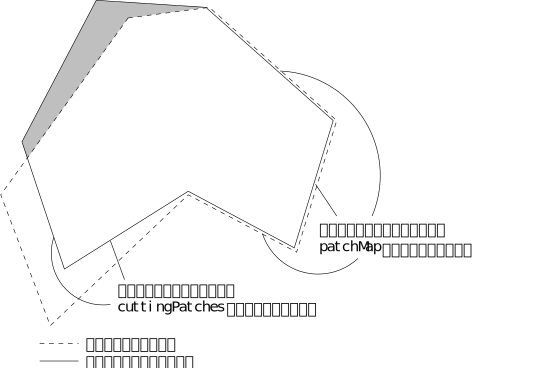
\includegraphics{fig-5-17}
 \caption{一貫しないフィールドをマップする}
 \label{fig:5.17}
\end{figure}

\begin{OFverbatim}[file, linenum=17]

patchMap        ( lid movingWall );

cuttingPatches  ( fixedWalls );


// ************************************************************************* //
\end{OFverbatim}

\begin{OFverbatim}[terminal]
mapFields <source dir>
\end{OFverbatim}


\subsection{並列なケースのマッピング}
\label{ssec:5.6.3}
\OFtool{mapFields}を実行するとき,
並列計算のためにソースとターゲットとなるケースの
どちらかもしくは両方を分解するなら,追加オプションが必要になります.
\begin{description}
 \item[\texttt{-parallelSource}] ソースケースが並列計算のために分解される場合
 \item[\texttt{-parallelTarget}] ターゲットケースが並列計算のために分解される場合
\end{description}

../../../UserGuideJa/chapter6.tex
%#! uplatex UserGuideJa
\chapter{モデルと物性値}
\label{chap:7}
OpenFOAMには,各々が特定の問題に特化して設計されたソルバが,
幅広い範囲にわたって用意されています.
ユーザは,特定のケースに対してモデリングを行う際に
最初にソルバの選択ができるように,
その方程式とアルゴリズムは一つ一つが異なったものとなっています.
ソルバの選択には,通常,\autoref{sec:3.5}にある各ソルバの説明に目を通して,
そのケースに対して適切なソルバを見つけてください.
各々のケースを定義するためには,
最終的にはパラメータと物理的特性が必要となりますが,
いくつかのモデリングのオプションはケースの
\index{constant@\OFpath{constant}!ディレクトリ}%
\index{ディレクトリ!constant@\OFpath{constant}}%
\OFpath{constant}ディレクトリの中のディクショナリに
登録されている中から実行時に指定することができます.
本章では,一般的なモデルと,実行時に指定すべき
関連プロパティについて詳しく説明します.



\section{熱物理モデル}
\label{sec:7.1}
熱物性モデルは,エネルギ,熱および物理的な特性が関与しています.
\index{thermophysical@\OFemph{thermophysical}!ライブラリ}%
\index{ライブラリ!thermophysical@\OFemph{thermophysical}}%
\OFemph{thermophysical}モデルライブラリを使用するあらゆるソルバは
\index{thermophysicalProperties@\OFdictionary{thermophysicalProperties}!ディクショナリ}%
\index{ディクショナリ!thermophysicalProperties@\OFdictionary{thermophysicalProperties}}%
\OFdictionary{thermophysicalProperties}ディクショナリを読み込みます.
OpenFOAMの熱物性モデルは圧力・温度 ($p$--$T$) システムとして構築され,
その他の物理量はそこから計算されます.
シミュレーションの中で使用する熱物性モデリングのパッケージを指定するために,
\index{thermoType@\OFkeyword{thermoType}!キーワード}%
\index{キーワード!thermoType@\OFkeyword{thermoType}}%
\OFkeyword{thermoType}と呼ばれる必須のディクショナリエントリがあります.
OpenFOAMには,C++テンプレートを用いたコンパイル済みの
モデリングの組み合わせが多く含まれています.
このコーディング方針では,状態方程式から始まり,
前のレイヤから物性を導き出す熱物理モデリングのレイヤを加えていくことにより,
熱物理モデリングのパッケージを組み立てます.
\OFkeyword{thermoType}内のキーワードエントリは,
それら複数のモデリングのレイヤと,それらを組み合わせる基礎をなす枠組みを表しています.
以下は\OFkeyword{thermoType}のエントリの一例です.
\begin{OFverbatim}[file]
thermoType
{
    type            hePsiThermo;
    mixture         pureMixture;
    transport       const;
    thermo          hConst;
    equationOfState perfectGas;
    specie          specie;
    energy          sensibleEnthalpy;
}
\end{OFverbatim}

このキーワード・エントリは,
例えば輸送 (\OFkeyword{transport}) を定数(粘性と熱拡散を定数)として,
理想気体の状態方程式 (%
\index{equationOfState@\OFkeyword{equationOfState}!キーワード}%
\index{キーワード!equationOfState@\OFkeyword{equationOfState}}%
\OFkeyword{equationOfState}) を使うといった,
熱物理モデルの選択を示しています.
それに加えて
\index{energy@\OFkeyword{energy}!キーワード}%
\index{キーワード!energy@\OFkeyword{energy}}%
\OFkeyword{energy}というキーワード・エントリがあり,
解析におけるエネルギの扱い方を指定することができます.
以下の項では,\OFkeyword{thermoType}パッケージにおける
エントリと選択肢について説明します.


\subsection{熱物理モデルと混合気モデル}
\label{ssec:7.1.1@3.0.1}
熱物理モデリングを使用しているソルバは,
それぞれ特定の熱物理モデルクラスのオブジェクトを使用します.
モデルクラスを以下にまとめます.
\begin{description}
 \item[\OFclass{psiThermo}]
            圧縮率$\psi = (RT)^{-1}$に基づく,組成不変の熱物理モデルです.
            ここで$R$はガス定数,$T$は温度です.
            \OFclass{psiThermo}を使用するソルバには,
            \OFpath{compressible}ファミリのソルバ (\OFtool{sonicFoam},
            \OFtool{rhoSimpleFoam}%
\footnote{訳注:原文では\OFtool{simpleFoam}となっているが,おそらく誤記.}%
            など,\OFtool{rhoPorousSimpleFoam}は除く),
            \OFtool{uncoupledKinematicParcelFoam},\OFtool{coldEngineFoam}があります.
 \item[\OFclass{rhoThermo}]
            密度$\rho$に基づく,組成不変の熱物理モデルです.
            \OFclass{rhoThermo}を使用するソルバには,
            \OFpath{heatTransfer}ファミリのソルバ (\OFtool{buoyantSimpleFoam},
            CHTソルバなど,Boussinesqソルバは除く),
            \OFtool{rhoPorousSimpleFoam},\OFtool{twoPhaseEulerFoam},
            および\OFtool{thermoFoam}があります.
 \item[\OFclass{psiReactionThermo}]
            $\psi$に基づく,化学反応を伴う混合気の熱物理モデルです.
            \OFclass{psiReactionThermo}を使用するソルバには,
            \OFpath{combustion}ソルバの多く,例えば\OFtool{sprayFoam},
            \OFtool{chemFoam},\OFtool{fireFoam},\OFtool{reactingFoam},
            そして\OFpath{lagrangian}ソルバのいくつか,例えば\OFtool{coalChemistryFoam}や
            \OFtool{reactingParcelFilmFoam}があります.
 \item[\OFclass{psiuReactionThermo}]
            未燃ガスの圧縮率$\psi_{\mathrm{u}}$に基づく,燃焼の熱物理モデルです.
            \OFclass{psiuReactionThermo}を使用するソルバには,
            層流火炎速度と反応進行度変数
\OFrevision{regress variableの訳として適切?}%
            に基づいて燃焼をモデル化する\OFpath{combustion}ソルバ,
            例えば\OFtool{XiFoame},\OFtool{PDRFoam},および\OFtool{engineFoam}があります.
 \item[\OFclass{rhoReactionThermo}]
            $\rho$に基づく,化学反応を伴う混合気の熱物理モデルです.
            \OFclass{rhoReactionThermo}を使用するソルバは,
            \OFpath{combustion}ソルバのいくつか,例えば\OFtool{rhoReactingFoam}や
            \OFtool{rhoReactingBuoyantFoam},
            そして\OFpath{lagrangian}ソルバのいくつか,例えば\OFtool{reactingParcelFoam},
            \OFtool{simpleReactingParselFoam}
 \item[\OFclass{multiphaseMixtureThermo}]
            多層流の熱物理モデルです.
            \OFclass{multiphaseMixtureThermo}を使用するソルバには,
            圧縮性の\OFpath{multiphase}界面捕獲ソルバ,
            例えば\OFtool{compressibleInterFoam}や\OFtool{compressibleMultiphaseInterFoam}があります.
\end{description}

\OFkeyword{type}キーワードは,基礎となる熱物理モデルを指定します.
選択肢は以下のとおりです.
\begin{description}
 \item[\OFkeyword{hePsiThermo}]
            \OFclass{psiThermo}や\OFclass{psiReactionThermo}に基づくソルバで使用します.
 \item[\OFkeyword{heRhoThermo}]
            \OFclass{rhoThermo},\OFclass{rhoReactionThermo},
            および\OFclass{multiphaseMixtureThermo}に基づくソルバで使用します.
 \item[\OFkeyword{heheuPsiThermo}]
            \OFclass{psiuReactionThermo}に基づくソルバで使用します.
\end{description}

\OFkeyword{mixture}は混合気の組成を指定します.
化学反応を伴わない熱物理モデルに通常使われる選択肢は,
組成の固定された混合気を表す\OFkeyword{pureMixture}です.
\OFkeyword{pureMixture}が指定された場合,
\OFsubdictionary{mixture}というサブディクショナリの中で熱物理モデルの係数を指定します.

化学反応を伴う熱物理モデルで必要となる,組成が変化する混合気の場合に対しては,
\OFkeyword{reacting\-Mixture}という選択肢が使われます.
\OFkeyword{foamChemistryFile}キーワードで指定したファイル内に,
化学種と化学反応を列挙します.
それから\OFkeyword{reactingMixture}モデルに必要となる熱物理モデルの係数は,
それぞれの化学種の名前がつけられたサブディクショナリ (例えば\OFsubdictionary{O2}や\OFsubdictionary{N2})
の中で指定します.

層流火炎速度と反応進行度変数
\OFrevision{regress variableの訳として適切?}%
に基づいた燃焼に対しては,
\OFkeyword{fuel},\OFkeyword{oxidant},および\OFkeyword{burnt\-Prod\-ucts}といった混合気の
組み合わせが構成成分となります.
この燃焼モデルに使用できる混合気モデルは,
\OFkeyword{homogeneousMixture},\OFkeyword{inhomogeneousMixture}および
\OFkeyword{very\-In\-ho\-mo\-ge\-ne\-ous\-Mix\-ture}です.

組成の変化するその他のモデルには,
\OFkeyword{egrMixture},\OFkeyword{multiComponentMixture}および
\OFkeyword{sin\-gle\-Step\-Reacting\-Mixture}があります.


\subsection{輸送モデル}
\label{ssec:7.1.2@3.0.1}
輸送モデリングは,粘性係数%
\footnote{訳注:原文にはdynamic viscosityとあるが,文脈からして動粘性係数ではない.}%
$\mu$,熱伝導率$\kappa$,熱拡散率$\alpha$(内部エネルギとエンタルピの方程式に用いられる)の
評価に関係します.
現在の\OFclass{transport}モデルは,以下に説明するとおりです.
\begin{description}
 \item[\OFclass{const}]
            $\mu$とPrandtl数$\nPr = c_{\mathrm{p}}\mu/\kappa$が一定であると仮定します.
            それぞれ単純にキーワード
\index{mu@\OFkeyword{mu}!キーワード}%
\index{キーワード!mu@\OFkeyword{mu}}%
            \OFkeyword{mu}および
\index{Pr@\OFkeyword{Pr}!キーワード}%
\index{キーワード!Pr@\OFkeyword{Pr}}%
            \OFkeyword{Pr}によって指定します.
 \item[\OFclass{sutherland}]
            $\mu$を温度$T$の関数として計算します.
            これには,Sutherland係数$A_{\mathrm{S}}$とSutherland温度$T_{\mathrm{S}}$が用いられ,
            キーワード
\index{As@\OFkeyword{As}!キーワード}%
\index{キーワード!As@\OFkeyword{As}}%
            \OFkeyword{As}および
\index{Ts@\OFkeyword{Ts}!キーワード}%
\index{キーワード!Ts@\OFkeyword{Ts}}%
            \OFkeyword{Ts}によって指定します.
            $\mu$は,次のように計算されます.
\begin{align}
 \label{eq:7.2}
 \mu = \frac{A_{\mathrm{S}}\sqrt{T}}{1 + T_{\mathrm{S}}/T}
\end{align}
 \item[\OFclass{polynomial}]
            $\mu$と$\kappa$を温度$T$の関数として,任意次数$N$の多項式から計算します.
            例えば,
\begin{align}
 \label{eq:7.2@3.0.1}
 \mu = \sum^{N-1}_{i=0}a_{1}T^{i}
\end{align}
\end{description}


\subsection{熱力学モデル}
\label{ssec:7.1.3@3.0.1}
熱力学モデルは,比熱$c_{\mathrm{p}}$の評価に関わるものであり,
そこから他の物性値が導出されます.
現在の\OFclass{thermo}モデルは,以下に示すとおりです.
\begin{description}
 \item[\OFclass{hConst}]
            $c_{\mathrm{p}}$と融解熱$H_{\mathrm{f}}$を定数と仮定します.
            単純に
\index{Cp@\OFkeyword{Cp}!キーワード}%
\index{キーワード!Cp@\OFkeyword{Cp}}%
            \OFkeyword{Cp}および
\index{Hf@\OFkeyword{Hf}!キーワード}%
\index{キーワード!Hf@\OFkeyword{Hf}}%
            \OFkeyword{Hf}というキーワードで
            二つの値$c_{\mathrm{p}}$と$H_{\mathrm{f}}$を指定します.
 \item[\OFclass{eConst}]
            $c_{\mathrm{v}}$と融解熱$H_{\mathrm{f}}$を定数と仮定します.
            単純に
\index{Cv@\OFkeyword{Cv}!キーワード}%
\index{キーワード!Cv@\OFkeyword{Cv}}%
            \OFkeyword{Cv}および
\index{Hf@\OFkeyword{Hf}!キーワード}%
\index{キーワード!Hf@\OFkeyword{Hf}}%
            \OFkeyword{Hf}というキーワードで
            二つの値$c_{\mathrm{v}}$と$H_{\mathrm{f}}$を指定します.
 \item[\OFclass{janaf}]
            熱力学の\OFemph{JANAF}表から得られた一連の係数により,
            $c_{\mathrm{p}}$を温度の関数として計算します.
            順に並べた係数のリストを\autoref{tbl:7.3}に示します.
            関数は,温度の下限$T_{\mathrm{l}}$と上限$T_{\mathrm{h}}$の間で妥当性が確認されています.
            係数は二組示されています.
            最初の組は常温$T_{\mathrm{c}}$以上 (そして$T_{\mathrm{h}}$以下) の温度についてのものであり,
            二組目は$T_{\mathrm{c}}$以下 (そして$T_{\mathrm{l}}$以上) の範囲のものです.
            $c_{\mathrm{p}}$を温度の関数として表すと,
\begin{align}
 \label{eq:7.1}
 c_{\mathrm{p}} = R((((a_{4}T + a_{3})T + a_{2})T + a_{1})T + a_{0})
\end{align}
            これに加えて,高温と低温の両方に$a_{5}$,$a_{6}$という積分定数があります.
            これらは,それぞれ$h$と$s$を評価するために使われます.
 \item[\OFclass{hPolynomial}]
            $c_{\mathrm{p}}$を温度の関数として,任意次数$N$の多項式によって計算します.
\begin{align}
 \label{eq:7.4@3.0.1}
 c_{\mathrm{p}} = \sum^{N-1}_{i=0}a_{1}T^{i}
\end{align}
            次のケースにその使用例があります:\\
            \hfil\OFpath{\$FOAM\_TUTORIALS/lagrangian/porousExplicitSourceReactingParcelFoam/filter}
\end{description}


\begin{table}[ht]
 %#! platex UserGuideJa
\begin{tabular}{lll}
 説明 & 入力 & キーワード \\
 \hline
 \tblstrut
 下限温度 & $T_{\mathrm{l}} \unit{(K)}$ & \OFkeyword{Tlow} \\
 上限温度 & $T_{\mathrm{h}} \unit{(K)}$ & \OFkeyword{Thigh} \\
 常温 & $T_{\mathrm{c}} \unit{(K)}$ & \OFkeyword{Tcommon} \\
 高温度係数 & $a_{0}$\ldots $a_{4}$ & \OFkeyword{highCpCoeffs (a0 a1 a2 a3 a4...} \\
 高温度エンタルピ補正 & $a_{5}$ & \OFkeyword{a5...} \\
 高温度エントロピ補正 & $a_{6}$ & \OFkeyword{a6)} \\
 低温度係数 & $a_{0}$\ldots $a_{4}$ & \OFkeyword{lowCpCoeffs (a0 a1 a2 a3 a4...} \\
 低温度エンタルピ補正 & $a_{5}$ & \OFkeyword{a5...} \\
 低温度エントロピ補正 & $a_{6}$ & \OFkeyword{a6)} \\
 \hline
\end{tabular}

 \caption{JANAFの熱力学係数}
 \label{tbl:7.3}
\end{table}


\subsection{各成分の組成}
\label{ssec:7.1.4@3.0.1}
現在のところ,各成分の組成を指定する\OFkeyword{specie}モデルに対する選択肢は一つだけです.
それ自身が\OFkeyword{specie}という名前であり,以下のエントリを指定します.
\begin{description}
 \item[\OFkeyword{nMoles}]
            成分のモル数を指定します.
            このエントリは,反応物質の均質な混合気と
            反応進行度変数に基づいた燃焼モデリングにのみ使用されます.
            それ以外の場合には1を指定します.
 \item[\OFkeyword{molWeight}]
            化学種のモルあたりグラム数を指定します.
\end{description}


\subsection{状態方程式}
\label{ssec:7.1.5@3.0.1}
熱物理モデリングにおいては以下のような状態方程式が使用できます.
\begin{description}
 \item[\OFclass{rhoConst}] 密度一定:
\begin{align}
 \label{eq:7.5@3.0.1}
 \rho = \text{constant.}
\end{align}
 \item[\OFclass{perfectGas}] 完全気体:
\begin{align}
 \label{eq:7.6@3.0.1}
 \rho = \frac{1}{RT}p
\end{align}
 \item[\OFclass{incompressiblePerfectGas}] 非圧縮性の完全気体:
\begin{align}
 \label{eq:7.7@3.0.1}
 \rho = \frac{1}{RT}p_{\mathrm{ref}}
\end{align}
            ここで$p_{\mathrm{ref}}$は参照圧力です.
 \item[\OFclass{perfectFluid}] 完全流体:
\begin{align}
 \label{eq:7.8@3.0.1}
 \rho = \frac{1}{RT}p + \rho_{0}
\end{align}
            ここで$\rho_{0}$は$T = 0$のときの密度です..
 \item[\OFclass{linear}] 線形の状態方程式:
\begin{align}
 \label{eq:7.9@3.0.1}
 \rho = \psi p + \rho_{0}
\end{align}
            ここで$\psi$は圧縮率です ($(RT)^{-1}$とはかぎりません).
 \item[\OFclass{adiabaticPerfectFluid}] 断熱の完全流体:
\begin{align}
 \label{eq:7.10@3.0.1}
 \rho = \rho_{0}\left(\frac{p + B}{p_{0} + B}\right)^{1/\gamma}
\end{align}
            ここで$\rho_{0}$,$p_{0}$はそれぞれ参照密度,圧力であり,
            $B$はモデル定数です.
 \item[\OFclass{PengRobinsonGas}] Peng Robinsonの状態方程式:
\begin{align}
 \label{eq:7.11@3.0.1}
 \rho = \frac{1}{zRT}p
\end{align}
            ここで複雑な関数$z = z(p,\ T)$は,
            \OFpath{\$FOAM\_SRC/thermophysicalModels/specie/equation\-Of\-State/}
            ディレクトリにある\OFpath{PengRobinsonI.H}ソースファイルで参照できます.
 \item[\OFclass{icoPolynomial}] 非圧縮性の多項式による状態方程式:
\begin{align}
 \label{eq:7.12@3.0.1}
 \rho = \sum^{N-1}_{i=1}a_{i}T^{i}
\end{align}
            ここで$a_{i}$は任意次数$N$の多項式に対する係数です.
\end{description}


\subsection{エネルギ変数の選択}
\label{ssec:7.1.6@3.0.1}
ユーザは,解析に使用するエネルギの形態を内部エネルギ$e$,エンタルピ$h$のいずれとするか,
そして生成熱$\Delta h_{\mathrm{f}}$を含めるかどうかを指定する必要があります.
この選択は\OFkeyword{energy}キーワードで指定します.

生成熱を含める場合は\emph{絶対}エネルギを使いますが,
そうでない場合は\emph{顕在}エネルギを使います.
例えば,絶対エンタルピ$h$と顕在エンタルピ$h_{\mathrm{s}}$の関係は以下のようになります.
\begin{align}
 \label{eq:7.1@2.2.0}
 h = h_{\mathrm{s}} + \sum_{i}c_{i}\Delta h_{\mathrm{f}}^{i}
\end{align}
ここで$c_{i}$と$h_{\mathrm{f}}^{i}$は,それぞれ化学種$i$のモル比と生成熱です.
ほとんどのケースにおいて,反応によるエネルギ変化を扱いやすいように,顕在エネルギを使います.
\index{energy@\OFkeyword{energy}!キーワード}%
\index{キーワード!energy@\OFkeyword{energy}}%
\OFkeyword{energy}に対するキーワード・エントリは,
例えば\OFkeyword{sensibleEnthalpy},\OFkeyword{sensibleInternalEnergy},
そして\OFkeyword{absoluteEnthalpy}などがあります.


\subsection{熱物性データ}
\label{ssec:7.1.1}
基本的な熱物性値は,各種類ごとに入力データに指定します.
データエントリには,\OFkeyword{O2},\OFkeyword{H2O},
\OFkeyword{mixture}といった物質名を示すキーワードに続けて,
以下のような係数のサブディクショナリを入力する必要があります.
\begin{description}
 \item[\OFkeyword{specie}]
\index{specie@\OFkeyword{specie}!キーワード}%
\index{キーワード!specie@\OFkeyword{specie}}%
            その物質のモル数
\index{nMoles@\OFkeyword{nMoles}!キーワード}%
\index{キーワード!nMoles@\OFkeyword{nMoles}}%
            \OFkeyword{nMoles},
            およびモル質量%
\footnote{訳注:原文ではmolecular weightとなっているので直訳すれば「モル重量」だが,
            単位が$\unit*{g/mol}$とされているので「モル質量」とした.}%
\index{molWeight@\OFkeyword{molweight}!キーワード}%
\index{キーワード!molWeight@\OFkeyword{molweight}}%
            \OFkeyword{molWeight}を$\unit*{g/mol}$の単位で入力します.
\index{thermodynamics@\OFkeyword{thermodynamics}!キーワード}%
\index{キーワード!thermodynamics@\OFkeyword{thermodynamics}}%
 \item[\OFkeyword{thermodynamics}] 選択した熱物理モデル(後述)に対する係数を入力します.
\index{transport@\OFkeyword{transport}!キーワード}%
\index{キーワード!transport@\OFkeyword{transport}}%
 \item[\OFkeyword{transport}] 選択した輸送モデル(後述)に対する係数を入力します.
\end{description}

以下は,\OFclass{sutherland}輸送モデルと\OFclass{janaf}熱力学モデルを用いた
\OFkeyword{fuel}という名前の種についての入力例です.
\index{Tlow@\OFkeyword{Tlow}!キーワード}%
\index{キーワード!Tlow@\OFkeyword{Tlow}}%
\index{Thigh@\OFkeyword{Thigh}!キーワード}%
\index{キーワード!Thigh@\OFkeyword{Thigh}}%
\index{Tcommon@\OFkeyword{Tcommon}!キーワード}%
\index{キーワード!Tcommon@\OFkeyword{Tcommon}}%
\index{highCpCoeffs@\OFkeyword{highCpCoeffs}!キーワード}%
\index{キーワード!highCpCoeffs@\OFkeyword{highCpCoeffs}}%
\index{lowCpCoeffs@\OFkeyword{lowCpCoeffs}!キーワード}%
\index{キーワード!lowCpCoeffs@\OFkeyword{lowCpCoeffs}}%
\begin{OFverbatim}[file]
fuel
{
    specie
    {
        nMoles       1;
        molWeight    16.0428;
    }
    thermodynamics
    {
        Tlow         200;
        Thigh        6000;
        Tcommon      1000;
        highCpCoeffs (1.63543 0.0100844 -3.36924e-06 5.34973e-10
                      -3.15528e-14 -10005.6 9.9937);
        lowCpCoeffs  (5.14988 -0.013671 4.91801e-05 -4.84744e-08
                      1.66694e-11 -10246.6 -4.64132);
    }
    transport
    {
        As           1.67212e-06;
        Ts           170.672;
    }
}
\end{OFverbatim}
次に示すのは,\OFclass{const}輸送モデルと\OFclass{hConst}熱力学モデルを用いた
\OFkeyword{air}という名前の物質についての入力例です.
\begin{OFverbatim}[file]
air
{
    specie
    {
        nMoles          1;
        molWeight       28.96;
    }
    thermodynamics
    {
        Cp              1004.5;
        Hf              2.544e+06;
    }
    transport
    {
        mu              1.8e-05;
        Pr              0.7;
    }
}
\end{OFverbatim}



\section{乱流モデル}
\label{sec:7.2}
乱流のモデリングを含むあらゆるソルバは
\index{turbulenceProperties@\OFdictionary{turbulenceProperties}!ディクショナリ}%
\index{ディクショナリ!turbulenceProperties@\OFdictionary{turbulenceProperties}}%
\OFdictionary{turbulenceProperties}ディクショナリを読み込みます.
このファイルの中では,
\index{simulationType@\OFkeyword{simulationType}!キーワード}%
\index{キーワード!simulationType@\OFkeyword{simulationType}}%
\OFkeyword{simulationType}キーワードで
使用する乱流モデルとして次のいずれかを選択します.
\begin{description}
 \item[laminar]
\index{laminar@\OFkeyword{laminar}!キーワードエントリ}%
\index{キーワードエントリ!laminar@\OFkeyword{laminar}}%
            乱流モデルを使用しない
 \item[RAS]
\index{RAS@\OFkeyword{RAS}!キーワードエントリ}%
\index{キーワードエントリ!RAS@\OFkeyword{RAS}}%
            Reynolds平均応力 (RAS) モデル
 \item[LES]
\index{LES@\OFkeyword{LES}!キーワードエントリ}%
\index{キーワードエントリ!LES@\OFkeyword{LES}}%
            ラージ・エディ・シミュレーション (LES) モデル
\end{description}

バージョン3.0.0以前のOpenFOAMに対する注記:
キーワードの選択肢は上記のかわりに\OFkeyword{RASModel}および\OFkeyword{LESModel}です.

\OFkeyword{RAS}が選択されているとき,
RASモデリングの選択は,同じく\OFpath{constant}ディレクトリにある\OFrevision{原文が誤記?}%
\OFsubdictionary{RAS}サブディクショナリで設定します.
RAS乱流モデルは,\autoref{tbl:3.9}に示した利用可能なモデルの長いリストから,
\OFkeyword{RASModel}エントリで選択します.
同様に,\OFkeyword{LES}が選択された場合,
LESモデリングの詳細は\OFsubdictionary{LES}ディクショナリで記述し,
LES乱流モデルは\OFkeyword{LESModel}エントリで選択します.

バージョン3.0.0以前のOpenFOAMに対する注記:
RASモデリングは\OFdictionary{turbulenceProperties}内の\OFsubdictionary{RAS}サブディクショナリではなく
独立した\OFdictionary{RASProperties}ファイルに,
同様にLESモデリングも独立した\OFdictionary{LESProperties}ファイルにて指定されます.

\OFsubdictionary{RAS}サブディクショナリに必要なエントリは\autoref{tbl:7.4}に,
また\OFsubdictionary{LES}サブディクショナリについては\autoref{tbl:7.5}に示します.


\begin{table}[ht]
 %#! platex UserGuideJa
\begin{tabular}{ll}
\index{RASmodel@\OFkeyword{RASmodel}!キーワード}%
\index{キーワード!RASmodel@\OFkeyword{RASmodel}}%
 \OFkeyword{RASModel} & RASモデルの名前 \\
\index{turbulence@\OFkeyword{turbulence}!キーワード}%
\index{キーワード!turbulence@\OFkeyword{turbulence}}%
 \OFkeyword{turbulence} & 乱流モデルのon/offスイッチ \\
\index{<RASmodel>Coeffs@\OFkeyword{<RASmodel>Coeffs}!キーワード}%
\index{キーワード!<RASmodel>Coeffs@\OFkeyword{<RASmodel>Coeffs}}%
 \OFkeyword{<RASModel>Coeffs} & 各RASModelにおける係数 \\
\index{wallFunctionCoeffs@\OFkeyword{wallFunctionCoeffs}!キーワード}%
\index{キーワード!wallFunctionCoeffs@\OFkeyword{wallFunctionCoeffs}}%
 \OFkeyword{wallFunctionCoeffs} & 壁関数の係数
\end{tabular}

 \caption{\OFsubdictionary{RAS}サブディクショナリにおけるキーワードエントリ}
 \label{tbl:7.4}
\end{table}


\begin{table}[ht]
 %#! platex UserGuideJa
\begin{tabular}{ll}
\index{LESmodel@\OFkeyword{LESmodel}!キーワード}%
\index{キーワード!LESmodel@\OFkeyword{LESmodel}}%
 \OFkeyword{LESmodel} & LESモデルの名前 \\
\index{delta@\OFkeyword{delta}!キーワード}%
\index{キーワード!delta@\OFkeyword{delta}}%
 \OFkeyword{delta} & デルタモデルの名前 \\
\index{<LESmodel>Coeffs@\OFkeyword{<LESmodel>Coeffs}!キーワード}%
\index{キーワード!<LESmodel>Coeffs@\OFkeyword{<LESmodel>Coeffs}}%
 \OFkeyword{<LESmodel>Coeffs} & 各LESモデルにおける係数 \\
\index{<delta>Coeffs@\OFkeyword{<delta>Coeffs}!キーワード}%
\index{キーワード!<delta>Coeffs@\OFkeyword{<delta>Coeffs}}%
 \OFkeyword{<delta>Coeffs} & 各デルタモデルにおける係数 \\
\index{kappa@\OFkeyword{kappa}!キーワード}%
\index{キーワード!kappa@\OFkeyword{kappa}}%
 \OFkeyword{kappa} & フォン・カルマン定数 \\
\index{wallFunctionCoeffs@\OFkeyword{wallFunctionCoeffs}!キーワード}%
\index{キーワード!wallFunctionCoeffs@\OFkeyword{wallFunctionCoeffs}}%
 \OFkeyword{wallFunctionCoeffs} & 壁関数の係数
\end{tabular}

 \caption{\OFsubdictionary{LES}サブディクショナリにおけるキーワードエントリ}
 \label{tbl:7.5}
\end{table}


非圧縮性および圧縮性のRAS乱流モデル,等容変化および非等容変化LESモデル,
そしてデルタモデルは,\autoref{tbl:3.9}に示しています.
これらの使用例は\OFpath{\$FOAM\_TUTORIALS}以下に見つかります.


\subsection{モデル係数}
\label{ssec:7.2.1}
RASモデルの係数には,それぞれのソースコードの中でデフォルト値が与えられています.
もしこのデフォルト値を上書きしたければ,
モデル名に\OFkeyword{Coeffs}を加えたキーワード名
(たとえば\OFkeyword{kEpsilon}モデルなら\OFkeyword{kEpsilonCoeffs})
のサブディクショナリを,
\OFdictionary{RASProperties}ファイルに追加することで実現できます.
もし\OFdictionary{RASProperties}ファイルで\OFkeyword{printCoeffs}スイッチが
\OFkeyword{on}になっていれば,
計算開始時にモデルが作成されたときに,
該当する\OFkeyword{\ldots Coeffs}ディクショナリの例が標準出力に表示されます.
ユーザは,これを\OFdictionary{RASProperties}にコピーして,
必要に応じて数値を変更すればよいでしょう.


\subsection{壁関数}
\label{ssec:7.2.2}
OpenFOAMでは,個別のパッチの境界条件として適用する,
様々な壁関数が利用可能になっています.
これにより,異なる壁領域に異なる壁関数モデルを適用することが可能になります.
壁関数モデルの選択は,\OFpath{0/nut}ファイル内の乱流粘性係数$\nu_{\mathrm{t}}$によって指定します.
バージョン3.0.0以前のOpenFOAMに対する注記:
圧縮性RASにおける壁関数は\OFpath{0/mut}ファイルの$\mu_{\mathrm{t}}$,
非圧縮性LESにおいては\OFpath{0/nuSgs}ファイルの$\nu_{\mathrm{sgs}}$,
圧縮性LESにおいては\OFpath{0/muSgs}ファイルの$\mu_{\mathrm{sgs}}$
によって指定します.
たとえば,ある\OFpath{0/nut}ファイルは,
\begin{OFverbatim}[file, linenum=17]

dimensions      [0 2 -1 0 0 0 0];

internalField   uniform 0;

boundaryField
{
    movingWall
    {
        type            nutkWallFunction;
        value           uniform 0;
    }
    fixedWalls
    {
        type            nutkWallFunction;
        value           uniform 0;
    }
    frontAndBack
    {
        type            empty;
    }
}


// ************************************************************************* //
\end{OFverbatim}
本リリースでは様々な壁関数モデルが利用できます.
例えば,\OFkeyword{nut\-Wall\-Function},
\OFkeyword{nut\-Rough\-Wall\-Function},\hskip.3em
\OFkeyword{nut\-U\-Spalding\-Wall\-Function},\hskip.3em
\OFkeyword{nutk\-Wall\-Function},\hskip.3em
そして\OFkeyword{nutk\-Atm\-Wall\-Function}などです.
関連するディレクトリを探すことにより,すべての壁関数モデルのリストを得ることができます.
\begin{OFverbatim}[terminal]
find $FOAM_SRC/turbulenceModels -name wallFunctions
\end{OFverbatim}%$

それぞれの壁関数境界条件では,
\OFkeyword{E},\OFkeyword{kappa},そして\OFkeyword{Cmu}という
オプションのキーワードエントリで$E$,$\kappa$,そして$C_{\mu}$のデフォルト値を上書きできます.
\OFpath{nut}や\OFpath{mut}ファイルのいずれかのパッチで壁関数を選択したならば,
\OFpath{epsilon}フィールドの対応するパッチでは\OFkeyword{epsilonWallFunction}を,
乱流場\OFpath{k},\OFpath{q},\OFpath{R}の対応するパッチには
\OFkeyword{kqRwallFunction}を選択する必要があります.



\section{輸送・流動モデル}
\label{sec:7.3@3.0.1}
OpenFOAMにおいて,エネルギや熱を含まないソルバは,粘性係数$\nu$のモデルライブラリを含みます.
これらのモデルは通常,粘性係数をひずみ速度$\dot{\gamma}$に関連付けるものであり,
\OFdictionary{transportProperties}ディクショナリで指定します.
以下の項に使用できるモデルを記載します.


\subsection{ニュートン流体モデル}
\label{ssec:7.3.1@3.0.1}
ニュートン流体モデルでは$\nu$は一定とみなします.
粘性係数は\OFdictionary{transportProperties}の中で\OFclass{dimensionedScalar}として指定します.
例えば,
\begin{OFverbatim}[file]
transportModel Newtonian;

nu             nu [ 0 2 -1 0 0 0 0 ] 1.5e-05;
\end{OFverbatim}
動粘性係数の次元は$\mathsf{L}^{2}/\mathsf{T}$であることに注意.


\subsection{Bird--Carreauモデル}
\label{ssec:7.3.2@3.0.1}
Bird--Carreauモデルは以下のとおりです.
\begin{align}
 \label{eq:7.14@3.0.1}
 \nu = \nu_{\infty} + (\nu_{0} - \nu_{\infty})[1 + (k\dot{\gamma})^{a}]^{(n-1)/a}
\end{align}
ここで,係数のデフォルト値は2です.
\OFdictionary{transportProperties}において,このモデルを指定する例を以下に示します.
\begin{OFverbatim}[file]
transportModel BirdCarreau;
BirdCarreauCoeffs
{
    nu0             nu0   [ 0 2 -1 0 0 0 0 ] 1e-03;
    nuInf           nuInf [ 0 2 -1 0 0 0 0 ] 1e-05;
    k               k     [ 0 0  1 0 0 0 0 ] 1;
    n               n     [ 0 0  0 0 0 0 0 ] 0.5;
}
\end{OFverbatim}


\subsection{Crossべき乗則モデル}
\label{ssec:7.3.3@3.0.1}
Crossのべき乗則モデルは以下のとおりです.
\begin{align}
 \label{eq:7.15@3.0.1}
 \nu = \nu_{\infty} + \frac{\nu_{0} - \nu_{\infty}}{1 + (m\dot{\gamma})^{n}}
\end{align}
\OFdictionary{transportProperties}において,このモデルを指定する例を以下に示します.
\begin{OFverbatim}[file]
transportModel CrossPowerLaw;
CrossPowerLawCoeffs
{
    nu0             nu0   [ 0 2 -1 0 0 0 0 ] 1e-03;
    nuInf           nuInf [ 0 2 -1 0 0 0 0 ] 1e-05;
    m               m     [ 0 0  1 0 0 0 0 ] 1;
    n               n     [ 0 0  0 0 0 0 0 ] 0.5;
}
\end{OFverbatim}


\subsection{べき乗則モデル}
\label{ssec:7.3.4@3.0.1}
べき乗則モデルは,最小値と最大値,
それぞれ$\nu_{\mathrm{min}}$および$\nu_{\mathrm{max}}$により制限された
粘性係数の関数を提供します.
この関数は以下のとおりです.
\begin{align}
 \label{eq:7.16@3.0.1}
 \nu &= k\dot{\gamma}^{n-1} &
 \nu_{\mathrm{min}} &\le \nu \le \nu_{\mathrm{max}}
\end{align}
\OFdictionary{transportProperties}において,このモデルを指定する例を以下に示します.
\begin{OFverbatim}[file]
transportModel powerLaw;
powerLawCoeffs
{
    nuMax           nuMax [ 0 2 -1 0 0 0 0 ] 1e-03;
    nuMin           nuMin [ 0 2 -1 0 0 0 0 ] 1e-05;
    k               k     [ 0 2 -1 0 0 0 0 ] 1e-05;
    n               n     [ 0 0  0 0 0 0 0 ] 1;
}
\end{OFverbatim}


\subsection{Herschel--Bulkleyモデル}
\label{ssec:7.3.5@3.0.1}
Herschel--Bulkleyモデルは,Bingham塑性体の効果と
流体のべき乗則の振る舞いを組み合わせます.
低ひずみ速度に対しては,材料は粘性係数$\nu_{0}$の高粘性流体としてモデル化されます.
限界応力$\tau_{0}$に対応する,ある閾値を超えるひずみ速度では,
粘性係数はべき乗則で記述されます.
このモデルは以下のとおりです.
\begin{align}
 \label{eq:7.17@3.0.1}
 \nu = \min\left(\nu_{0},\ \tau_{0}/\dot{\gamma} + k\dot{\gamma}^{n-1}\right)
\end{align}
\OFdictionary{transportProperties}において,このモデルを指定する例を以下に示します.
\begin{OFverbatim}[file]
transportModel HerschelBulkley;
HerschelBulkleyCoeffs
{
    nu0             nu0  [ 0 2 -1 0 0 0 0 ] 1e-03;
    tau0            tau0 [ 0 2 -2 0 0 0 0 ] 1;
    k               k    [ 0 2 -1 0 0 0 0 ] 1e-05;
    n               n    [ 0 0  0 0 0 0 0 ] 1;
}
\end{OFverbatim}



\backmatter
\makeatletter
\def\@linkcolor{blue}%
\makeatother
\printindex

\end{document}
